\documentclass[10pt,b5paper,twoside]{article} 
\usepackage[latin1]{inputenc}
\usepackage[english]{babel}
\usepackage{amsmath}
\usepackage{amsfonts}
\usepackage{amssymb}
\usepackage{makeidx}
\usepackage{graphicx}
\usepackage{hyperref}
\usepackage[left=2cm,right=2cm,top=2cm,bottom=2cm]{geometry}
\usepackage{float}
\usepackage{multirow}
\usepackage{verbatim} %for å kommentere ut ting
\usepackage[nottoc,numbib]{tocbibind}
\usepackage{chngpage} % allows for temporary adjustment of side margins
\usepackage[parfill]{parskip} %for avsnitt
\DeclareMathSizes{10}{10}{9}{9}
\usepackage{listings}
    \lstset{
            language=Matlab,                                % choose the language of the code
    %       basicstyle=10pt,                                % the size of the fonts that are used for the code
            numbers=left,                                   % where to put the line-numbers
            numberstyle=\footnotesize,                      % the size of the fonts that are used for the line-numbers
            stepnumber=1,                                           % the step between two line-numbers. If it's 1 each line will be numbered
            numbersep=5pt,                                  % how far the line-numbers are from the code
    %       backgroundcolor=\color{white},          % choose the background color. You must add \usepackage{color}
            showspaces=false,                               % show spaces adding particular underscores
            showstringspaces=false,                         % underline spaces within strings
            showtabs=false,                                         % show tabs within strings adding particular underscores
    %       frame=single,                                           % adds a frame around the code
    %       tabsize=2,                                              % sets default tabsize to 2 spaces
    %       captionpos=b,                                           % sets the caption-position to bottom
            breaklines=true,                                        % sets automatic line breaking
            breakatwhitespace=false,                        % sets if automatic breaks should only happen at whitespace
            escapeinside={\%*}{*)}                          % if you want to add a comment within your code
    }

\raggedbottom

\usepackage{makeidx}
\makeindex
%symbolliste slutt

\author{Anders Dall'Osso Teigset}
\title{MEDIUM VOLTAGE LOAD BREAK SWITCH WITH AIR AS INTERRUPTING MEDIUM}
\date{December, 2013}


\begin{document}
    \begin{titlepage}
    \begin{center}
    \ \\
    \ \\
    \ \\
    \ \\
    \ \\
    \ \\
    Anders Dall'Osso Teigset \\
    \ \\
    \ \\
    \ \\
    \ \\{\large \bfseries
    MEDIUM VOLTAGE LOAD BREAK SWITCH WITH AIR AS INTERRUPTING MEDIUM\\
    }
    \ \\
    \ \\
    \ \\
    \ \\
    \ \\
    {\large
    Specialisation project\\
    }
    \ \\
    {December, 2013 \\}
    \ \\
    \ \\
    \ \\
    \ \\
    \ \\
    \ \\
    \ \\
    \ \\
    \ \\
    \ \\
    \ \\
    \ \\
    \ \\
    \ \\
    \ \\
    \ \\
    \ \\
    \ \\
    \ \\
    \ \\
    \ \\
    \ \\
    \ \\
    \ \\
   	{\large
   Norwegian University of Science and Technology\\
   Department of Electric Power Engineering\\
    }
   	\ \\
    \ \\
    \end{center}
    \end{titlepage}

%\maketitle
%SummaryNyttige pdf-filer/SF6conduct.pdf
\thispagestyle{empty}
\cleardoublepage
\section*{Acknowledgements}
\setcounter{page}{1}
\pagenumbering{roman}

\cleardoublepage
\section*{Summary}

\cleardoublepage
\setcounter{page}{1}
\pagenumbering{arabic}
\tableofcontents
\cleardoublepage

\section{Introduction}
%HUSK AT DU KAN BRUKE NOE AV LYSBUE SPENNIGNSDUSKUSJONEN TIL Å FORKLARE. SE NOTAT FRA NINA.
\cleardoublepage

\section{Theory}
\subsection{Typical switchgear design and interruption sequence} \label{sec:genDes}
Most of the information in section \ref{sec:genDes} is collected from \textit{"Current Interruption in Power Grids"} by Magne Runde \cite{bib:HVEbreak} \newline

\subsubsection{Switchgear design and operation} \label{sec:InterruptCurrent}
Switchgear can be divided into four main categories:
\begin{itemize}
\item Disconnector Switch
\item Load Break Switch
\item Circuit Breaker
\item Earthing Switch
\end{itemize}

This report will focus on the load break switch (LBS) design. An LBS is designed to be able to interrupt currents with a magnitude equal to or less than the rated maximum continuous current in a at the location of the switchgear in the system. An LBS should fulfil the following demands in order to meet the requirements of the application area:

\begin{itemize}
\item When closed:
	\begin{itemize}
		\item Act as a good conductor.
		\item Be capable of interrupting any load that may arise, without generating too high over-voltages. 
	\end{itemize}
\item When open:
	\begin{itemize}
		\item Act as a good insulator.
		\item Be able to close without welding the contacts together, even under short-circuit conditions.
	\end{itemize}
\end{itemize}

A typical opening sequence for a switch is as follows: First, a control signal enters the switch and activates the driving mechanisms. In most cases, this is a compressed spring or a hydraulic system. The contacts begin to open, and a gap forms between them. At the same time, an electrical arc ignites between the contacts, burning in the gap. The gap is filled with some kind of interrupting medium which is usually a gas. When an altering current crosses zero, this is referred to as the current zero (CZ). For an alternating current with a frequency of 50 Hz, CZ will occur 100 times per second. Direct current interruptions will not be considered in this report.

%bilde som viser driving mechanisms compressed spring contacts?

At the CZ, the arc will extinguish for at least a moment, because the current is zero, and a voltage will build up between the contacts. This voltage is called the recovery voltage, and is defined in equation \eqref{eq:U_rec}, where $u_{supply}$ is the voltage on the supply side and $u_{load}$ is the voltage on the load side of the open switch. Depending on the recovery voltage two possible scenarios can occur: a re-ignition or a successful quenching of the arc. This is primary dependent on the steepness and the amplitude of the recovery voltage. There are two different kinds of re-ignition: thermal and dielectric. Thermal re-ignition takes place right after CZ, up to a few microseconds, and is mainly dependent on the steepness of the recovery voltage. As the recovery voltage rises and if a thermal re-ignition is avoided, a dielectric re-ignition may occur. This kind of re-ignition is largely dependent on the amplitude of the recovery voltage, and will occur after a millisecond or more. This report will mainly address thermal re-ignition. The likelihood of a re-ignition  will not be de-terminated by the arcing voltage itself, but by how the interrupting medium used reacts on the arcing voltage. Important interruption properties of air are discussed in section \ref{sec:propOfInt} and \ref{sec:TherMalReConsid} in this report. Other design parameters like contact material, geometry, speed of the contact movement, and cooling mechanisms are also important to the interruption properties.

\begin{equation} \label{eq:U_rec}
u_\mathrm{{recovery}}=u_\mathrm{{supply}}-u_\mathrm{{load}}
\end{equation}  

The plasma state of an interrupting medium occurs when gas and metal vapour are heated to very high temperatures. At a certain point, the molecules in the gas decompose to ions, neutrons and free electrons. This mixture is called plasma, and it makes up for most of the components in which an electrical arc burns, except for arcs that burns in vacuum. Plasma is a good electrical conductor compared to a gas, which is an insulator. Vacuum arcs will not be featured in this report.

In most switchgear designs, it is common to have two contact sets: one called the main contact and another called the arcing contact. The main contact is the first contact to open and the last one to close. This is to ensure that an arc does not start to burn between the main contact. The arcing contact is the last contact to open, and the first one to close, and will ensure that the arc burns between the arcing contact and never between the main contact.

Since the main contact opens first and closes last, its main purpose in the switchgear is to act as a good conductor. Copper is a good conductor, and is commonly used to ensure that this aspect of the switch is met. Sometimes, the contact surface is plated with tin, gold, silver, or platinum in order to ensure an even lower contact resistance between the contacts. The main problem with electrical losses in the switch is heat generation, which may speed up metal creep and other ageing-related processes in the switch. Contacts made of aluminium are especially vulnerable to creeping.

The arcing contacts are designed to withstand the harsh conditions that occur when an arc burns between the contacts. The contact material has to meet strict requirements, and has to tolerate high temperatures and arc erosion, and avoid welding and other stresses that may apply when closing or opening an energized contact. Aluminium and copper are not fit for these tasks, since they will melt or erode from the stresses of an arc. It is common to use composites that consist of metals with good electrical conduction and heat-resistant oxides. For high current and voltage switches, it is possible to use a composite of silver or copper together with tungsten or tungsten carbide. These materials are highly heat-resistant, but they also have a high electrical resistance. The higher electrical resistance in the arcing contact compared to the main contact is, however, not a problem, since the current only flows through the arcing contact for a short period of time.

\subsubsection{The puffer principle} \label{sec:puffer}
This report is focused on LBSs, but most of the available literature is related to circuit breakers. Therefore, the following section presents the working principle of different gas blast mechanisms used in circuit breakers, although, circuit breakers are different from LBSs, the working principle of the gas blast mechanism is somewhat similar for both kinds of switchgear.

In order to quench the arc, several mechanisms and interrupting mediums can be applied. In a compact LBS based on SF$_6$, a puffer mechanism is often used. In order to obtain a successful interruption of an arc, the arc and interruption medium must be cooled down, and the charged particles and vaporised metal between the arcing contacts must be blown away. This is the main purpose of the puffer mechanism. The puffer mechanism is based on a piston, and it generates a gas flow in the switchgear in order to extinguish the arc. A typical design of this system consists of a fixed piston integrated inside the movable contact part. A gas reservoir trapped between the arcing contact and the piston is pushed out as the contact members move apart from each other. Figure \ref{fig:CircutBreakPuff1} displays a typical puffer design in a circuit breaker.

When SF$_6$ entered the industry in the 1960s, it was in the form of dual pressure breakers. The SF$_6$-based dual pressure breakers had one high pressure chamber, and one low pressure chamber. A valve from a high pressure chamber opened during opening operations, generating a high speed SF$_6$ blast, guided by a nozzle to hit the arc burning between the contacts in the low-pressure chamber. This design has two major disadvantages when using SF$_6$. The switch requires heating in order to maintain the pressure in the high-pressure chamber for preventing condensation of the SF$_6$ gas. It also uses a compressor for pumping the gas from the low-pressure chamber to the high-pressure chamber. This adds to the complexity of the switchgear, and may result in more maintenance. The double pressure design was replaced with the newer single pressure design. The single pressure design has only one pressure chamber with low pressure, except during interruptions, when the chamber itself becomes a high-pressure chamber.

The single pressure design uses a puffer or the self-blast mechanism to quench the arc, or in some cases a combination of both. The self-blast mechanism is a concept that uses the expansion of the gas for creating a pressure difference and a gas flow to cool the arc. Common for both puffer and self-blast mechanisms is that they do not use a compressor to generate the gas flow, but uses the energy stored in the switching mechanisms or generated from the blast itself to interrupt the arc. These mechanisms work the same way for both circuit breakers and load break switches, but will in a load break switch be smaller and less complex. This is because the currents and voltages are smaller, and therefore a lower pressure is needed to obtain a successful interruption.

\begin{figure} [H]
\centering
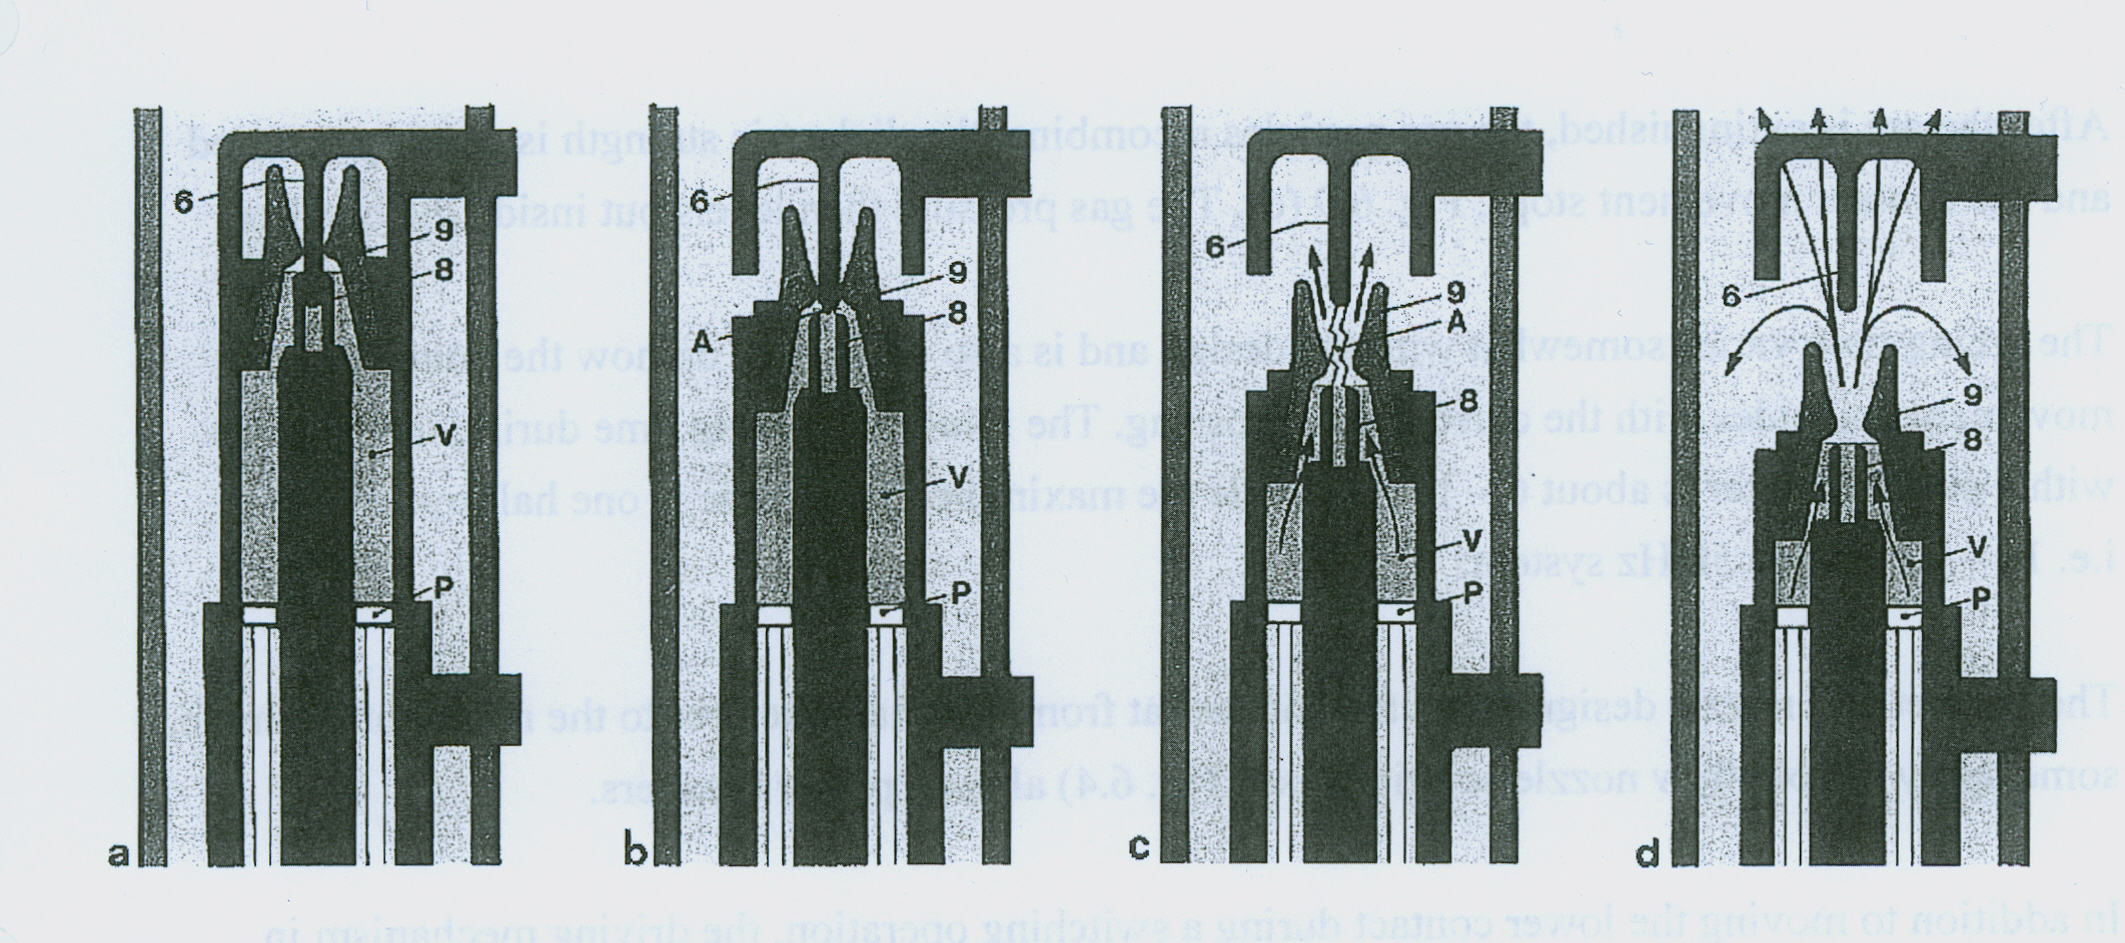
\includegraphics[scale=0.75]{Bilder/Theory/CircutBreakPuff1.png}
\caption{Interruption sequence in a circuit breaker using the puffer mechanism \cite{bib:HVEbreak}.} \label{fig:CircutBreakPuff1}
\end{figure}

Figure \ref{fig:CircutBreakPuff1} displays a typical interruption sequence of a circuit breaker based on the puffer design. When the breaker is closed, as illustrated in figure \ref{fig:CircutBreakPuff1}a, a gas volume \textit{(V)} is trapped between the piston \textit{(P)} and the arcing contact, \textit{(8)} and \textit{(6)}. During the period of time where the movable part of the arcing contact \textit{(8)} is pulled down, the volume decreases because of the placement of the fixed piston, and the pressure increases due to compression of the gas. Figure \ref{fig:CircutBreakPuff1}b illustrates the situation where the main contact is open and the current now only flows through the arcing contact.

The next stage of the interruption sequence is shown in figure \ref{fig:CircutBreakPuff1}c. The arcing contacts have now separated, and an arc \textit{(A)} has ignited between the contacts. The pressurised gas that previously was trapped between the piston and the arcing contact is now released. A nozzle \textit{(9)} that is fixed to the movable arcing contact guides the gas flow so that it will cool the arc down and blow away charge carriers between the contacts. If a sufficient gas flow is obtained, the arc will neither re-ignite after current zero, nor extinguish before current zero.

The gas flow is partly dependent on the cross-section of the arc, which again is dependent on the current amplitude. A large current resulting in a large arc may block the hole in the nozzle, preventing a gas flow. This is called current clogging, and may occur for certain nozzle designs at high current interruptions. In such an event, the pressure in the gas reservoir will increase further due to compression from mechanical moment of the arcing contact and thermal expansion in the gas, because of heating from the arc. When the current amplitude approaches zero, the arc's cross-section will decrease and the clogging effect will end. This will result in a powerful gas blast onto the arc, as indicated in figure \ref{fig:CircutBreakPuff1}d. For smaller current amplitudes, the arc cross-section is smaller, and a clogging effect does not occur to the same extent. This generates a less intense gas flow, preventing the current from being interrupted before its natural zero crossing.

The self-blast, or third generation breaker, was developed with the goal of reducing mechanical power of the operating system, making it cheaper and less complex. Figure \ref{fig:selfBlast} illustrates the working principle of a breaker using self-blast to interrupt an arc. The difference between self-blast and puffer mechanism is that the puffer mechanism increases the pressure by reducing the volume, while the self-blast design has a constant volume and relies on a rise in temperature to increase the gas pressure \cite{bib:CBAC}. The self-blast design uses the heat generated from an arc burning between the arcing contacts to interrupt the current. The gas expands as it is heated by the burning arc. This increase in pressure leads to a gas flow on the arc, which cools it down, leading to the arc being quenched.

\begin{figure} [H]
\centering
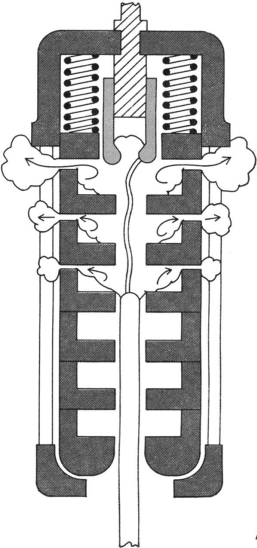
\includegraphics[scale=0.33]{Bilder/Theory/selfBlast.png}
\caption{Expulsion chamber in a circuit breaker using the self-blast mechanism \cite{bib:CBAC}.} \label{fig:selfBlast}
\end{figure}

There are some disadvantages of the self-blast principle when compared to the puffer mechanism. The self-blast has a lower dielectric strength, due to hot gas between the contacts after CZ. This gives a higher chance of re-ignition since hot gas has lower ionisation energy than cold gas. The design is also not well suited to break smaller currents. This is because the arc is less intense and therefore does not heat the gas sufficiently to create a strong enough blast. Therefore, it is common to combine self-blast and puffer mechanism in a hybrid design, so that it can handle both small and large currents. A compact LBS design using air as interrupting medium will probably rely on an active blowing mechanism like the puffer design. This is because an LBS faces smaller currents than a circuit breaker, making the self blast design unsuited.

A good circuit breaker design is difficult to develop, and the industry needs to optimise the product to meet the demands set by the market, such as size and pressure. This is due to high short-circuit currents in the range of 40 kA and large recovery voltages. Because of this, the industry has put a lot of effort into circuit breaker development. Nonetheless, when designing an LBS based on SF$_6$, it is common to take the working principle of a circuit breaker and scale it down to a suitable size for an LBS, and then test it. If it works, the LBS might be sold on the market without further alterations. Air is considered as a replacement for SF$_6$ as an interruption gas, due to the strong greenhouse gas potential of SF$_6$. When using air, this development technique has not been implemented successfully, since higher demands are set to the interrupting capabilities of the switchgear. This is because SF$_6$ is superior to air as an interrupting medium and the physical properties of the arc alters with the current. However, the same interruption techniques might be used, but with an increased focus on optimisation. In figure \ref{fig:selfBlastandPuffer}, the interrupter of a load break switch is shown. This is a down-scaled version of a circuit breaker, which has successfully been used to interrupt load current with SF$_6$ gas as interruption medium. 

\begin{figure} [H]
\centering
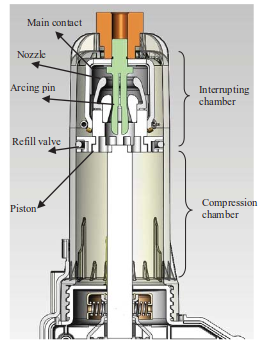
\includegraphics[scale=0.6]{Bilder/Theory/LBSselfblastandPuffer.png}
\caption{Schematic of a medium voltage gas puffer interrupter \cite{bib:CBAC}.} \label{fig:selfBlastandPuffer}
\end{figure}

As can been seen in figure \ref{fig:selfBlastandPuffer}, the load break switch features many of the same components as a circuit breaker, but the dimensions are scaled down. The interruption technique used is puffer based, and the operation sequence is the same as illustrated in figure \ref{fig:CircutBreakPuff1}. The article "Gas flow analysis in low energy arc puffer interrupters" \cite{bib:CBAC} presents an experiment where the the pressure in the pressure chamber of a LBS is measured during opening operation, and then is simulated, so that a comparison of the theoretical and measured pressures can be presented. In figure \ref{fig:airPressurePuffer}, the measured and simulated gas pressure from the paper are shown during a cold gas opening operation, which means that the switch was unloaded during the test. When certain loss factors have been included in the simulation, the simulation results correspond quite well with the measured pressures.


\begin{figure} [H]
\centering
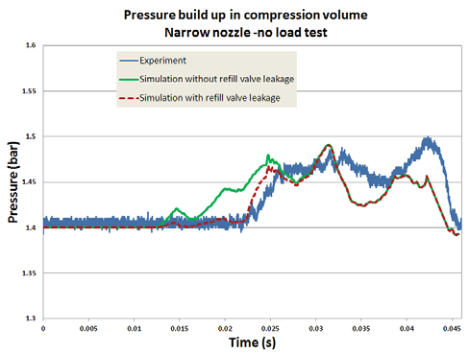
\includegraphics[scale=0.65]{Bilder/Theory/tankPressure.png}
\caption{Simulated pressure build up with different refill valve leakage settings compared to experimental results  \cite{bib:CBAC}.} \label{fig:airPressurePuffer}
\end{figure}

When introducing an arc to the system, the measured and simulated pressures change as shown in figure \ref{fig:airPressurePuffer2}. As seen in this figure, the pressure was not successfully simulated, and the difference between measured pressure and simulation results are substantial, and increases with a longer arcing time. This simulation technique has been used with success when simulating for circuit breakers. This gives reason to believe that the properties of the arc alters significantly when the current is reduced, as in a load break switch. Good simulation tools for air flows when arcs like this are present are still to be developed, which makes scaling a circuit breaker down to an LBS without the possibility to know how the arc interacts with the gas flow difficult, especially when using air as interruption medium, and not SF$_6$.



\begin{figure} [H]
\centering
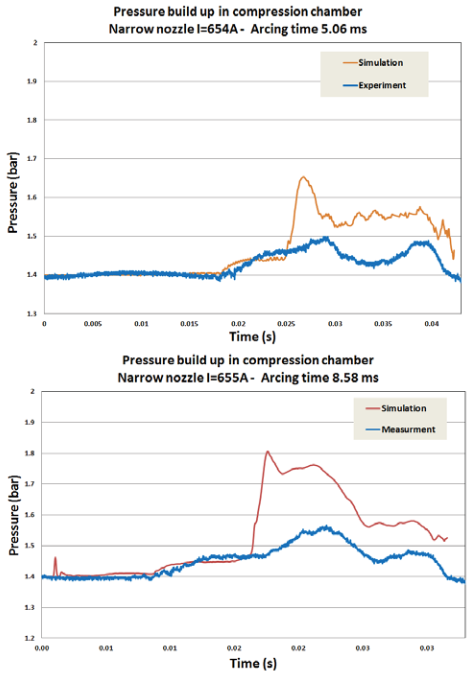
\includegraphics[scale=0.65]{Bilder/Theory/tankPressure2.png}
\caption{Pressure build up for load break tests with different arcing time   \cite{bib:CBAC}.} \label{fig:airPressurePuffer2}
\end{figure}

\subsection{Properties of the interrupting medium} \label{sec:propOfInt}
%As an interruption medium air is fairly good, and has been successfully used in the past to interrupt high currents at high voltages, some air-blast breakers are still in use. Dette hører kanskje inn i en innledning.
\subsubsection{Electrical conductivity in an arc} \label{sec:eleCondArc}
Gases have the ability to be good insulators as well as good conductors, mainly depending on the gas temperature. This is due to charged particles and electrons created by dissociation and ionisation of the molecules in the gas. Air is a mixture of several gases, but might be simplified to consist mostly of nitrogen (N$_2$). In figure \ref{fig:condAir}, the electrical conductivity of air as a function of temperature can be observed.

\begin{figure}[H]
\centering
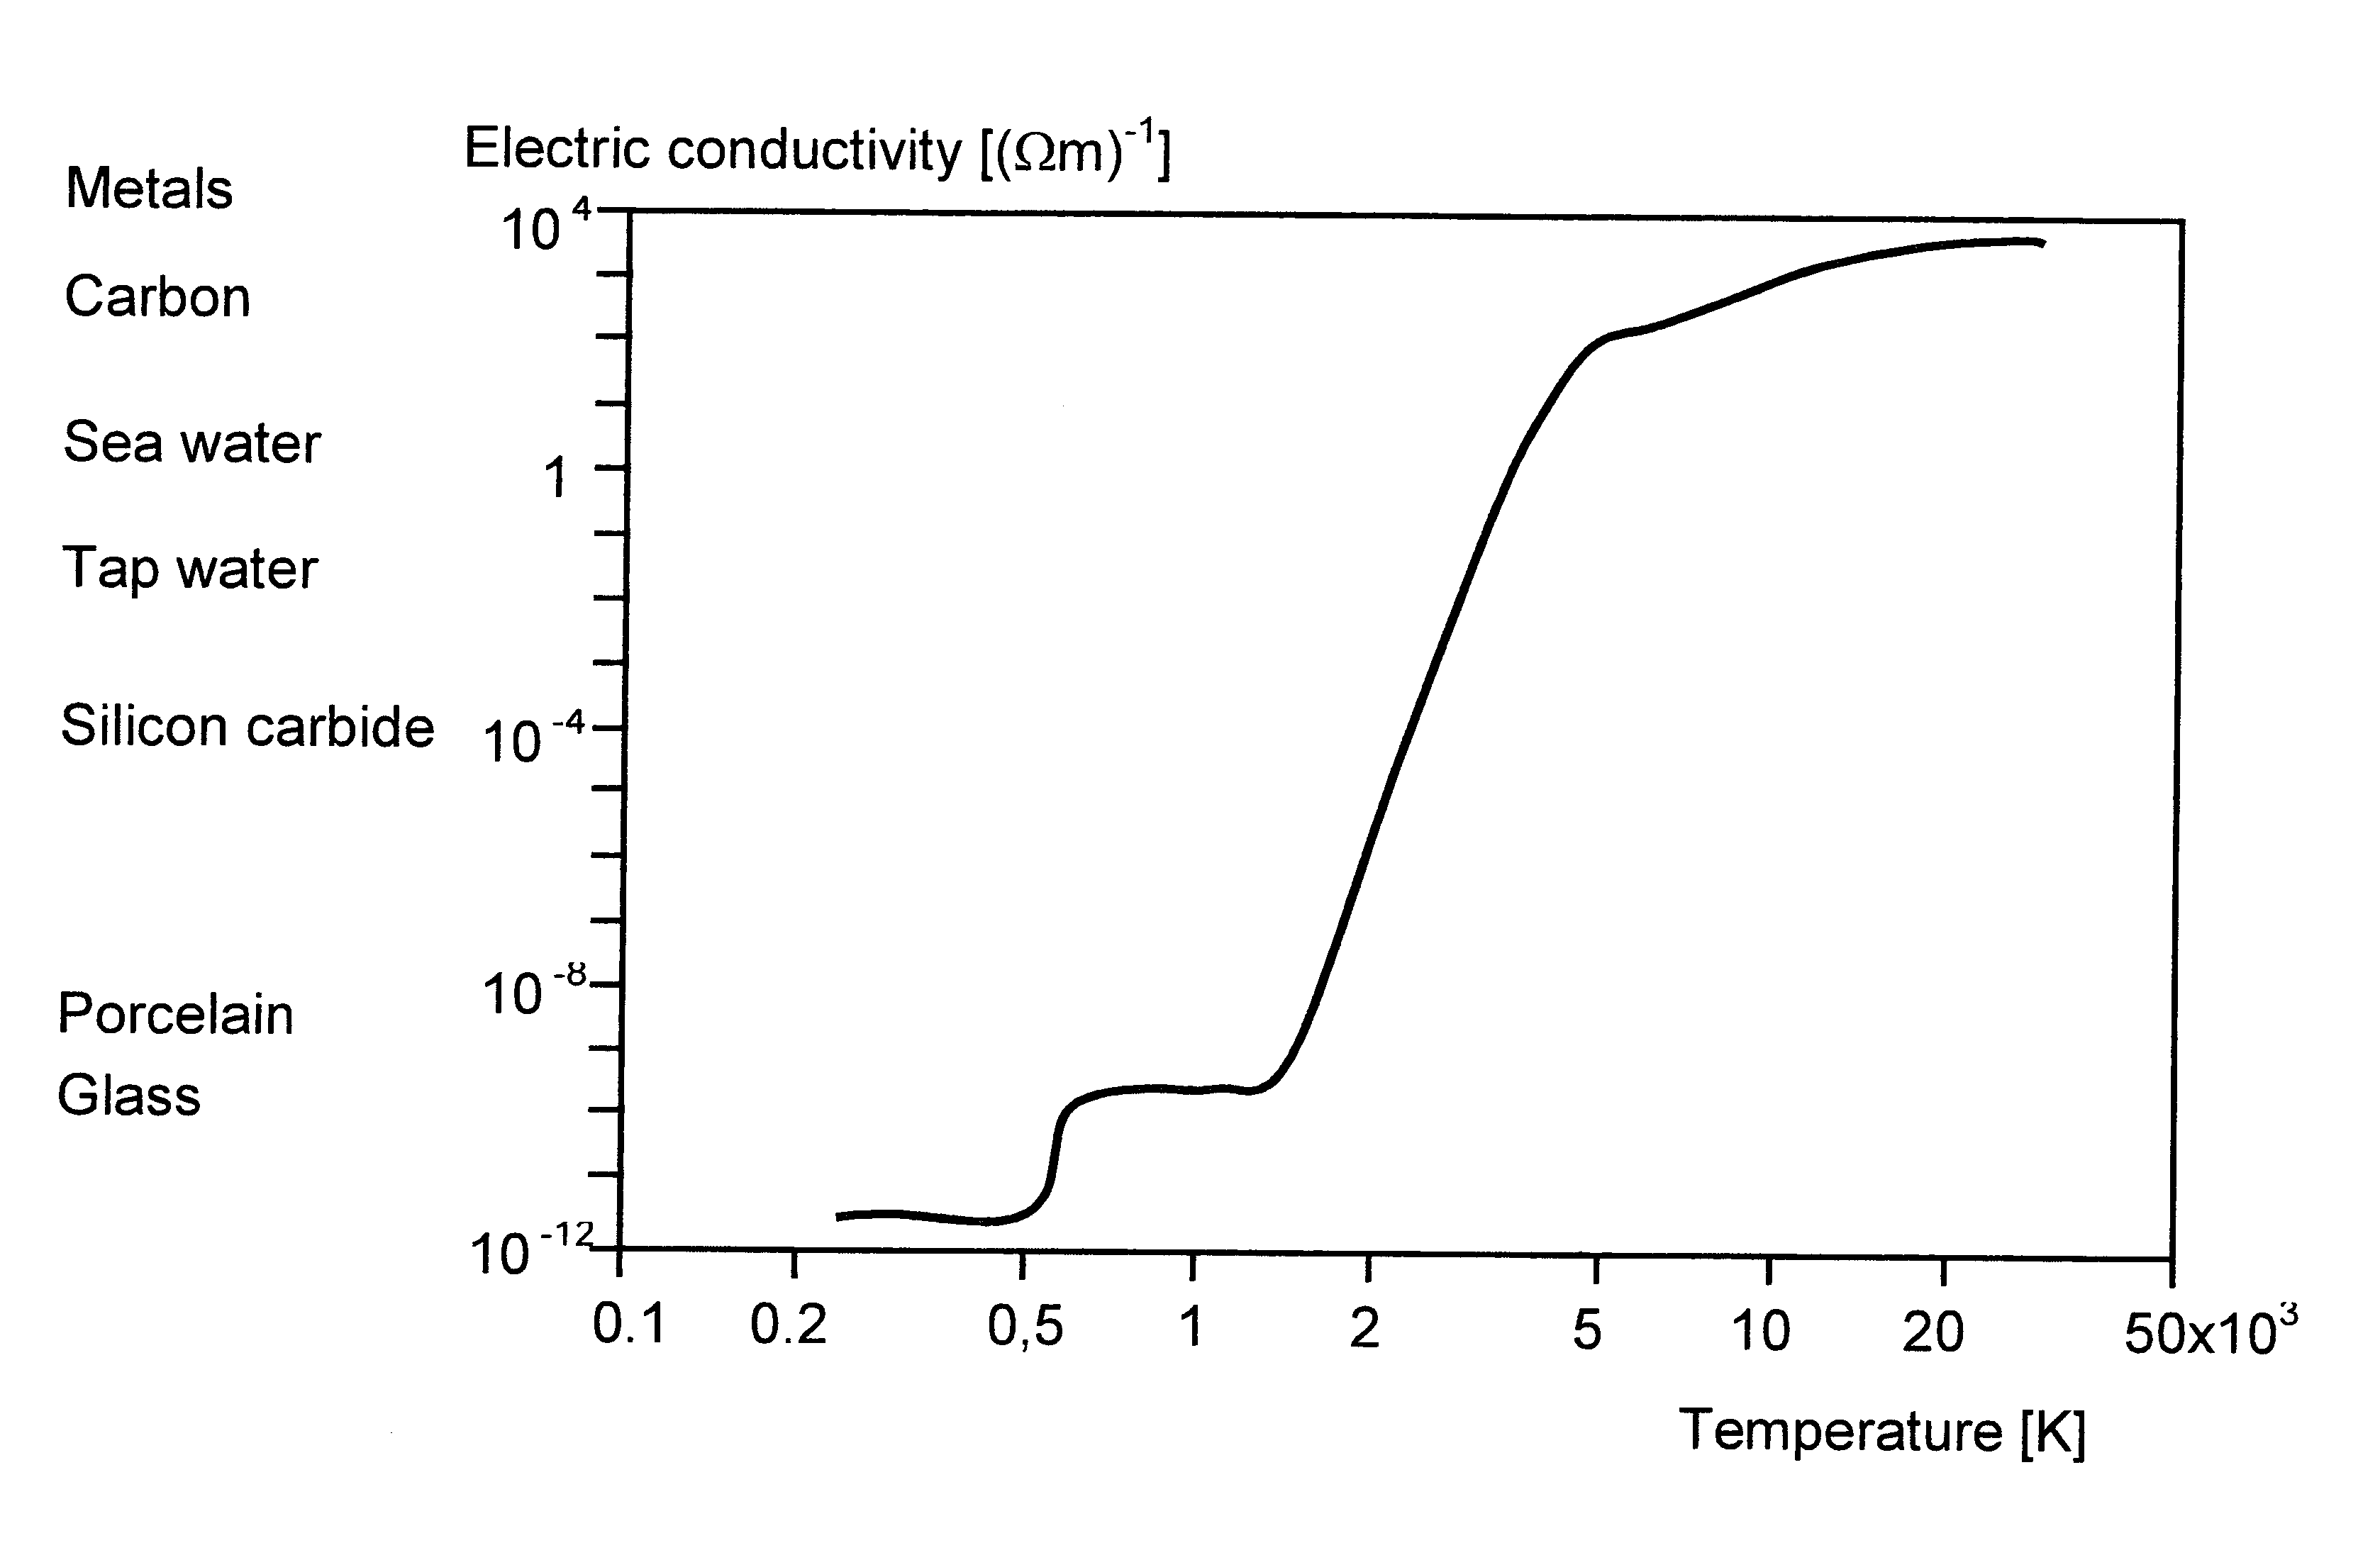
\includegraphics[scale=0.9]{Bilder/Theory/airConduct.png}
\caption{Electrical conductivity of air at atmospheric pressure \cite{bib:HVEbreak}.} \label{fig:condAir}
\end{figure}

The steep increase in conductivity can mainly be explained by the dissociation process and ionisation of N$_2$ due to temperature increase. The particle density of nitrogen as it dissociates due to high temperature in the gas is illustrated in figure \ref{fig:Ndensi}. When figure \ref{fig:Ndensi} is compared to figure \ref{fig:condAir}, a connection between temperature and the rapid decline of N$_2$, generation of the positive ion N$^+$, and the steep increase in conductivity of air is clearly visible.

\begin{figure}[H]
\centering
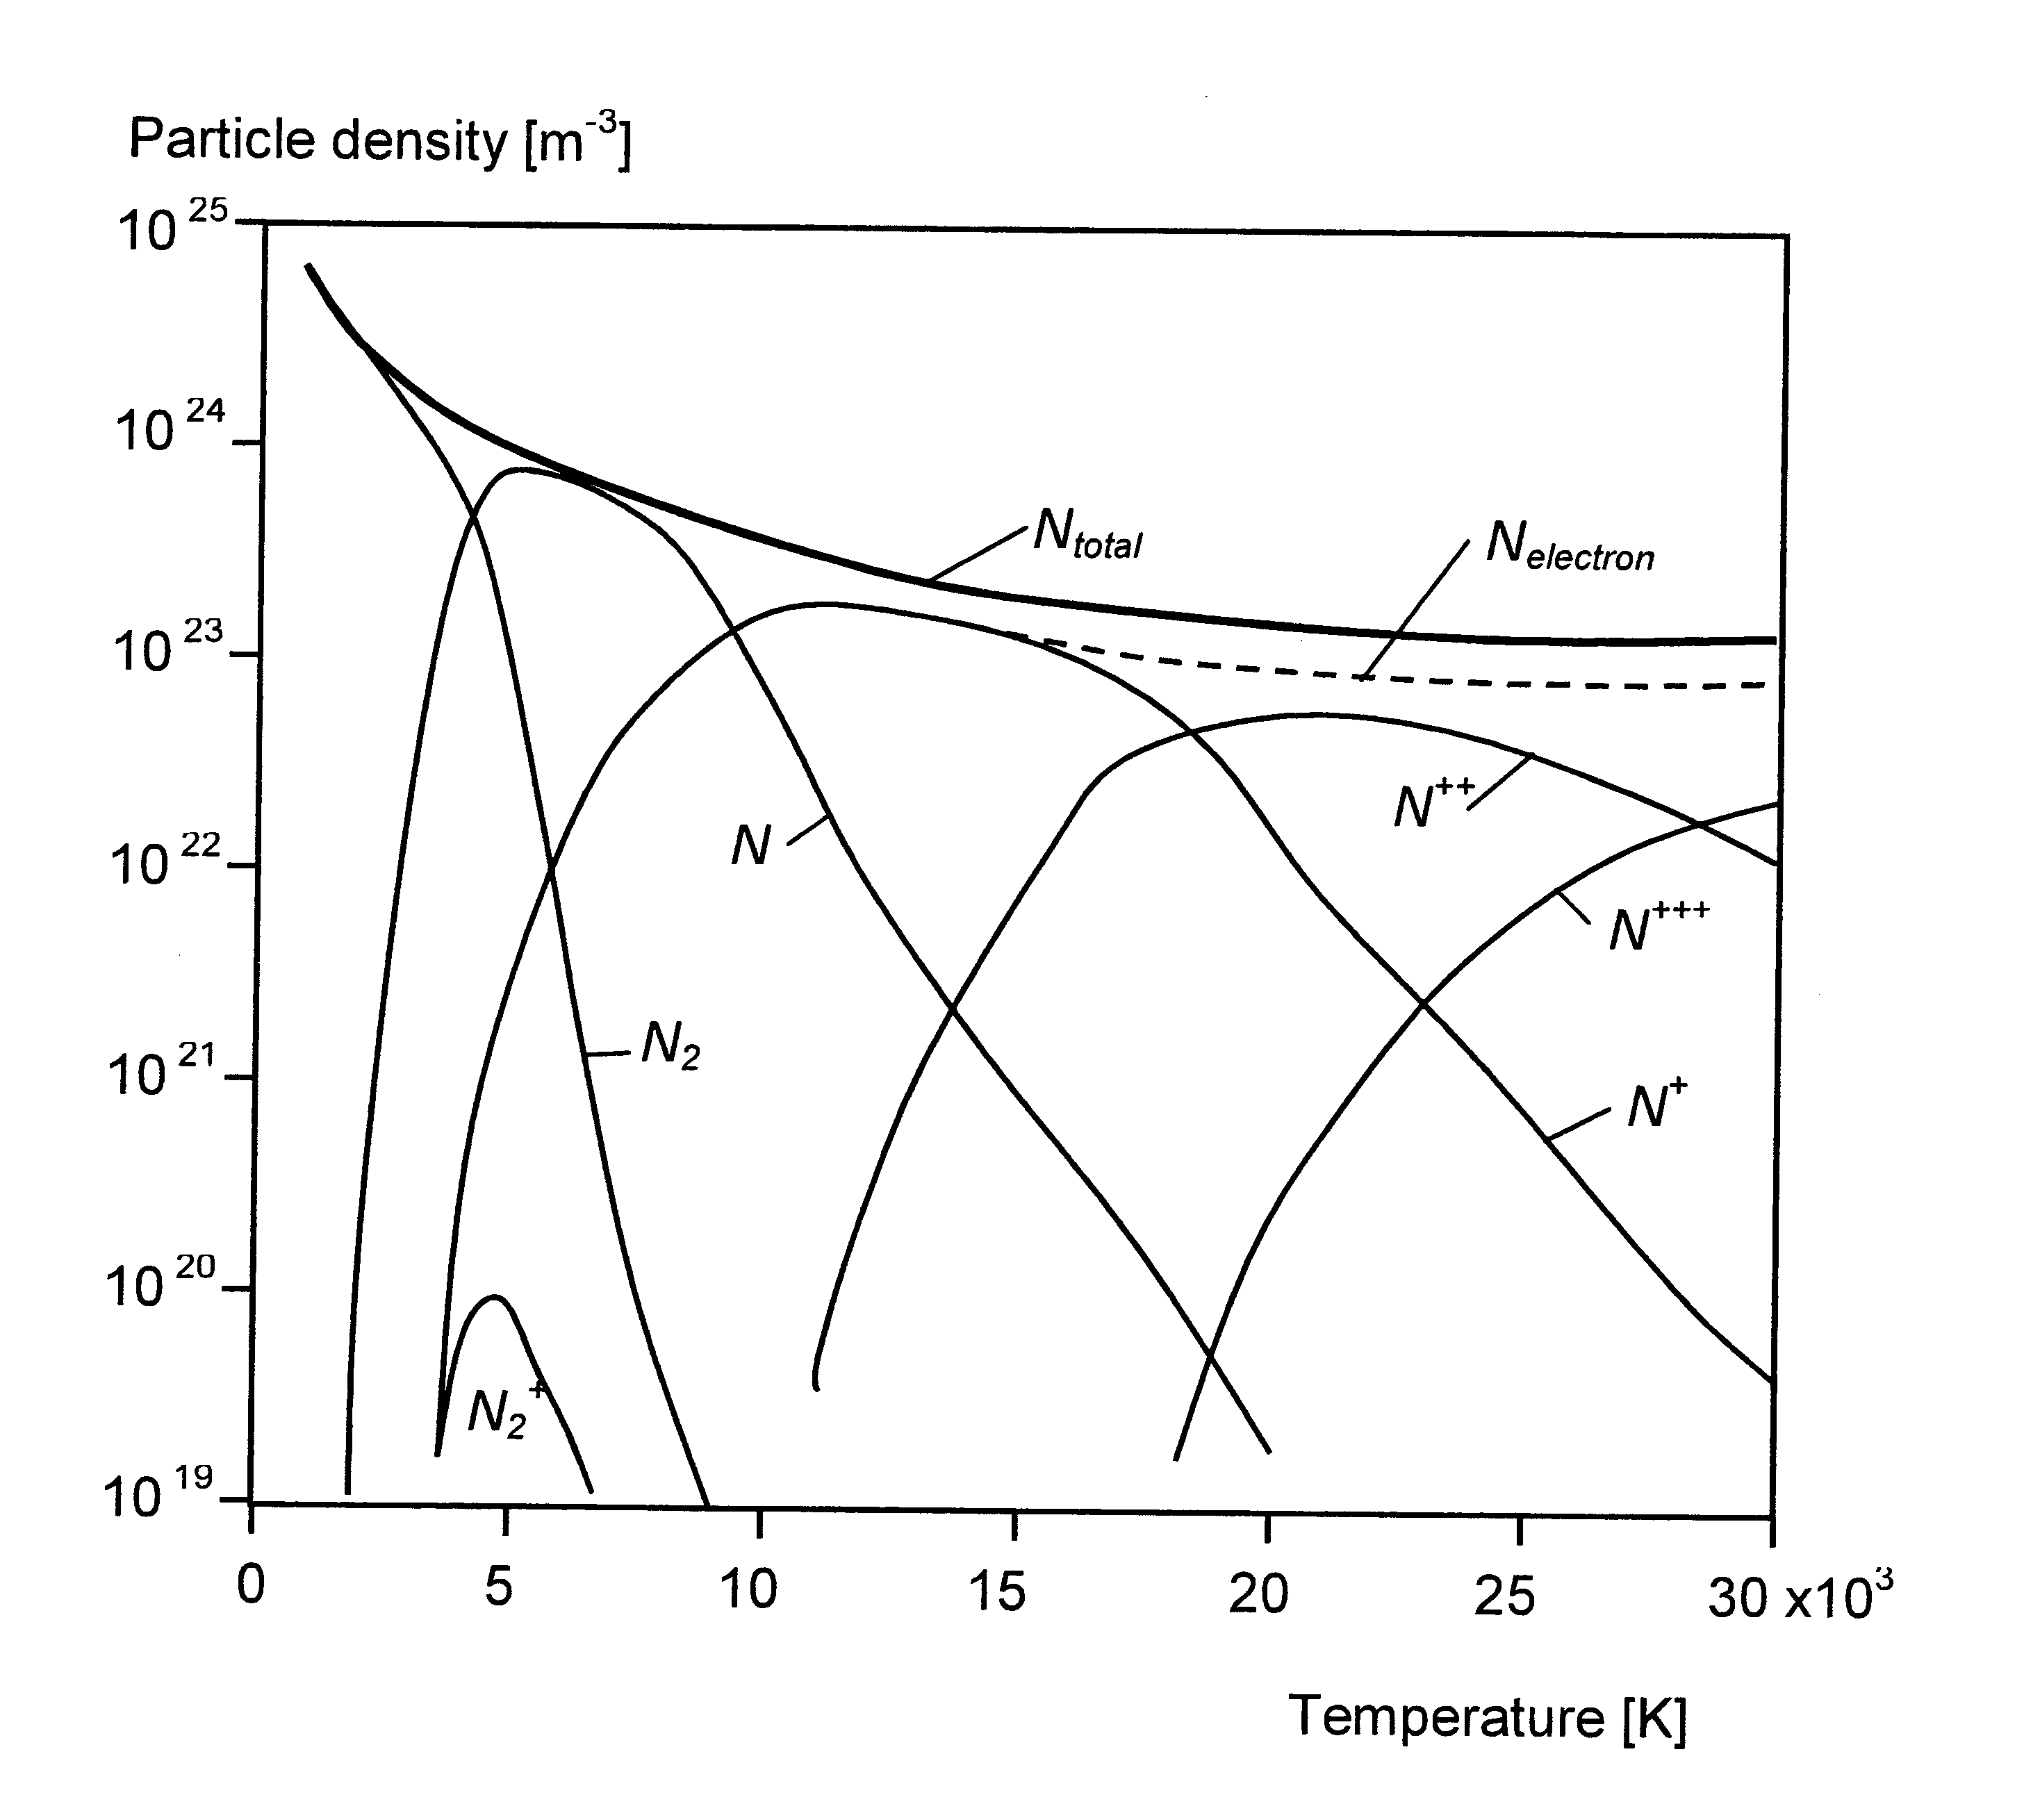
\includegraphics[scale=0.8]{Bilder/Theory/particleDensNit.png}
\caption{Particle density for different dissociation and ionisation products of nitrogen as a function of temperature \cite{bib:HVEbreak}.} \label{fig:Ndensi}
\end{figure}

Nitrogen is an electropositive gas, which means that it will have a tendency to give away electrons from its outer shell easily, especially when a strong electric field is applied and the gas is subjected to high temperatures. From figure \ref{fig:Ndensi}, the electropositive effect of N$_2$ is indicated via the generation of N$_{2}^{+}$ molecules. This reduces the breakdown voltage of the gas. From table \ref{tab:thermalIonisation}, the thermal ionisation energy for some gases is presented. This points out that N$_2$ has a significant lower ionisation energy than SF$_6$, and therefore gives away electrons more easily.

\begin{table}[H]
\center
\caption{Thermal ionisation energy for some gases \cite{bib:HVEbreak}.}
\begin{tabular}{|l|c|c|}
\hline 
Particle type & Single ionisation [eV] & Double ionisation [eV] \\ 
\hline 
Air & 16.3 &  \\ 
\hline 
N$_2$ & 15.8 &  \\ 
\hline 
N & 14.5 & 44.1 \\ 
\hline 
O$_2$ & 12.5 &  \\ 
\hline 
SF$_6$ & 19.3 &  \\ 
\hline 
S & 10.4 & 33.8 \\ 
\hline 
F & 17.4 &  \\ 
\hline 
\end{tabular} 
\label{tab:thermalIonisation}
\end{table}

During a interruption sequence, it is preferred to have different electrical conductivity of the interruption gas, depending on the current magnitude. When the current magnitude is high or raising, a good conductivity is needed. For most gases, including air, this is obtained because the gas is heated by the current passing through it, resulting in a high temperature and a good conductivity. This is important for an interruption medium, as a low electrical resistance results in smaller losses, and therefore less heat generation of the surroundings. However, at the moment of CZ and after, a fast transaction from a conducting to an insulating state of the interruption gas is important, as this will avoid a re-ignition of the arc. At this stage, the interruption gas will use some time to recombine, due to both cooling and relatively slow movement of the particles the gas consists of. In addition to these effects, there will be free electrons in the contact gap, which increases the re-ignition chance. The oxygen in air is highly electronegative and will capture electrons. However, the concentration of oxygen is small relative to the concentration of nitrogen in air, and the electronegative effect is overall weak. Because of this, a puffer is used to blow away the charged particles and hot gas between the electrodes to avoid a re-ignition.

\subsubsection{Heat transportation in an arc} \label{sec:HeatTransport}
There are several different thermal conduction mechanisms in an electrical arc. The efficiency of these mechanisms varies with temperature, and therefore the heat transport in the arc is strongly dependent upon the temperature. In figure \ref{fig:tempConGas}, the thermal conductivity of several common interrupting gases as a function of temperature is compared.

\begin{figure}[H]
\centering
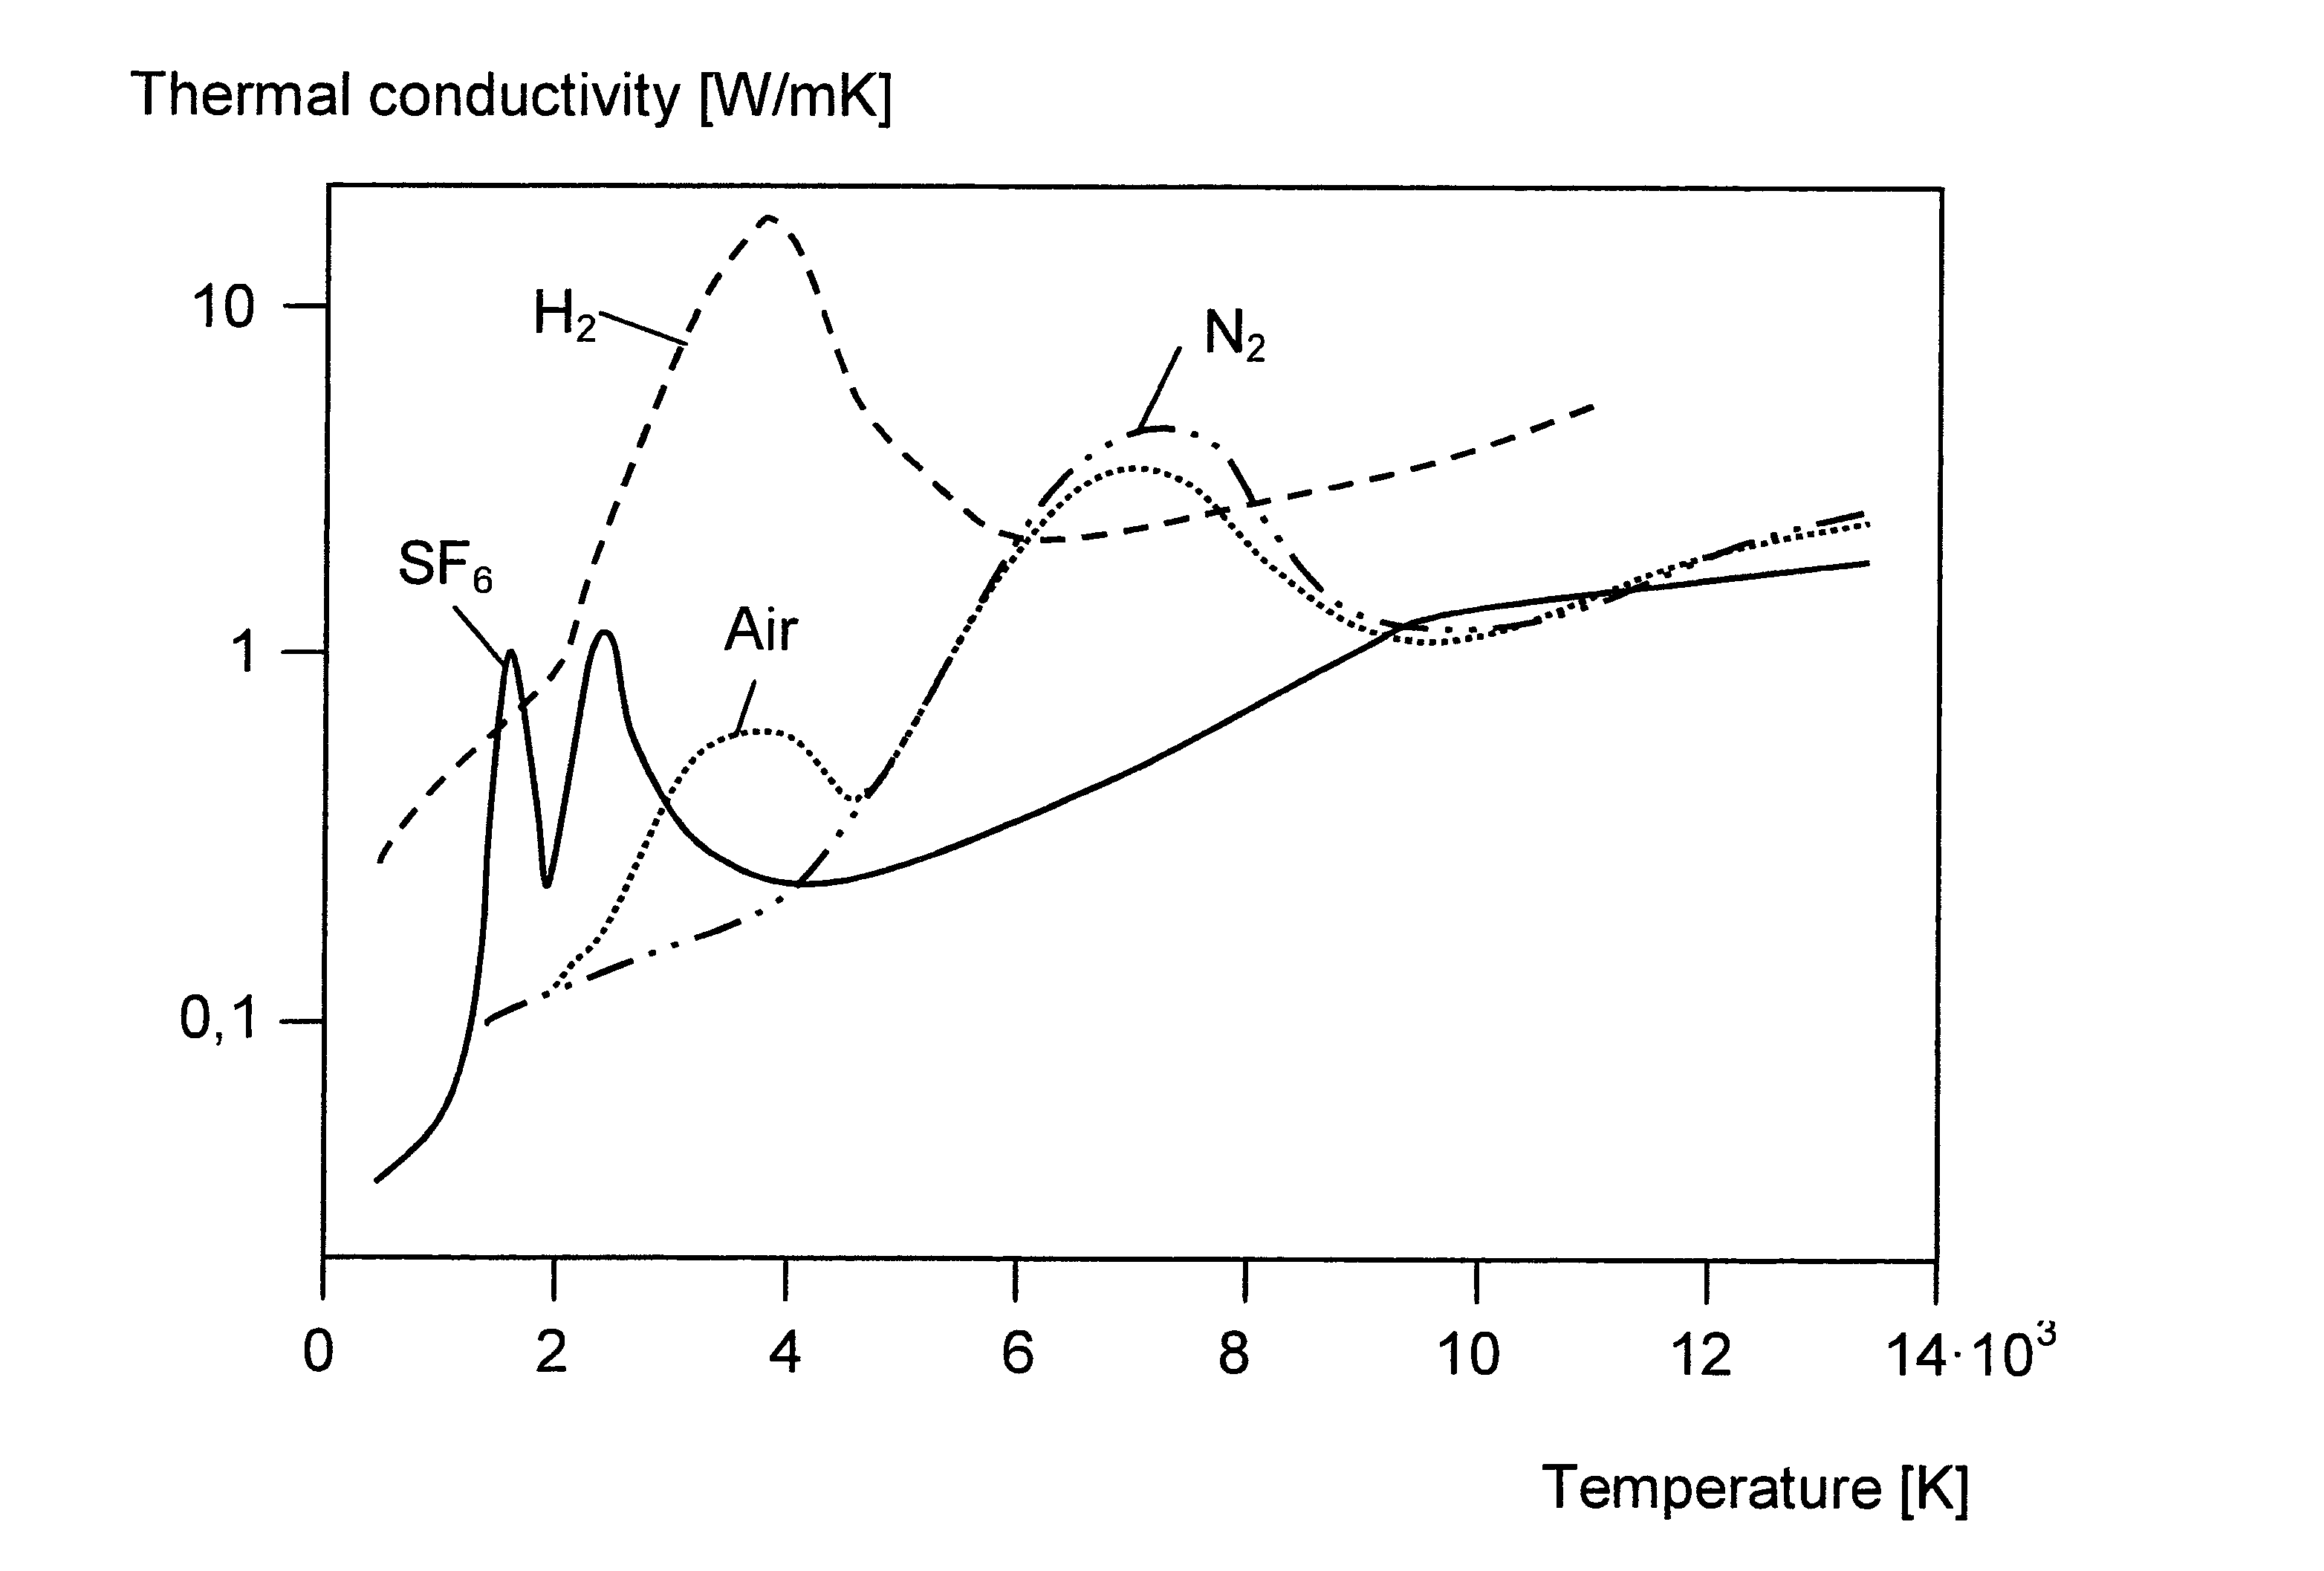
\includegraphics[scale=0.83]{Bilder/Theory/thermalCond.png}
\caption{Thermal conductivity for various gases as a function of temperature \cite{bib:HVEbreak}.} \label{fig:tempConGas}
\end{figure}

Due to the nature of the different stages of the current interruption process, it is desirable to use a gas that has a thermal conductivity that suits the different stages. When the current amplitude is rising, or is high, it is preferred that the thermal conductivity is low. This means that the plasma channel does not heat its surroundings, but mainly keeps the dissipated energy stored in its core. This will result in a huge temperature rise in the plasma channel and a relatively small increase in the surroundings. As explained in section \ref{sec:eleCondArc}, a high arc temperature will result in high conductivity in the arc, which gives a low arcing voltage. If the thermal conductivity is high in this region, more heating of the surrounding system will occur. This might result in a slower transition between the conductive and insulating stage of the interrupting medium, due to the stored energy in the medium and the surroundings, resulting in a higher chance of re-ignition.

At the moment right before CZ, it is an advantage if the thermal conductivity of the gas is high. This will result in a fast cool-down time of the plasma channel, since both the current amplitude is decreasing and the energy stored in the arc now is released to its surroundings. A gas with high thermal conductivity in this stage of the interruption process will be able to recombine from an ionised and highly conductive to a non-conductive state fast, making it more difficult for a thermal re-ignition to occur. This is because of the quick cooling of the plasma channel. In gases where the thermal conductivity is low, the cooling mechanisms are of great importance, since a quick recombination of ionised gas does not occur in the same manner as when the medium is quickly cooled. Therefore, removal of hot gas and charge carriers must be done differently. This is described in detail in section \ref{sec:genDes}. The thermal conductivity profile of air is not well suited for current interruptions, at least compared to the one of SF$_6$. If figure \ref{fig:tempConGas} is consulted, it can be observed that air has a high conductivity when the temperature is high, and a low conductivity when the temperature is low. This is the opposite of the preferred characteristics. Even though air has a small peak in thermal conductivity between 3000 K and 4000 K, its thermal conductivity profile is regarded as one of the major challenges when using air as an interruption gas. 

The temperature distribution in a plasma channel can be divided into three regions \cite{bib:TDCIGBB}, as illustrated with figure \ref{fig:tempDist1}. Zone 1 is the highly conductive arc core and also the zone with the highest temperature. Zone 2 acts as an energy buffer during the decay of the arc, while zone 3 is the cold gas surrounding the arc. When using cooling-mechanisms to quench the arc, it is primarily the second zone of the temperature profile that is cooled. The first zone's temperature will mainly be dependent on the current passing through the arc, and will not be influenced by the cooling mechanism to the same degree. If the cooling is sufficient, the energy stored in zone 2 when the arc approaches CZ is low, and therefore its effect as an energy buffer is reduced, resulting in a rapid decline in temperature in the arc core as the current approaches zero. This makes the interrupting medium's ability to transport energy important when investigating efficient cooling methods. As figure \ref{fig:tempConGas} points out, SF$_6$ has the ability to transfer heat between zone 1 and 2 fast in the correct temperature range compared to the interrupting sequence. Air has to a lesser degree the ability to do this.

\begin{figure}[H]
\centering
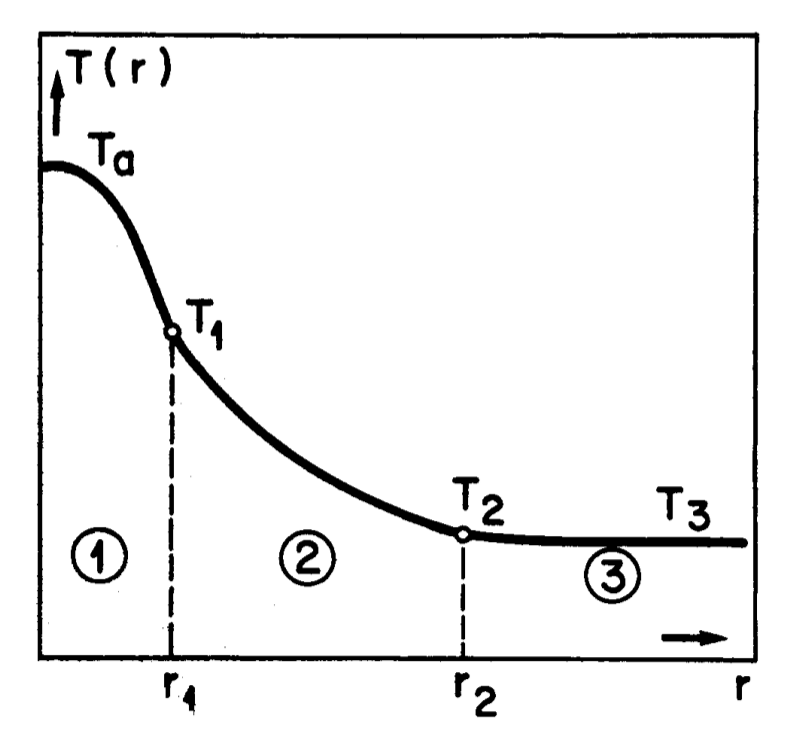
\includegraphics[scale=0.25]{Bilder/Theory/tempZonesArc.png}
\caption{Radial temperature distribution in a plasma channel (schematically) \cite{bib:TDCIGBB}.} \label{fig:tempDist1}
\end{figure}

Figure \ref{fig:tempDist2} shows how the temperature distribution varies with the electrical current. Due to radiation losses in the arc, the temperature has an upper limit of about 20 000 K to 30 000 K. At this point the cross-section of the arc will increase, rather than the temperature. However, it is not common for an LBS to experience these temperature ranges, and its temperature distribution will mainly be in the lower current ranges of figure \ref{fig:tempDist2}.

\begin{figure}[H]
\centering
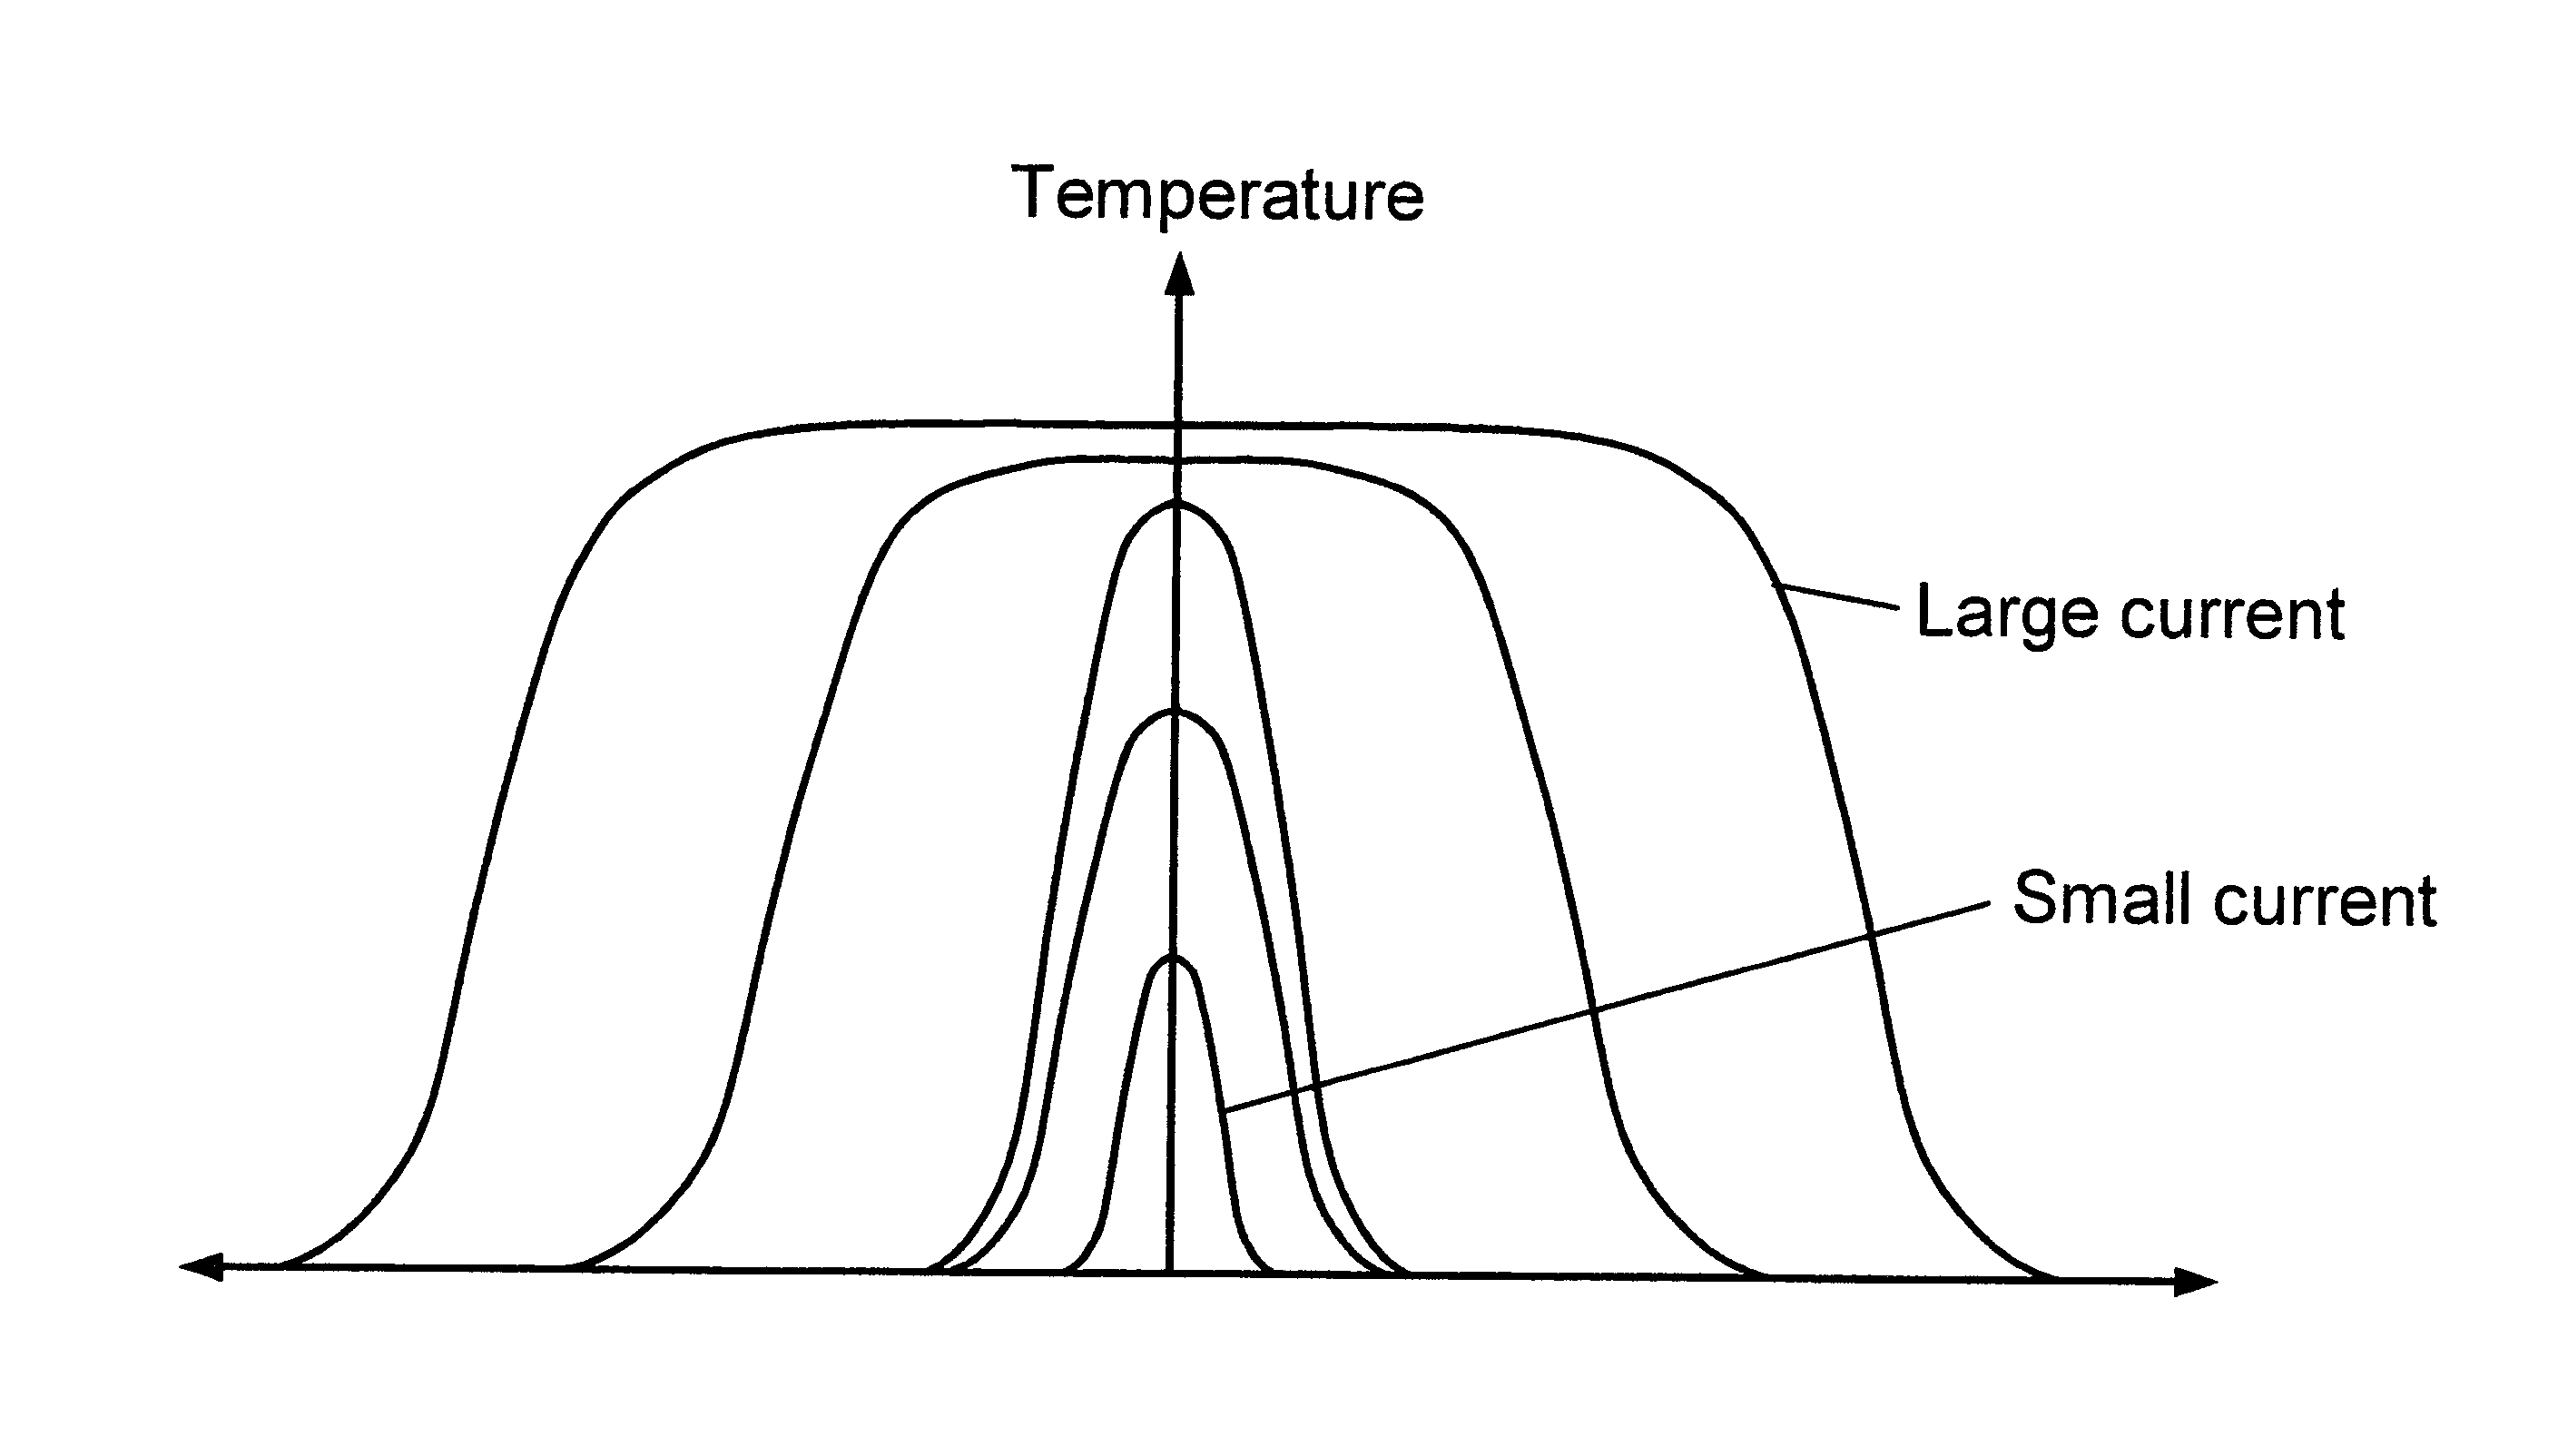
\includegraphics[scale=0.85]{Bilder/Theory/plasmaChannel1.png}
\caption{The radial temperature distribution in a plasma channel for different current magnitudes (schematically) \cite{bib:HVEbreak}.} \label{fig:tempDist2}
\end{figure}

\newpage
\subsection{Arcing voltage}
Most of the information in section \ref{sec:genDes} is collected from \textit{"Current Interruption in Power Grids"} by Magne Runde \cite{bib:HVEbreak} \newline

\subsubsection{Static arcing voltage} \label{sec:staticArcVoltage}
It is common to distinguish the description of the arc into two different types. The most relevant and realistic is called a dynamic arc, the other a static arc. A static arc can only be established when using DC current, and after any transients have died out. Therefore, static arcs are uncommon, and in nearly all switching operations the properties of the arc are best described by the dynamic arc model.

AC currents always generate a dynamic arc. This is because the current vary with time, and thereby the properties of the arc. In cases where DC current is used, but external factors like cooling varies over time, like in a puffer based switchgear, the arc is dynamic. When dealing with AC switchgear with a puffer based interruption method, the arc is always a dynamic arc. Due to the complexity of a dynamic arc, it is common to regard the arc to behave like a static arc within a certain time interval, and therefore some properties of a static arc will be described in this section. Dynamic arcs will be featured further in section \ref{sec:dynARC}.

The static arc characteristic is illustrated in figure \ref{fig:staticArcChar}. This describes the relationship between current and arcing voltage in a static arc. The scaling of the axes is only approximate and may vary with gas type and electrode material.

\begin{figure}[H]
\centering
\includegraphics[scale=1]{Bilder/Theory/staticArcChar.png}
\caption{Static arc characteristic (schematically) \cite{bib:HVEbreak}.} \label{fig:staticArcChar}
\end{figure}

As can be seen from figure \ref{fig:staticArcChar}, the characteristic is highly non-linear. At low currents, like tens of amperes, the voltage drop across the arc decreases with increasing current. Then the voltage is constant, and apparently independent from the current flowing in the arc. How large, and in which current range the constant part of the arcing voltage occurs, depends highly on which gas the arc burns in. For currents above this range, the arcing voltage begins to increase with the current.

In figure \ref{fig:potDisArc}, the potential distribution of an electrical arc is illustrated. A static electrical arc might be regarded as divided into three regions:

\begin{description}
\item[Cathode region:] The voltage drop, $\mathrm{V_c}$, is typically some 20 V.
\item[Arc column:]	There is a constant electric field in this region, typical 1 V/mm.
\item[Anode region:] The voltage drop, $\mathrm{V_a}$, is typically some 3 V.
\end{description}

\begin{figure}[H]
\centering
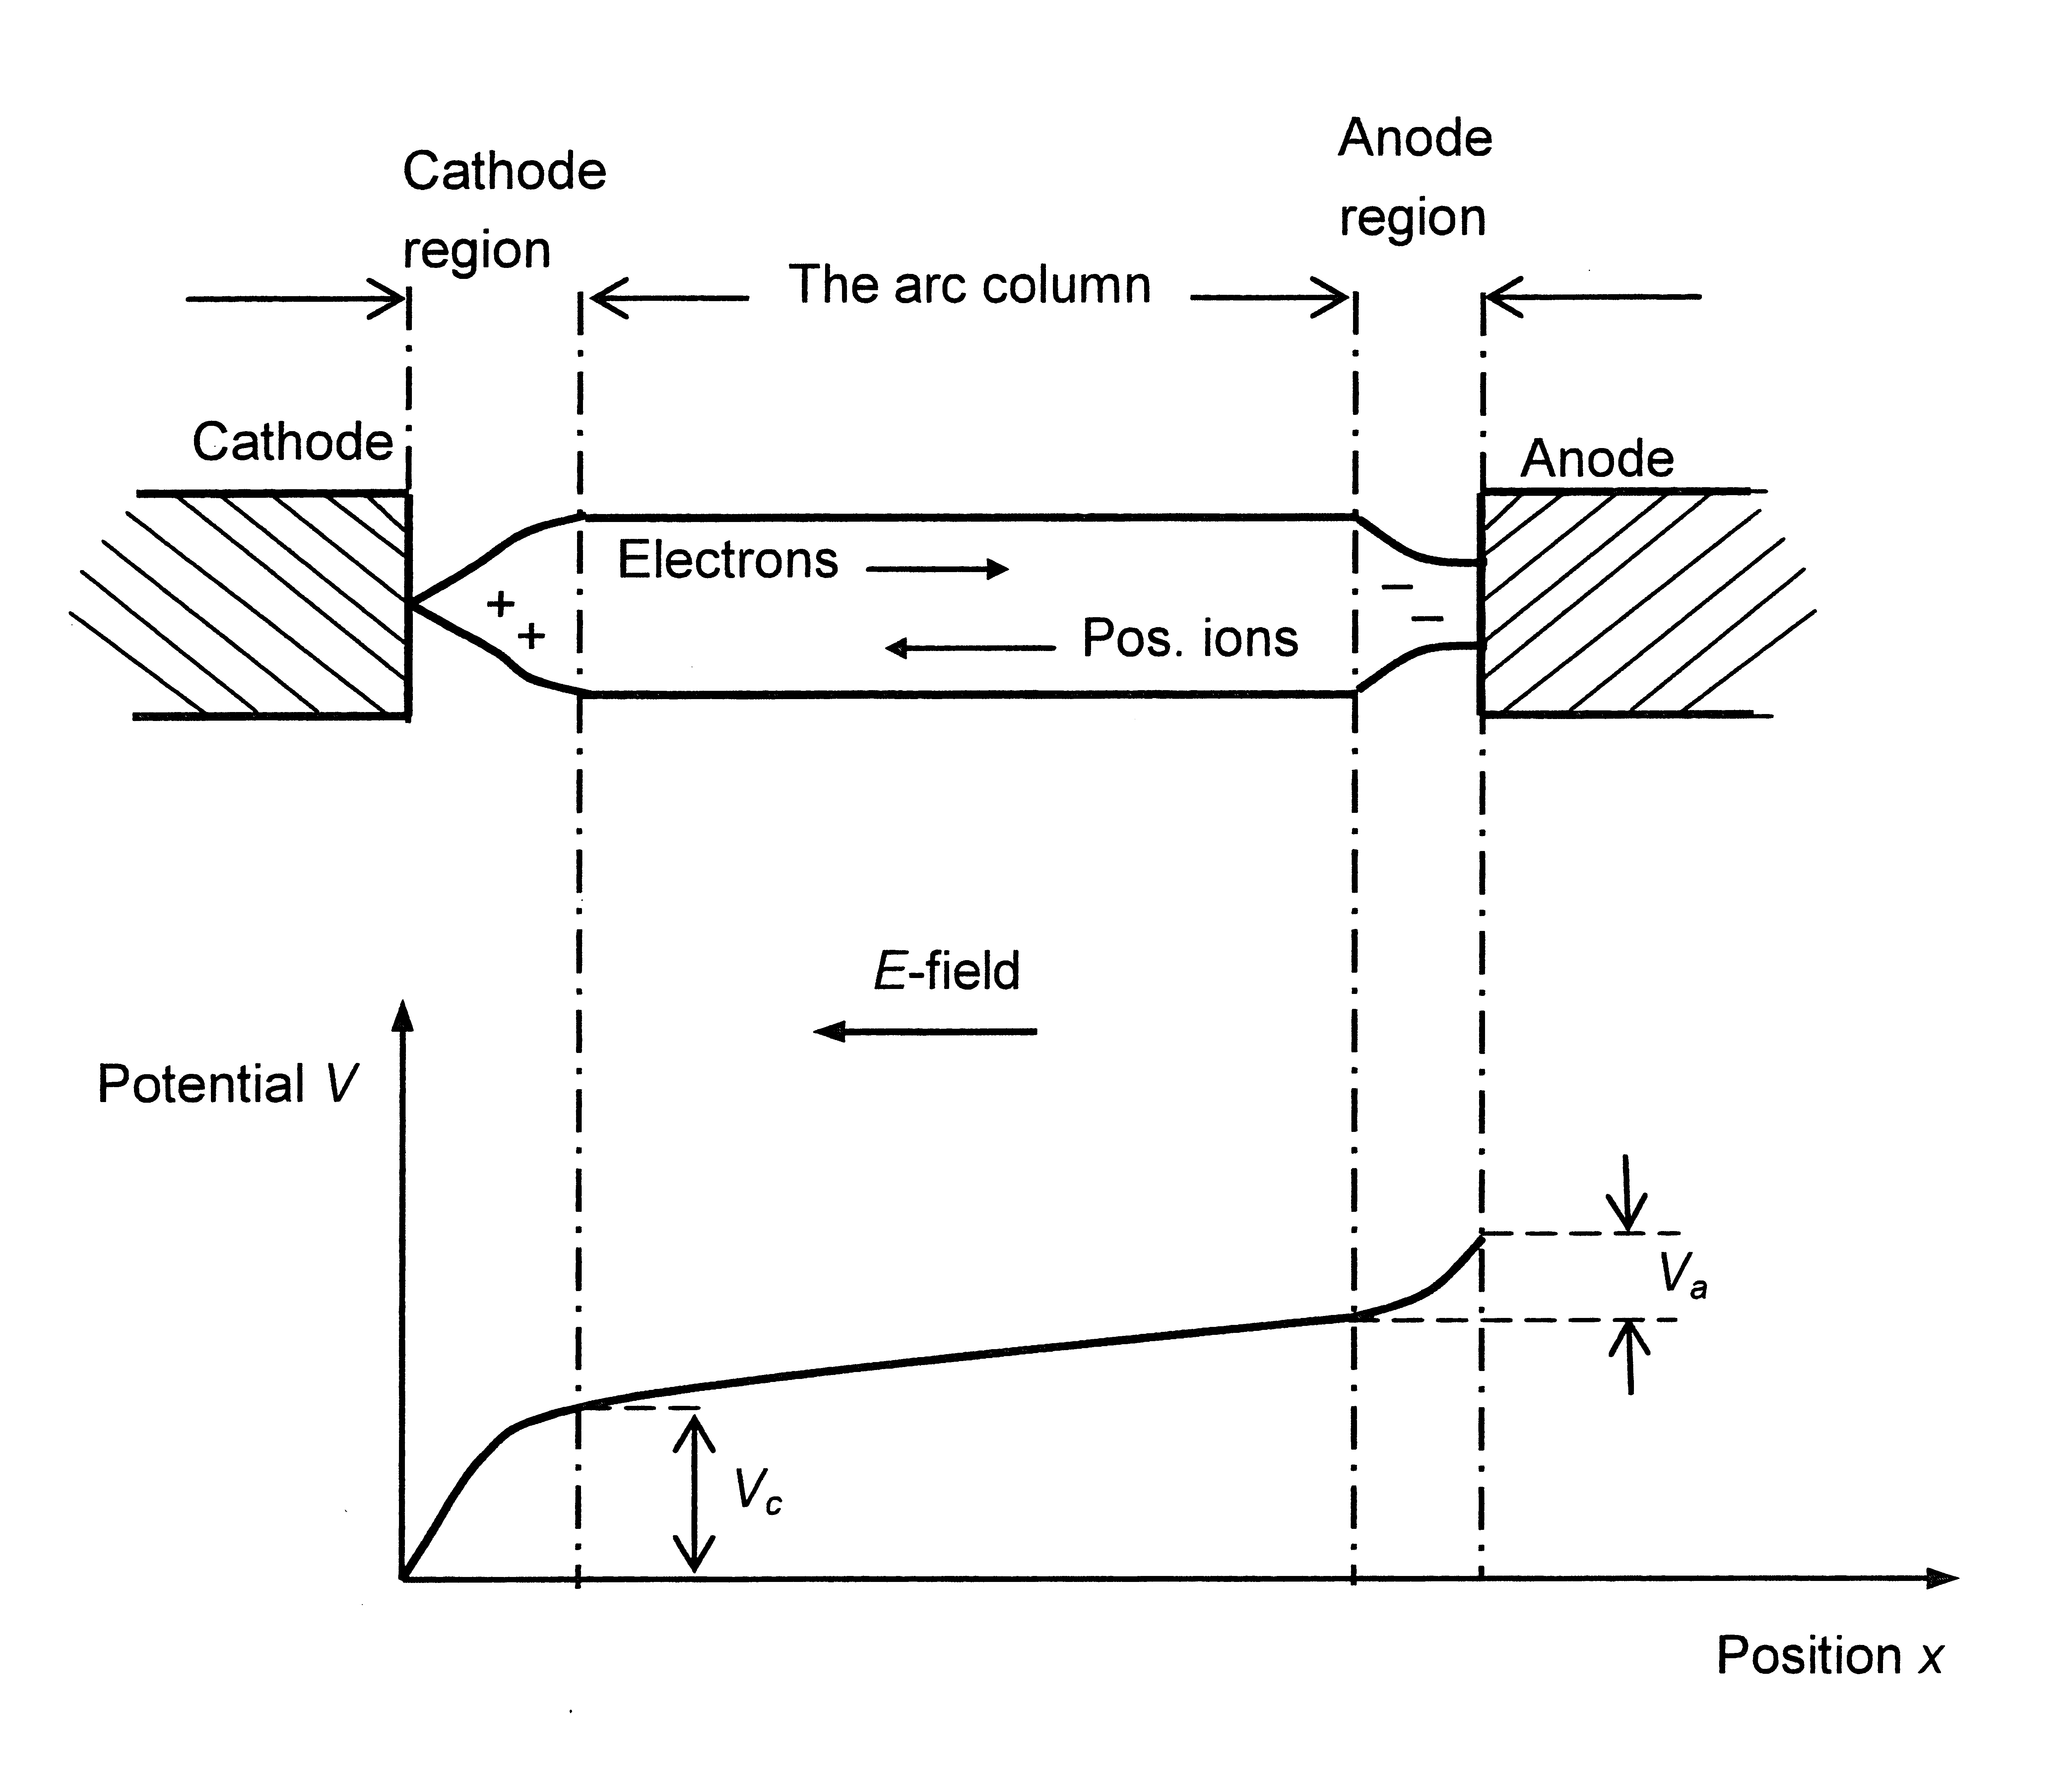
\includegraphics[scale=0.8]{Bilder/Theory/potentialDistArc.png}
\caption{Cross-section of a stationary arc and the corresponding potential distribution (schematically) \cite{bib:HVEbreak}.} \label{fig:potDisArc}
\end{figure}

The description above is highly general, and the voltage distribution will vary depending on which gas the arc is burning in, as well as the current range and the electrode materials being used. Therefore, the potential distribution across a dynamic arc that burns in air for a typical current range of an LBS is analysed. The analysis is based on results from previously conducted tests performed with the test circuit presented in section \ref{sec:testCir}. Three interruption test, where a thermal re-ignition occurred after the first CZ and the second CZ, are selected. The pressure in the pressure chamber was held constant throughout the whole test, and was set to 1.0 bar upstream pressure. The RMS value of the current was 630 A, while the contact and nozzle geometry was the same for each of the three tests. In figure \ref{fig:threeTests}, the arcing voltage during the three chosen interruption tests is shown.

\begin{figure}[H]
\centering
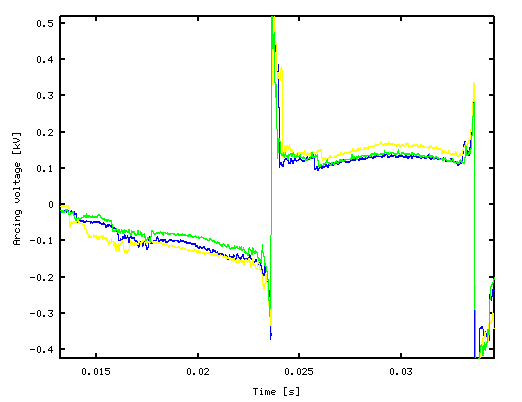
\includegraphics[scale=0.7]{Bilder/Theory/threeTests.png}
\caption{Arcing voltage during three interruption tests. The y-axis is arcing voltage in kV and the x-axis is time in seconds from test start.} \label{fig:threeTests}
\end{figure}

The average arcing voltage from these three tests is presented in figure \ref{fig:averageArcingVoltage}, and it is applied to approximate the potential distribution of the burning arc.

\begin{figure}[H]
\centering
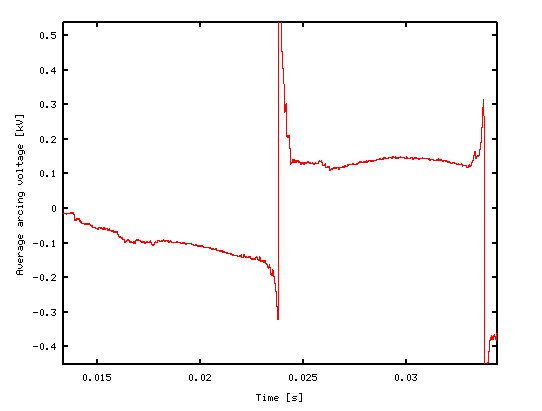
\includegraphics[scale=0.7]{Bilder/Theory/averageOfthreeTests.png}
\caption{Average arcing voltage for three interruption tests. The y-axis is arcing voltage in kV and the x-axis is time in seconds from test start.} \label{fig:averageArcingVoltage}
\end{figure}

In both figure \ref{fig:threeTests} and \ref{fig:averageArcingVoltage}, contact separation occurs at $t \approx 0.0140$ s. The first CZ occurs at $t \approx 0.0235$ and the second CZ occurs at $t \approx 0.0335$ s. The arcing time that is the time from contact separation to the first CZ, is approximately 9.5 ms for all the three tests.

The length of the arc is determined by the distance between the contacts, which move apart with a constant speed of approximately 5 m$/$s. When the arc is short, most of the arcing voltage will be close to the electrodes. To establish an estimate over the voltage drop in close vicinity of the electrodes, the average voltage when the contacts were between 0.4 mm and 1.4 mm apart was calculated. Because of transients in the arcing voltage when the arc ignites, a contact gap length less than 0.4 mm was unsuited for this use. Due to the short length of the arc in this time span, the average arcing voltage in this region can represent an approximation of the voltage drop close to the electrodes. This voltage drop is estimated to 33 volts in absolute value, when using the procedure above.

Then the increase in arcing voltage per millimetre is calculated. Linear regression when the arc is between 23.2 mm and 38.8 mm is used to establish the rate of rise in the arcing voltage, and thereby the increase in arcing voltage caused by elongation of the arc can be established. This rate of rise was calculated to be 2.7 V$/$mm in absolute value.

The final expression in absolute value for the voltage across the arc, where x is the length of the arc in millimetres, then becomes:
\begin{equation}
V(x) \approx 2.7x+33 \ \ \ \ x \in [0.4, 40.0] \ \mathrm{mm}
\end{equation}

This estimation of the arcing voltage fits well in the region between contact separation and the first CZ. In the region between first and second CZ, this model is not suited. It is assumed that the values calculated here will be dependent on both upstream pressure and test current.


\subsubsection{Dynamic arcing voltage} \label{sec:dynARC}
When the current or cooling of the arc changes with time, the arcing voltage no longer follows the static arc characteristics presented in figure \ref{fig:staticArcChar}. This is because the temperature cannot change instantaneously, since it is impossible to use an infinite amount of power to heat or cool a certain mass instantaneously. This gives an arc a certain thermal inertia.

Thermal inertia causes the arc to "remember" the amplitude of the current that just passed for a short period of time. If the current follows a step function, the arc voltage will at first take a higher value, and then gradually decrease to the value corresponding to the static arc characteristic, as presented in figure \ref{fig:timeConstantStep}. This is because the arcing voltage mainly is set by the electrical conductivity of the arc, which is highly dependent on the temperature. Since the temperature cannot change instantaneously, the arcing voltage can be regarded as a function of time with approximately an exponential decay. The time constant of this decay varies from gas to gas. In table \ref{tab:timeConstants}, the time constant for some gases is displayed. The time constant for each gas depends on several factors, like test method and current magnitude. The variation of the time constant alters with the current, and can to a certain degree be compared to the inverse of the thermal conductivity's dependency of temperature presented in figure \ref{fig:tempConGas}, where the temperature is proportional to the current. 

\begin{figure}[H]
\centering
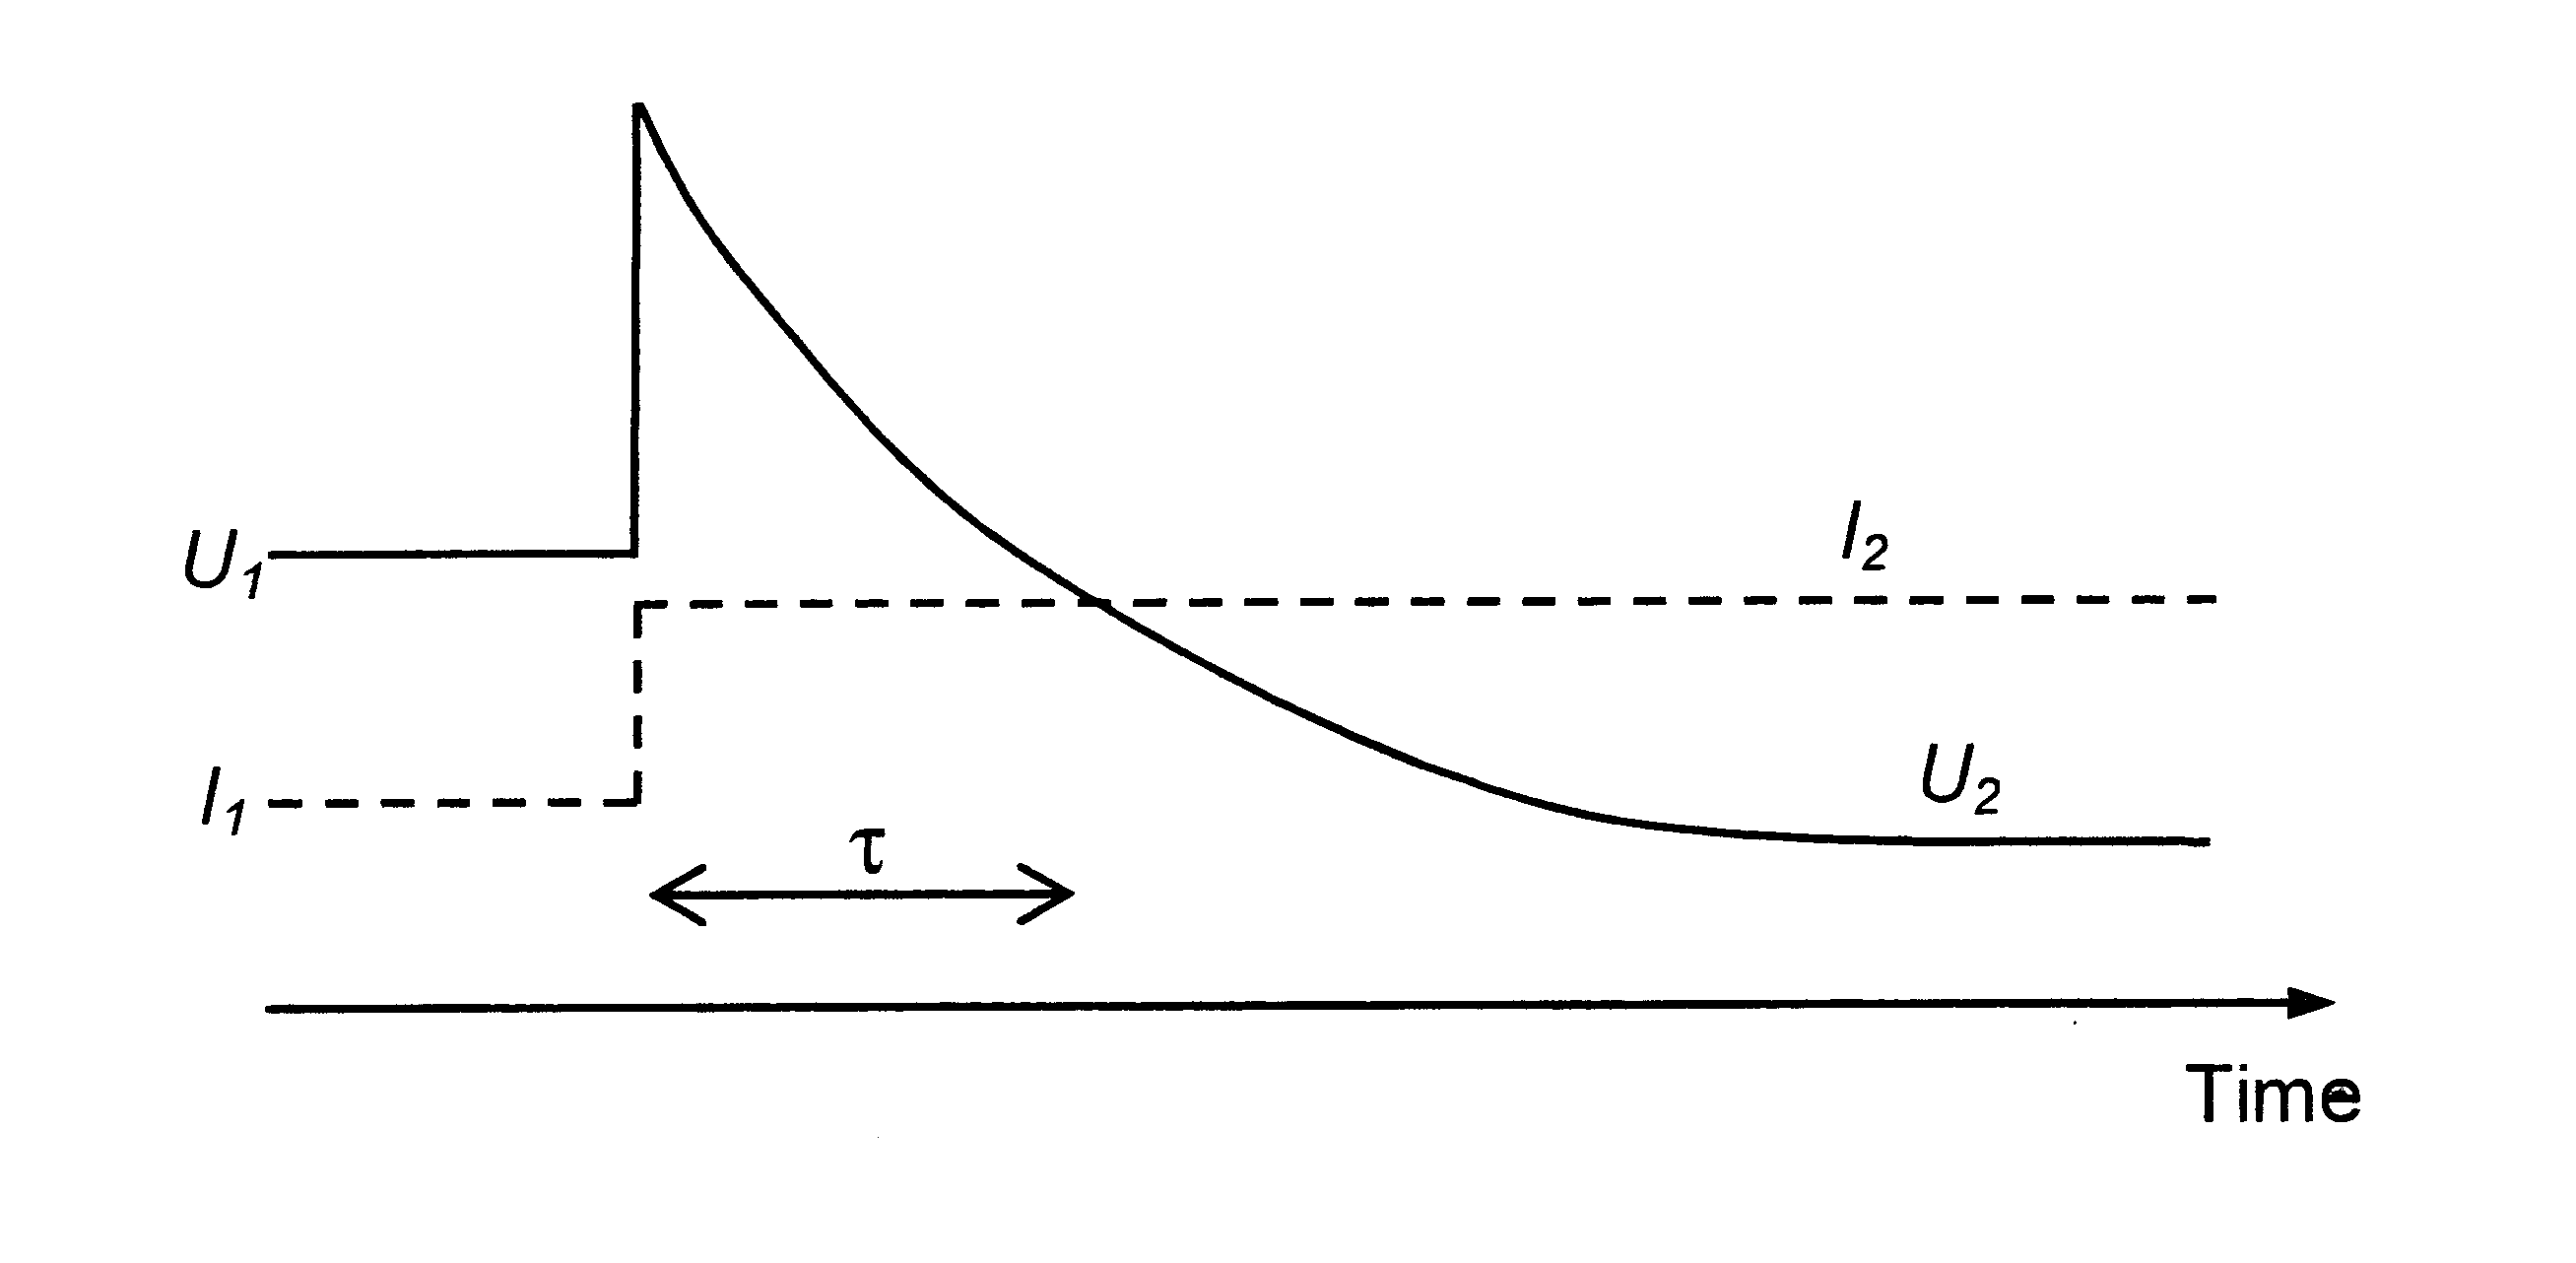
\includegraphics[scale=1]{Bilder/Theory/timeConstants.png}
\caption{Voltage drop of an arc exposed to a current that follows a step function (schematically) \cite{bib:HVEbreak}.} \label{fig:timeConstantStep}
\end{figure}

\begin{table}[H]
\center
\caption{Time constants in a 1 A arc burning in a 19 mm tube (schematically) \cite{bib:HVEbreak}. }
\begin{tabular}{|c|c|}
\hline 
Gas & Time constant [$\mu$s] \\ 
\hline 
SF$_6$ & 0.8 \\ 
\hline
O$_2$ & 1.5 \\
\hline
CO$_2$ & 15 \\
\hline
Air & 80 \\
\hline
N$_2$ & 210 \\
\hline
H$_2$ & 1 \\
\hline
\end{tabular} 
\label{tab:timeConstants}
\end{table}

A gas with a low time constant is faster to cool, and thereby reduces its electric conductivity faster than a gas with a large time constant. This is an advantage during current interruption. Air has a fairly high time constant resulting in a slower cool-down time than other interrupting gases. This is closely related to the problems mentioned in section \ref{sec:HeatTransport}. 

In figure \ref{fig:arcingVoltageFre}, the arcing voltage for a dynamic arc is illustrated. As shown by the figure, the arcing voltage varies both with current and frequency. In figure \ref{fig:arcingVoltageVSCurrent}, the arcing voltage with regard to current for a previously conducted interruption test is shown. As can be observed from this figure, the arcing voltage follows the same pattern as an dynamic arc burning at 50 Hz shown in figure \ref{fig:arcingVoltageFre}. Some differences in the burning conditions for the arc in figure \ref{fig:arcingVoltageFre} and \ref{fig:arcingVoltageVSCurrent} are present. In figure \ref{fig:arcingVoltageFre}, the arc is not cooled, and the contacts are stationary with a fixed gap. In figure \ref{fig:arcingVoltageVSCurrent}, the arc is cooled with a 1.0 bar upstream pressure, while elongated by the separation of the contacts.

\begin{figure}[H]
\centering
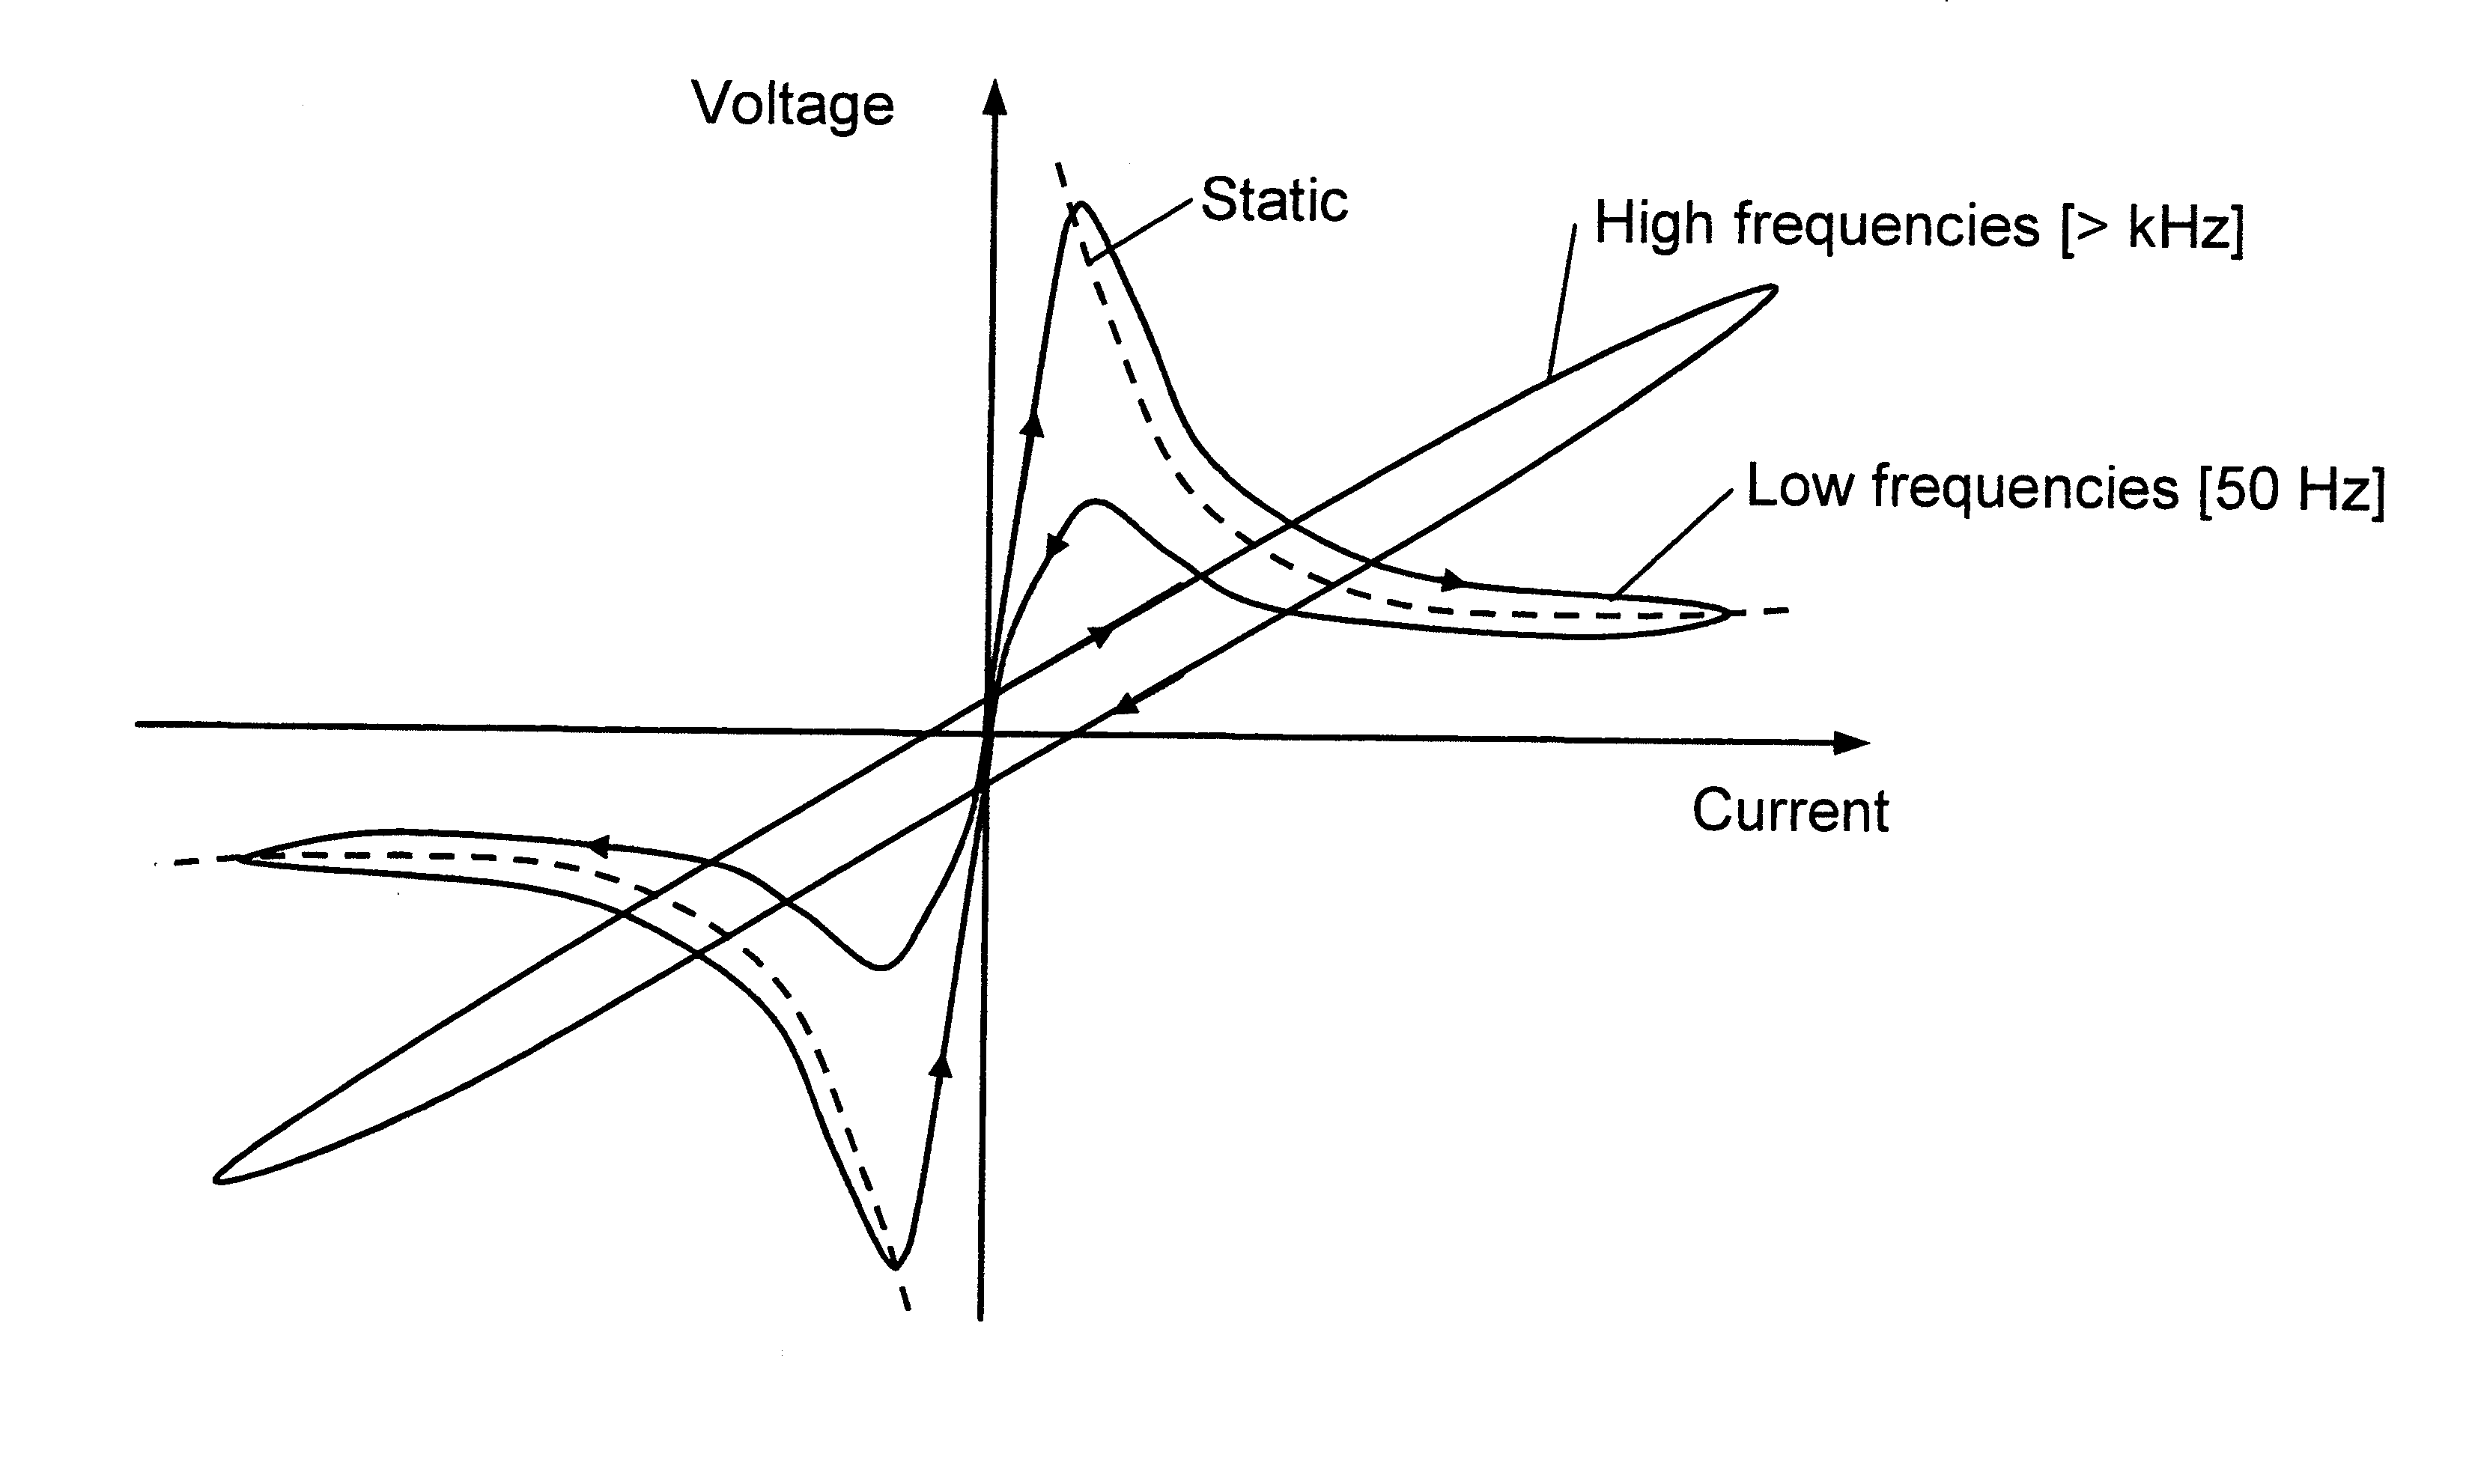
\includegraphics[scale=1]{Bilder/Theory/dynamicArcingVoltage.png}
\caption{Static, low, and high frequency arc characteristics (schematically) \cite{bib:HVEbreak}.} \label{fig:arcingVoltageFre}
\end{figure}

\begin{figure}[H]
\centering
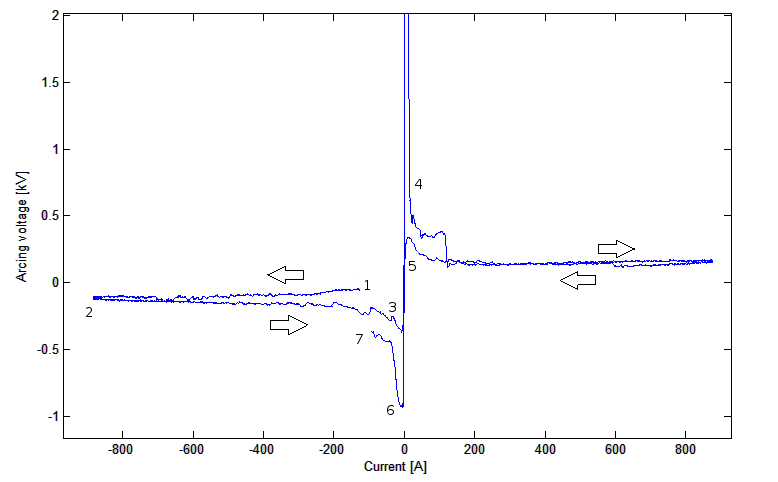
\includegraphics[scale=0.7]{Bilder/Theory/arcingVoltagevzCurrent3.png}
\caption{Arcing voltage during a full power cycle for a 50 Hz current in a test interruption.} \label{fig:arcingVoltageVSCurrent}
\end{figure}

The numbered parts in figure \ref{fig:arcingVoltageVSCurrent} represent different aspects of the arc during the interruption sequence, and are described in the list below. The arrows represent the direction of time during the interruption. A full power cycle is plotted in the figure, resulting in a time span of 0.02 seconds.
\begin{description}
\item[1:] The contacts separate and the arc ignites. As the absolute value of the current increases, the arcing voltage follows the same trend as illustrated in figure \ref{fig:arcingVoltageFre}.  
\item[2:] After the first current peak, the arcing voltage is always higher than than the corresponding arcing voltage for the same current magnitude that occurred before the current peak.
\item[3:] The arcing voltage increases as the current decreases, then at the moment of the first CZ, the arc is quenched and a high voltage peak arises.
\item[4:] Quickly after CZ, a thermal re-ignition occurs and the arc re-ignites. The high voltage peak that occurred during CZ is probably due to the intensive cooling the arc experiences. Some distortion of the arc causes the arcing voltage to drop and the pattern seen in figure \ref{fig:arcingVoltageFre} is disturbed, but the same trend can be observed.
\item[5:] The arcing voltage rises as the second CZ approaches.
\item[6:] Almost instantly after CZ, the arc re-ignites as a thermal re-ignition occurs.
\item[7:] Mainly due to elongation of the arc, the arcing voltage is higher at this point than in the beginning (point 1). If the length of the arc had remained constant throughout the whole experiment, the arcing voltage would be expected to be approximately the same at point 7 and point 1. The arc has now burnt a full power cycle, t=0.02 s, from ignition.
\end{description}

\subsection{Thermal re-ignition considerations} \label{sec:TherMalReConsid}
As mentioned in section \ref{sec:puffer}, the main purpose of the puffer mechanism is to remove charge carriers between the contacts after CZ to avoid re-ignition of the arc. After CZ, a strong electrical field rises between the electrodes, better known as the recovery voltage. This electrical field will accelerate the charge carriers in the air-gap, and the movement of these will represent a current called the post-arc current (PAC). During a high current and high voltage interruption for a circuit breaker, the peak of the PAC is usually a few amperes or less, and have a duration for some microseconds. For currents and voltages in the LBS range, the current peak of the PAC is expected to be considerably smaller.

A thermal re-ignition is avoided if the PAC reaches zero, since this means that the charge carriers in the air gap are removed. On the other side, a thermal re-ignition occurs if the PAC rises, an arc ignites, and the current obtains its common sinusoidal form. Figure \ref{fig:PACbreakandreIgnite} shows the PAC for a successful and an unsuccessful interruption in a circuit breaker when using SF$_6$ as an interrupting gas. Although a different time span and amplitude for the PAC are expected when using air as interrupting gas in an LBS, the figure still illustrates the difference in PAC between a successful and unsuccessful interruption.

\begin{figure} [H]
\centering
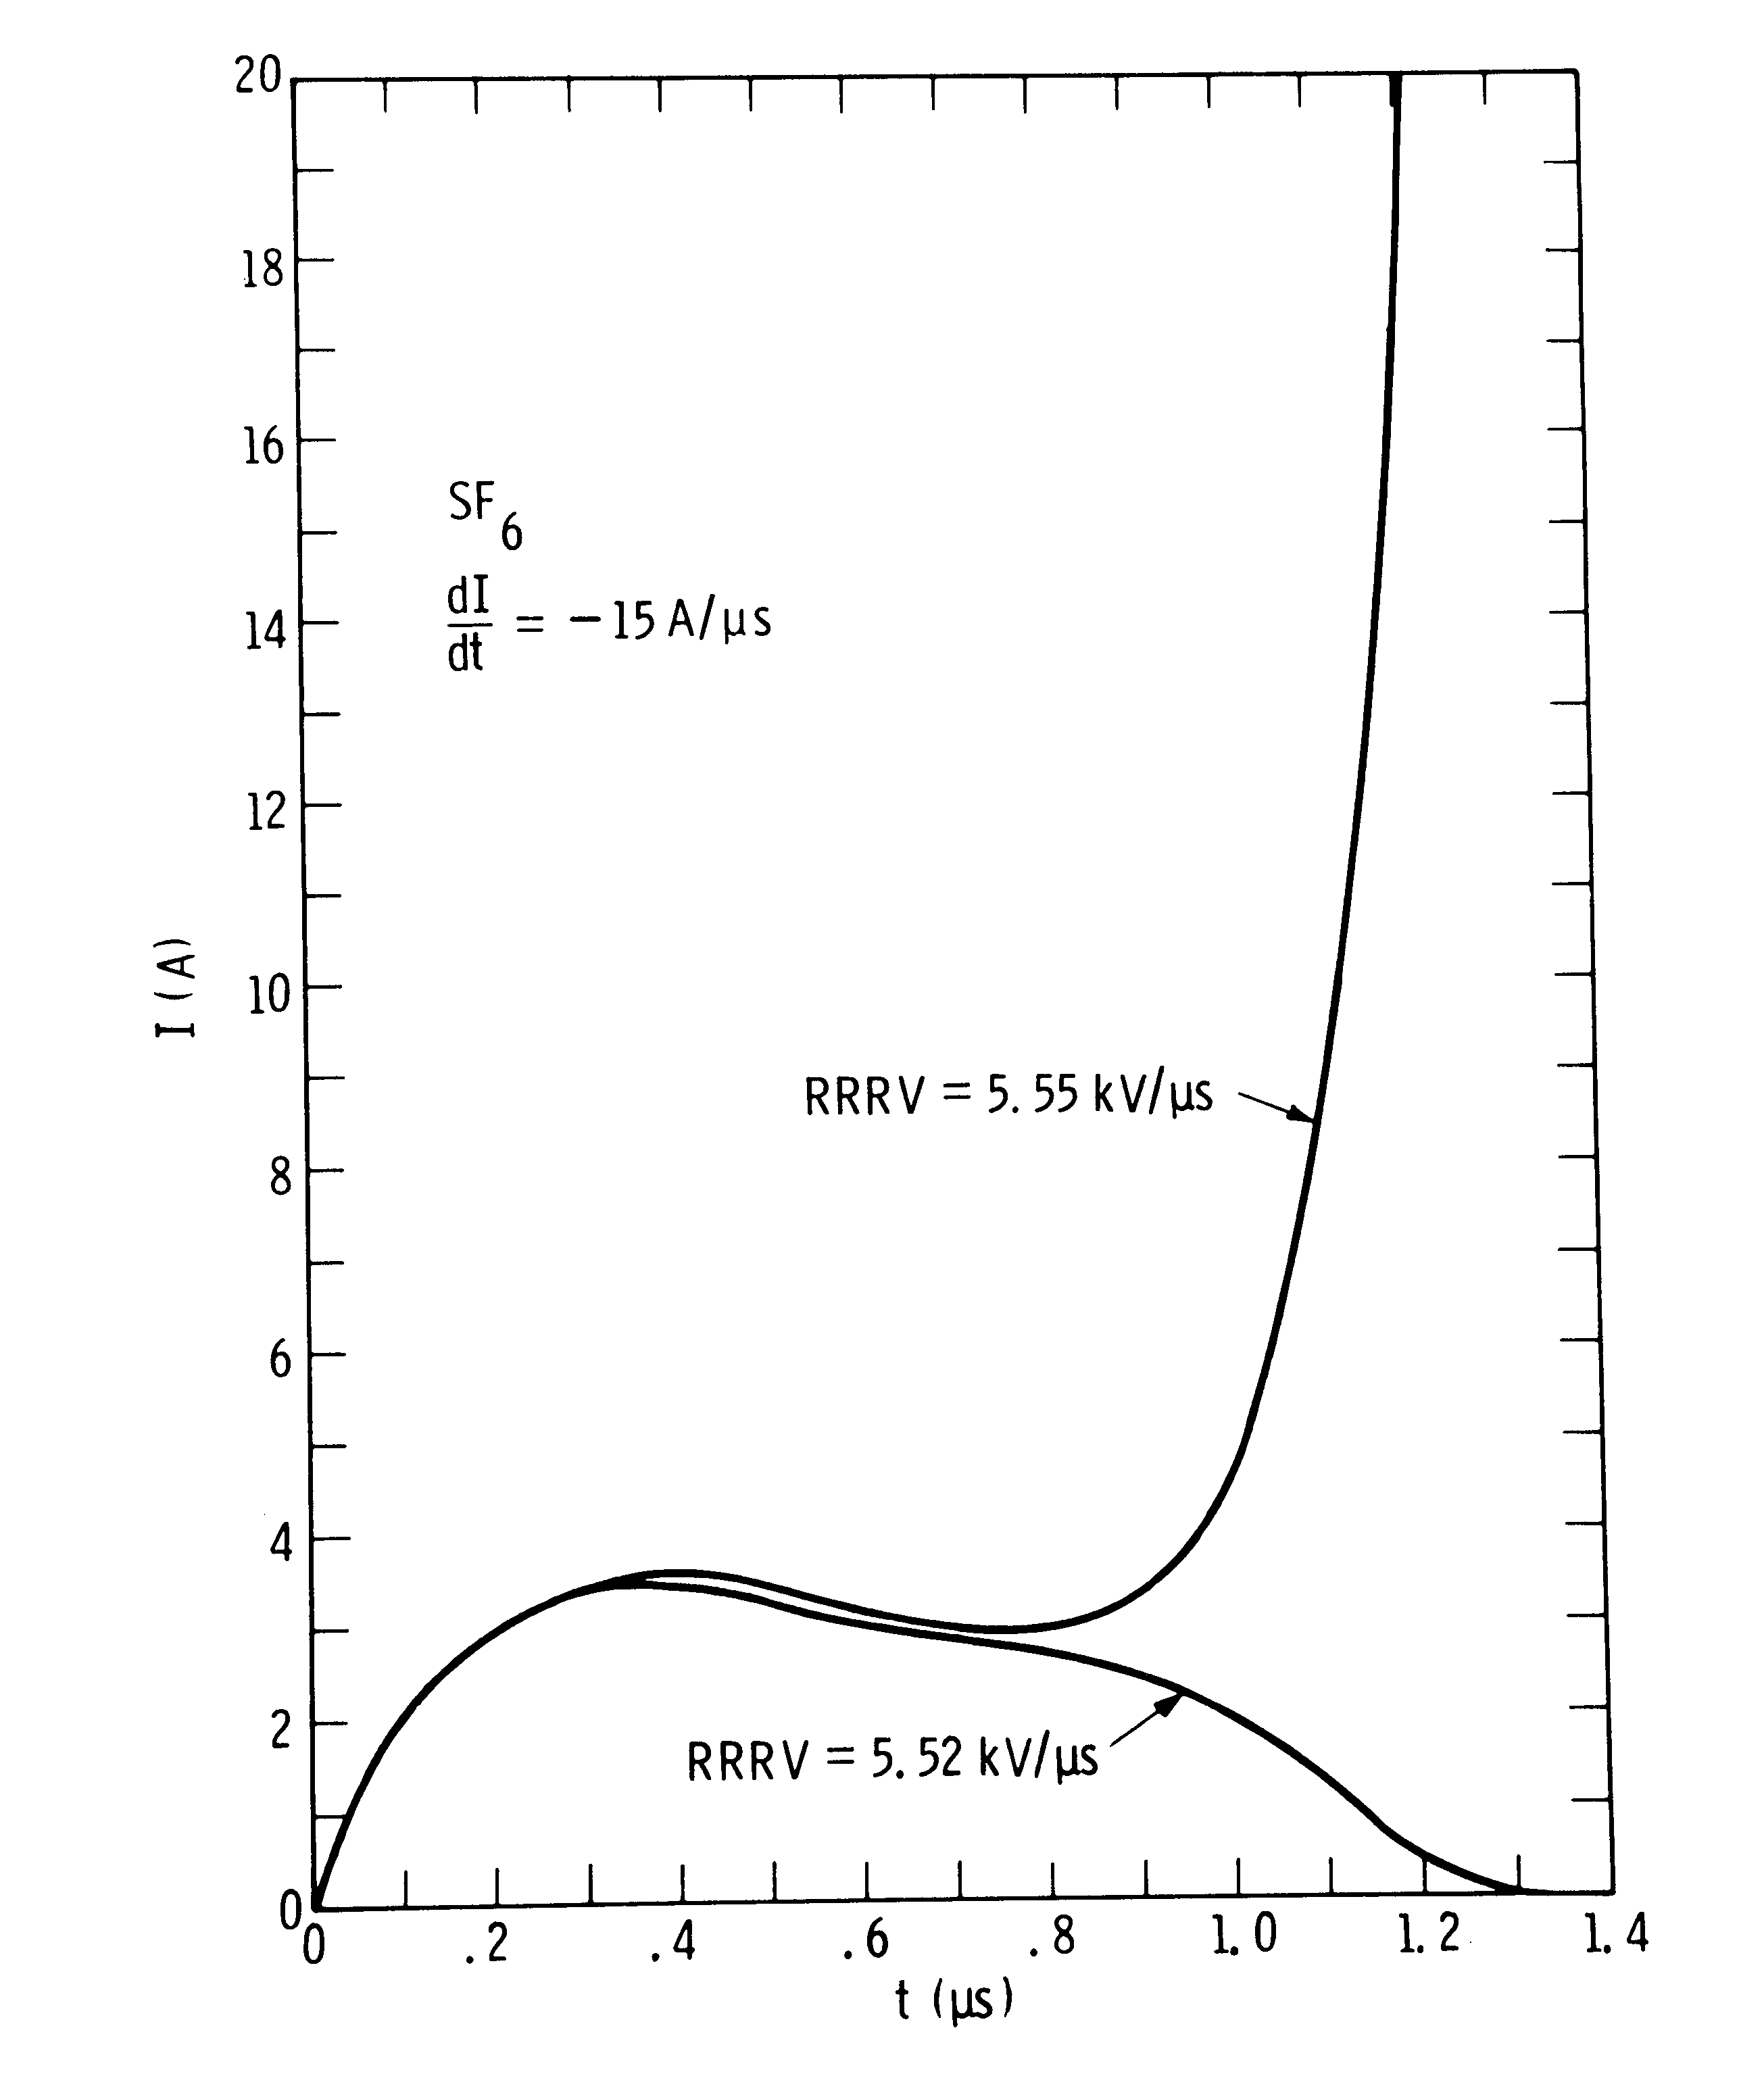
\includegraphics[scale=0.7]{Bilder/Theory/failSuccPAC.png}
\caption{The post-arc current during a successful and unsuccessful interruption \cite{bib:CIHVN}.} \label{fig:PACbreakandreIgnite}
\end{figure}

The thermal interruption success rate is partly determined by the amount of stored energy in the arc and in its surroundings. Power is the product of arcing voltage and current. The energy produced by the arc is the integral of the power during a certain time span. Research has shown that only the energy dissipated close to CZ has an effect on the interruption capabilities, and that the cooling from the air flow mainly effects the interruption rate between 50 to 100 microseconds before CZ \cite{bib:CIHVN}.

The parameter $d \mathrm{I}/d \mathrm{t}$ can be used to describe the energy losses close to CZ. In figure \ref{fig:freqComp}, two currents with the same $d \mathrm{I}/d \mathrm{t}$ close to CZ can be observed.

\begin{figure} [H]
\centering
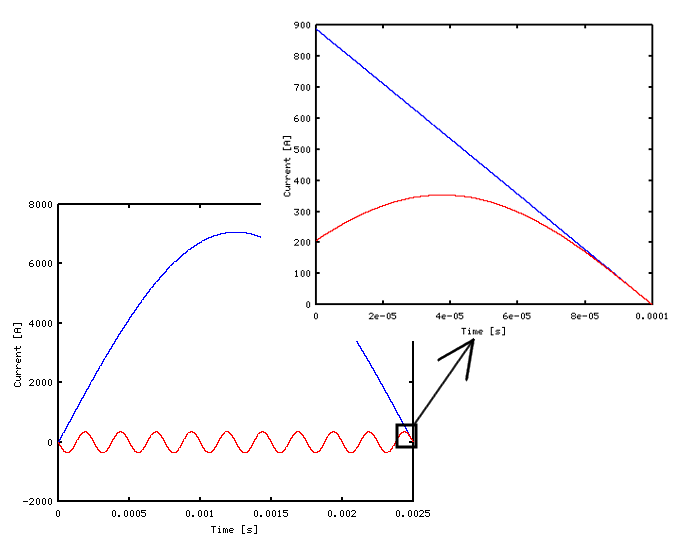
\includegraphics[scale=0.6]{Bilder/Theory/diffFreq3.png}
\caption{Comparison of $d \mathrm{I}/d \mathrm{t}$ for a 200 Hz and 4000 Hz current wave.} \label{fig:freqComp}
\end{figure}

These two currents, even though they have completely different frequency and amplitude, have proven almost equally difficult to interrupt \cite{bib:CIHVN}. Therefore, it is assumed that the effect of a puffer is most efficient close to CZ, where the energy dissipation is almost equal, and right after CZ, when the PAC is present. The graph in the lower part of the picture in figure \ref{fig:freqComp} shows a half period of the 200 Hz current next to several periods of the 4000 Hz current, while the upper part of the figure shows both currents 100 $\mu$s before CZ. As can be seen form the figure, $d \mathrm{I}/d \mathrm{t}$ for the 200 Hz and the 4000 Hz current are almost alike for the last 50 $\mu$s before CZ.

The thermal inertia of the interruption gas, as described with the time constants presented in table \ref{tab:timeConstants}, can give an idea of the rate the PAC is reduced. Gases with a long time constant will probably have a longer time span for the PAC. In air based LBSs, thermal re-ignitions are considered a huge challenge, and this problem may partially be explained by the long duration for the PAC.

As described in this section, the probability of thermal re-ignition can depend on several factors. The $d \mathrm{I}/d \mathrm{t}$ close to CZ will give an estimate of the energy dissipation in the arc and the temperature in the plasma. This will both influence the current peak and time of the PAC. The time constant of the interruption gas gives an indication of how fast the gas responds to changes from for example cooling. The effect of cooling on the arcing voltage and the energy dissipation close to CZ will be investigated in the following experimental work in this report. A long time constant might lead to slower cooling of the arc, resulting in a higher amplitude and time span of the PAC. The steepness of the recovery voltage is also important, as a fast increase in this voltage will accelerate the charge carriers that make up the PAC, resulting in a larger probability of re-ignition. Further information on this topic can be collected from the book "Current Interruption in High-Voltage Networks" \cite{bib:CIHVN}.


\subsection{Air flow considerations}
During the interruption process, a puffer based switch uses a piston to drive an air flow to quench the arc. The energy loss from the arc is transported away by this air flow as described in section \ref{sec:HeatTransport}. The efficiency of the cooling depends on the speed and mass of the air flow, as well as how the flow is guided onto the arc. In figure \ref{fig:airPressurePuffer2}, a typical pressure during interruption in the pressure chamber of an LBS is illustrated. However, in the test switch presented in section \ref{sec:testSwitchandContact} and used in the interruption tests conducted in this report, the pressure is more or less constant throughout the whole interruption process. This is because it uses a large pressure reservoir rather than a piston to drive the air flow.

The mass flow, $\dot{m}$, of air through the nozzle can in most interruption cases be regarded as conserved, and is presented in equation \eqref{eq:massFlow}. The mass density, $\rho$, depends on pressure and temperature, while the volume flow, \textit{Q}, depends on speed and area, as presented in equation \eqref{eq:volumeFlow}.

\begin{equation} \label{eq:massFlow}
\dot{m}=\rho Q
\end{equation} 

\begin{equation} \label{eq:volumeFlow}
Q=\int v \ dA
\end{equation}

In equation \eqref{eq:volumeFlow}, the area, \textit{A}, is the cross-section area of the nozzle if considering the volume flow rate in a nozzle. This will vary depending on where in the nozzle the volume flow is calculated, as well as the arcing contact's position. The speed of the air flow, $v$, depends on the pressure difference, $\Delta p$, between the pressure chamber and the interruption chamber, and it will increase with an increasing pressure difference. An increase in air flow velocity will result in a greater mass flow, which if guided properly will lead to a more efficient cooling of the arc. In the test switch used during the experiments conducted in this report, the efficiency of the cooling can be set by adjusting the pressure in the pressure reservoir before interruption as described in section \ref{sec:testCir}.

\cleardoublepage
\section{Method}

\subsection{Test circuit} \label{sec:testCir}

Figure \ref{fig:testSwitchRiggEq} illustrates the physical appearance of the test switch. The numbered parts are: 1. Compressed air reservoir (connected to the high voltage supply circuit), 2. Tulip contact, 3. Nozzle, 4. Pin contact, 5. Connection to load circuit, 6. Spring drive mechanism, 7. Electromagnet release mechanism, and 8. Position transducer.

\begin{figure} [H]
\centering
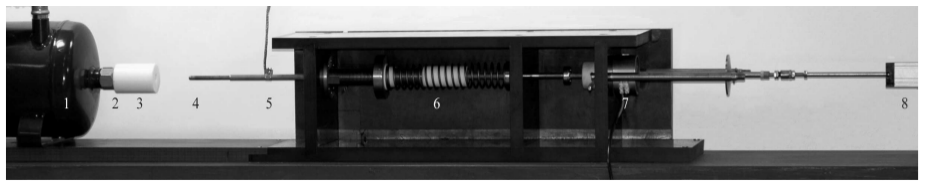
\includegraphics[scale=0.43]{Bilder/Method/switchTest.png}
\caption{The physical appearance of the test switch \cite{bib:AFIMVLBA}.} \label{fig:testSwitchRiggEq}
\end{figure}

Figure \ref{fig:testCurcuit} displays the laboratory test circuit used for the interruption tests. The circuit is designed to supply a current of 50 Hz / 13.8 kV. It is possible to shape the transient recovery voltage (TRV) by tuning the parameters L$_1$, L$_s$, R$_1$, R$_d$, and C. The systems' short circuit parameters are R$_{sc}$ and L$_{sc}$. The TRV generated during interruption is set to simulate the standard for a 24 kV / 630 A class from the International Electrotechnical Commission (IEC), which corresponds to:

\begin{itemize}
\item The initial part of the TRV has a rate of rise in recovery voltage (RRRV) of 71 - 74 V / $\mu$s.
	\begin{itemize}
		\item The voltage difference is measured over the first 20 $\mu$s after CZ.
	\end{itemize}
\item The first voltage peak is between 7.0 and 7.4 kV, with a rise time of approximately 96 $\mu$s.
\end{itemize}

\begin{figure} [H]
\centering
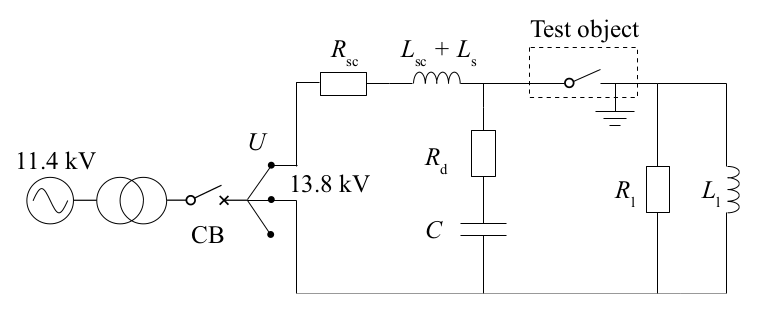
\includegraphics[scale=0.35]{Bilder/Method/circuit.png}
\caption{Circuit used for the interruption test \cite{bib:AFIMVLBA}.} \label{fig:testCurcuit}
\end{figure}

In table \ref{tab:testParameters}, the values of the different test circuit parameters and the corresponding currents can be observed. The test is conducted at currents with an RMS value of 630 A and 880 A. During the entire experiment, the TRV is kept constant up to and including the first voltage peak. In the case of a failed interruption, a thermal re-ignition occurs within a few microseconds after CZ.

\begin{table}[H]
\center
\caption{Circuit parameters and resulting currents \cite{bib:AFIMVLBA}. }
\begin{tabular}{|c|c|c|c|c|c|}
\hline 
L$_s$ [mH] & L$_1$ [mH] & R$_1$ [$\Omega$] & C [nF] & R$_{d}$ [$\Omega$] & I [A] \\ 
\hline 
6.9 & 86.2 & 22.1 & 102 & 198 & 630 \\ 
\hline
2.9 & 60.2 & 15.1 & 156 & 170 & 880 \\
\hline   
\end{tabular} 
\label{tab:testParameters}
\end{table}

A resistive transducer is measuring the contact position, while a Hall Effect current transducer is measuring the current through the test switch. The voltage between the contacts is measured with a parallel resistive / capacitive voltage divider. All measurements are transmitted through optical fibres to a 12 bit resolution transient recorder with a sampling frequency of 2.5 MHz. The pressure in the tank is only measured before each test, and with an accuracy of 0.01 bar. 

A near-infrared (NIR) high-speed camera produced by Xeneth called Cheetah 1470, records the opening sequence of the switch and the arc that burns between the contacts with a frame rate of approximately 10 000 fps, with an integration time of 3.7 $\mu$s and an image resolution of $384 \times 120$. The camera lens used is a 75 mm Apochromat Kiroptik Paris Nr. 99585, with an adjustable f-number set to f/16. %In appendix \ref{app:softwareSettings} the relevant software settings for the camera can be seen.??

\subsection{The switch and contact geometry} \label{sec:testSwitchandContact}
This experiment is conducted using copper-tungsten arcing contacts, polytetraflourelthylene (PTFE) nozzles, and air as interrupting medium. Copper-tungsten arcing contacts and a PTFE nozzle is commonly applied in commercial LBSs, and is therefore used in this experiment. PTFE is also chemically stable during the arcing time, which prohibits vaporisation products from the nozzle to influence the interruption capabilities of the test switch. As mentioned in section \ref{sec:InterruptCurrent}, copper-tungsten is applied because it is highly resistant from stresses from the arc. The system is an open system, with the surrounding air at atmospheric pressure, \textit{p$_0$}, and a six-litre tank with a pre-filled upstream overpressure, \textit{p$_u$}, used during the interruption process to quench the arc. It is possible to adjust the upstream pressure, contact speed, and position at current zero (CZ) independently, as well as the contact and nozzle geometry. The current and TRV can be manipulated by changing the parameters of the laboratory test circuit, as described in section \ref{sec:testCir}.

Two different kinds of nozzle designs are going to be tested. One of the nozzle designs has a short nozzle with a funnel shape at the end. It consists of two different contact geometries, which are denoted \textbf{a} and \textbf{b}. The other nozzle design has a longer nozzle with a cylindrical shape, this contact geometry is denoted \textbf{c}. 

The contact position \textit{x} is defined as the axial distance between the tulip and the pin contact. At starting position, \textit{x}= -60 mm, the pin contact is acting as a plug for the tank. This makes it possible to pre-set an upstream over-pressure. The contact is held in place by an electromagnet, and is set to motion when the magnet releases a compressed spring. The spring accelerates the pin contact up to a speed of approximately 5.5 m/s at \textit{x}=0. At this position, the spring is unloaded and the pin moves with a constant speed until the contact is fully open at \textit{x}=110 mm.

A simple drawing of the contact and nozzle for geometry \textbf{a} and \textbf{b} is displayed in figure \ref{fig:contactAndNozzle}. The length of the nozzle is 20 mm, and its inner diameter is \textit{D}. Axial symmetry is present along the x-axis. The dimensions of geometry \textbf{a} and \textbf{b} are given in table \ref{tab:contGeoPara}, and the definitions of the different areas are illustrated in figure \ref{fig:AreacontactAndNozzle}. Previously conducted experiments presented in the paper "Air flow investigation for a medium voltage load break switch" \cite{bib:AFIMVLBA} have suggested that the interruption success rate is better outside the nozzle than inside the nozzle. During a normal interruption, when a switch is applied in the transmission grid, the position of the pin at the moment of CZ is random. Therefore, a short nozzle is used, since this will (in an interruption outside the laboratory) increase the probability for the first CZ to occur outside the nozzle. Due to the difference in interruption rate between inside and outside of the nozzle, a funnel shape at the end of the nozzle is applied. This results in a smoother transaction between the inside and the outside, so that the sudden change in interruption rate can be better analysed. The funnel shape also makes it more alike a commercial nozzle design.


\begin{figure} [h]
\centering
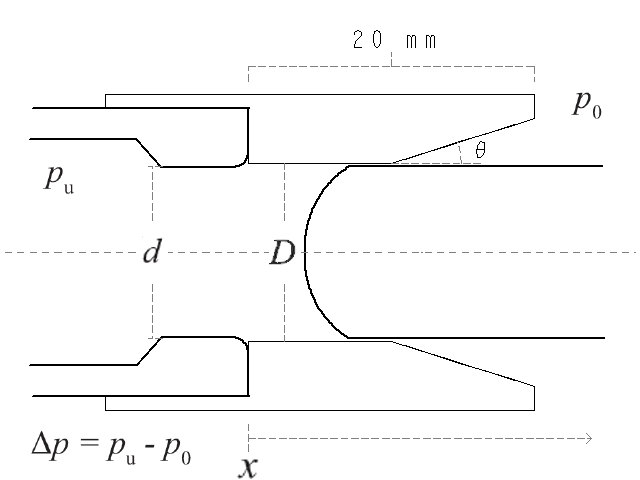
\includegraphics[scale=0.45]{Bilder/Method/ContactAndNozzleFunnelShape5.png}
\caption{Diagram over the contact and nozzle for geometry \textit{a} and \textit{b}. The diameter of the contact is \textit{d}, and the inner diameter of the nozzle is \textit{D}. In table \ref{tab:contGeoPara}, the differences between the two geometries are shown.} \label{fig:contactAndNozzle}
\end{figure}

\begin{figure} [H] %denne må byttes ut.
\centering
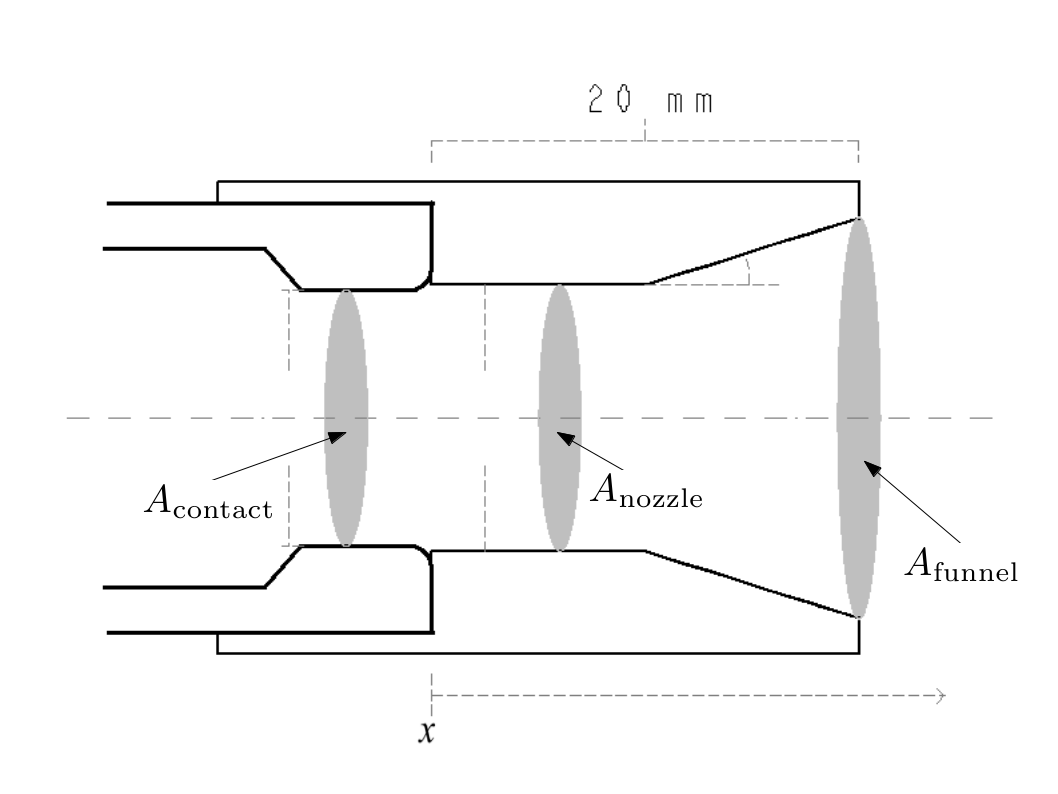
\includegraphics[scale=0.30]{Bilder/Method/AreaDef.png}
\caption{Overview of the definitions of the areas.} \label{fig:AreacontactAndNozzle}
\end{figure}

For geometry \textbf{a} and \textbf{b} the following definitions apply:
\begin{itemize}
\item $A_\mathrm{{contact}}$ is the cross section of the contact pin, as well as the area of the tulip contact. The area is described by equation \eqref{eq:A_contact}.

\item $A_\mathrm{{nozzle}}$ is defined as the area of the cylindrical part of the nozzle, where x=[0,10] mm. The area is described by equation \eqref{eq:A_nozzle}.

\item $A_\mathrm{{funnel}}$ is defined as the area at the end of the nozzle, where x=20 mm, and the diameter of the funnel is at its largest. This area is described by equation \eqref{eq:A_funnel}.

\item The angle $\mathrm{\theta}$ is defined so that $A_\mathrm{{funnel}}=4 \cdot A_\mathrm{{nozzle}}$ for each geometry.

\item $A_\mathrm{{ring}}$ is in table \ref{tab:contGeoPara} defined as the area between the pin contact and the cylindrical part of the nozzle, where x=[0,10] mm, and is described by equation \eqref{eq:A_ring_1}. For x=[10,20] mm, $A_\mathrm{{ring}}$ is a function of the pin's position, x, inside the nozzle, described by equation \eqref{eq:A_ring_2}.
\end{itemize}

\begin{equation} \label{eq:A_contact}
A_\mathrm{{contact}}=A_\mathrm{{tulip}}=\pi \frac{d^2}{4}
\end{equation}
\begin{equation} \label{eq:A_nozzle}
A_\mathrm{{nozzle}}=\pi \frac{D^2}{4}
\end{equation}

\begin{equation} \label{eq:A_funnel}
A_\mathrm{{funnel}}=4 \cdot A_\mathrm{{nozzle}}=4\pi \frac{D^2}{4}
\end{equation}

\begin{equation} \label{eq:A_ring_1}
A_\mathrm{{ring}}=A_\mathrm{{nozzle}}-A_\mathrm{{contact}}=\pi\left( \frac{D^2}{4}-\frac{d^2}{4}\right)
\end{equation}
\begin{equation} \label{eq:A_ring_2}
A_\mathrm{{ring}}(x)=\pi\left( \left(\frac{2(x-10)\tan \theta + D}{2}\right)^2-\frac{d^2}{4}\right)
\end{equation}

\begin{table}[H]
\center
\caption{Contact geometry parameters for the funnel shaped nozzle design.}
 \begin{tabular}{|c|c|c|c|c|c|c|c|c|}
\hline 
Geometry & \textit{D} & \textit{d}  & $\frac{D}{d}$ & $\mathrm{\theta}$ & $A_\mathrm{{contact}}$ & $A_\mathrm{{ring}}$  & $A_\mathrm{{nozzle}}$ & $A_\mathrm{{funnel}}$ \\
  & [mm] &  [mm] &   &   &   [mm$^2$] &  [mm$^2$] &   [mm$^2$] &   [mm$^2$]\\
\hline 
\textbf{a} & 6.25 & 6.0 & 1.04 & 17.4 & 28.3 & 2.4 & 30.7 & 122.8\\ 
\hline 
\textbf{b} & 7.40 & 7.1 & 1.04 & 20.3 & 39.6 & 3.4 & 43.0 & 172.0\\ 
\hline 
\end{tabular} 
\label{tab:contGeoPara}
\end{table}

In figure \ref{fig:contactAndNozzleC}, the contact geometry denoted \textbf{c} is presented. The length of the nozzle is 30 mm, and axial symmetry is present along the x-axis. The diameter of the contact is \textit{d}, and the inner nozzle diameter is \textit{D}. The dimensions for the geometry is given in table \ref{tab:contGeoParaC}. $A_\mathrm{{contact}}$ and $A_\mathrm{{nozzle}}$ are defined in the same way as for geometry \textbf{a} and \textbf{b}, as presented in equation \eqref{eq:A_contact} and \eqref{eq:A_nozzle}. The nozzle is cylindrical for its entire length (x=[0,30] mm), therefore, $A_\mathrm{{funnel}}$ does not exist for this geometry and $A_\mathrm{{ring}}$ is defined as in equation \eqref{eq:A_ring_1} for the entire length of the nozzle, x=[0,30] mm. 

As stated in section \ref{sec:puffer}, a LBS design is often a scaled down version of a circuit breaker design. A result of this is that a common contact diameter is approximately 11 mm. However, test results presented in the paper: "Air flow investigation for a medium voltage load break switch" \cite{bib:AFIMVLBA} have suggested that the optimal contact diameter depends on the current passing through the switch. In the paper mentioned above, tests for another geometry (denoted \textbf{d} in this report), which has the same D/d as geometry \textbf{c}, has been conducted, and results from this test are going to be compared with the interruption test results for geometry \textbf{c}. Geometry \textbf{d} has a \textit{d}=6.0 mm, which seems to be the optimal value for a current of 630 A. From the previously conducted test results on geometry \textbf{d}, Nina Sasaki Aanensen has calculated that the optimal contact diameter for a current of 880 A is 7.1 mm. Therefore, this value has been selected as contact diameter for geometry \textbf{c}. Contact geometry parameters for geometry \textbf{c} and \textbf{d} are presented in table \ref{tab:contGeoParaC}.

\begin{figure} [H]
\centering
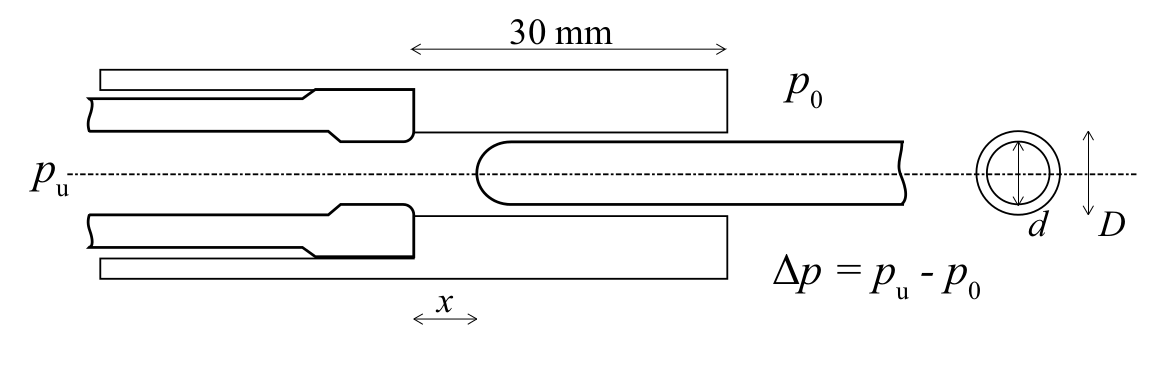
\includegraphics[scale=0.3]{Bilder/Method/contactSetUp.png}
\caption{Diagram over the contact and nozzle for geometry \textit{c} and \textit{d}. The diameter of the contact is \textit{d}, and the inner diameter of the nozzle is \textit{D}. In table \ref{tab:contGeoParaC}, the differences between the two geometries are shown \cite{bib:AFIMVLBA}.} \label{fig:contactAndNozzleC}
\end{figure}

\begin{table}[H]
\center
\caption{Contact geometry parameters for the cylindrical shaped nozzle design.}
 \begin{tabular}{|c|c|c|c|c|c|c|}
\hline 
Geometry & \textit{D} & \textit{d}  & $\frac{D}{d}$ &  $A_\mathrm{{contact}}$ & $A_\mathrm{{ring}}$  & $A_\mathrm{{nozzle}}$ \\
  & [mm] &  [mm] &   &  [mm$^2$] &  [mm$^2$] &   [mm$^2$] \\
\hline 
\textbf{c} & 9.6 & 7.1 & 1.35 & 39.6 & 32.8 & 72.4 \\ 
\hline
\textbf{d} & 8.0 & 6.0 & 1.33 & 28.3 & 22.0 & 50.3 \\ 
\hline
\end{tabular} 
\label{tab:contGeoParaC}
\end{table}

\subsection{Procedure} \label{sec:procedure}
Interruption tests with CZ occurring both inside and outside of the nozzle are carried out. Six types of tests in total are conducted in this interruption experiment. One type of test consists of one contact geometry at a current magnitude of either 630 A or 880 A with a minimum of:
\begin{itemize}
\item For geometry \textbf{a} and \textbf{b}: \\
Five interruptions inside of the funnel part of the nozzle and five interruptions outside of the nozzle at each pressure level.

\item For geometry \textbf{c}: \\
Five interruptions outside of the nozzle at each pressure level.

\end{itemize}
At least three different pressure levels are included in each test. Both the first and second CZ are included in this study in order to provide as much data as possible.

For geometry \textbf{a} and \textbf{b} "inside funnel" is defined as contact position x = [11, 19] mm and "outside nozzle" as x = [21, 60] mm for the first CZ. A boundary region of 1 mm is added between the end of the cylindrical part of the nozzle and the start of the funnel part of the nozzle, and a similar boundary region of 2 mm is added between the end of the funnel part of the nozzle and outside of the nozzle. Results that occurs in this boundary region are discarded in order to be certain of which region the CZ occurred in. Results from zero crossings that occurs in the cylindrical part of the nozzle, x $<$ 10 mm, between the tulip contact and the start of the funnel-shaped nozzle are discarded. For geometry \textbf{c} "outside nozzle" is defined as x = [35, 60] mm at first CZ. Interruptions that occurs "inside nozzle", x $<$ 30 mm, or in the boundary region between inside and outside the nozzle, x = [30, 35] mm, for geometry \textbf{c} are discarded. The first CZ occurs within x $<$ 60 mm, and the second CZ occurs for x $>$ 60 mm, as the contact speed during all tests is 5.5 mm/ms $\pm$ 0.5 mm/ms. When testing the interrupting capabilities inside the funnel, the first CZ is aimed to occur at x=15 mm. When testing outside the nozzle, the first CZ is aimed at x=30 mm for geometry \textbf{a} and \textbf{b}, and x=45 mm for geometry \textbf{c}. Due to variation in the travelling speed of the contacts and activation time of the release mechanism, some difference in the position of the pin at the moment of CZ will occur between each interruption attempt.

When testing the interrupting capabilities, the test procedure for each of the six cases is as follows: 

\begin{itemize}
\item[1.] A pressure level that seems to be in the area of interest is found by performing some initial test interruptions at different pressure levels. This level is kept constant for at least five interruption tests.
\item[2.] If a pressure level results in less than 100\% successful interruptions, at least five new tests with a higher upstream pressure (next level) are conducted. This is repeated until at least one pressure level with five successful interruptions is found.
\item[3.] Then, the pressure is stepped down until 60\% or more of the interruption attempts fail, or the lowest possible pressure level is tested.
\end{itemize}

When testing for variations in the arcing voltage between a successful and an unsuccessful interruption, a pressure level where the interruption success rate is 50\% is used. Then, five successful interruptions and five unsuccessful interruptions are obtained while the arcing voltage is measured and stored for further use. All the interruptions should take place so that the second CZ occurs at x=75 mm. The switching process is filmed by a NIR high-speed camera so that the path of the arc can be monitored during the interruption.

The pin is cleaned, polished, and greased between each test to ensure a smooth surface. The contact members and nozzle are replaced regularly to avoid contact wear and nozzle deformation. This is to ensure that the geometry has a constant form through the whole experiment.
\cleardoublepage

\section{Results and Discussion}
\subsection{Interruption tests} \label{sec:interruptionTests}
\subsubsection{Interpretation and differentiation of interruption results}
In the following section interruption results from the tests conducted on all the three geometries are presented. For each interruption test there are two final results: success or failure. The final result is determined by the interruption outcome from the first or second CZ. At the first CZ the interruption can succeed or a re-ignition can occur. A re-ignition can be either thermal or dielectric. Given a re-ignition in the first CZ, the current can be interrupted at the second CZ, or another re-ignition can occur. The outcomes are explained by figure \ref{fig:flowchart}. The total interruption success rate for a geometry at a pressure level, is based on the "final result" for a given number of interruption tests at that pressure level. The number of interruption tests at each pressure level depends on which geometry that are being tested as described in section \ref{sec:procedure}. 

\begin{figure} [H]
\centering
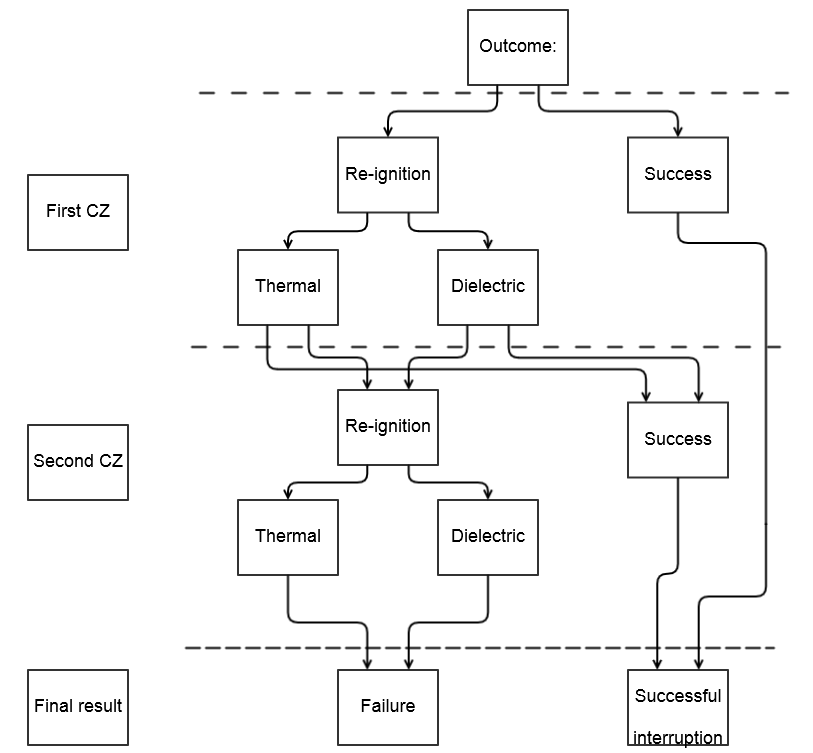
\includegraphics[scale=0.6]{Bilder/Results/outcomeinterruption.png}
\caption{Flowchart over different interruption outcomes.} \label{fig:flowchart}
\end{figure}

Previously conducted tests have shown that the most common re-ignition is a thermal re-ignition, and experience has also indicated that in practical interruption cases thermal re-ignitions are the most demanding tasks for load break switches in the 24 kV/630 A class \cite{bib:AFIMVLBA}. However, dielectric re-ignitions can also occur usually at the first CZ.

In figure \ref{fig:CurrentAndVoltageWaveform}, the current and voltage during an unsuccessful and a successful interruption are shown for a 630 A/24 kV test. The upper plot illustrates a thermal re-ignition, as the plot illustrates; the current is almost unaffected of the interruption attempt and continues as normal after the CZ. The lower plot is illustrating a successful interruption, where the current has stopped flowing after CZ and a TRV has risen between the contact members. 

In figure \ref{fig:CurrentAndVoltageDRWaveform}, the voltage and current during a dielectric re-ignition are shown for an 880 A/24 kV test. As can be seen from the figure, the current stops flowing for more than one millisecond after the CZ before the electrical field caused by the TRV, which has risen between the contact members, becomes too strong and results in an electrical breakdown of the air. Then the current continues to flow and will quickly obtain the sinusoidal form set by the supply side of the switch. 

\begin{figure}[H]
\centering
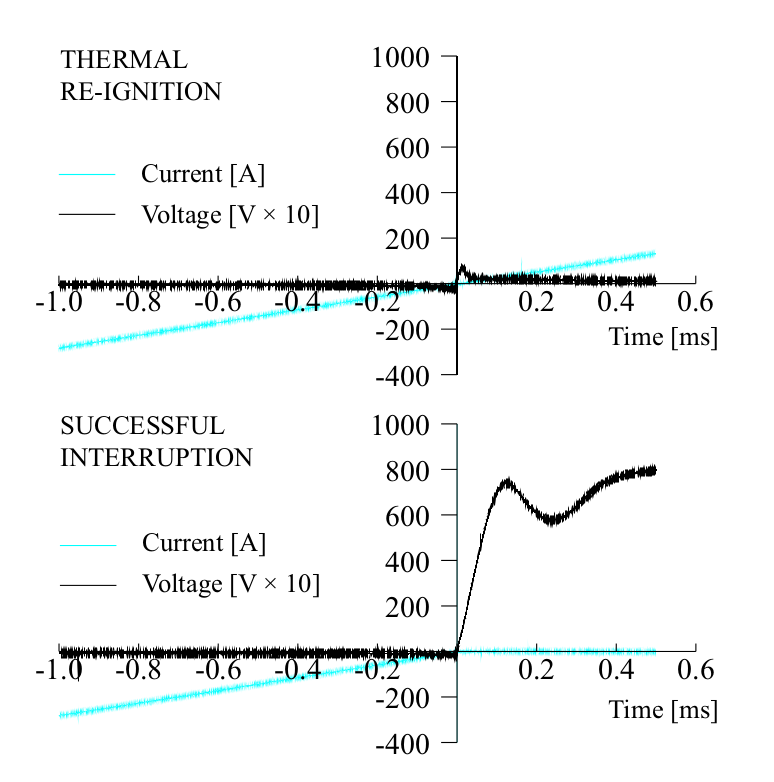
\includegraphics[scale=0.32]{Bilder/Results/differentInterruptions.png}
\caption{Current and voltage waveforms near CZ for a thermal re-ignition and a successful interruption \cite{bib:AFIMVLBA}.} \label{fig:CurrentAndVoltageWaveform}
\end{figure}

\begin{figure}[H]
\centering
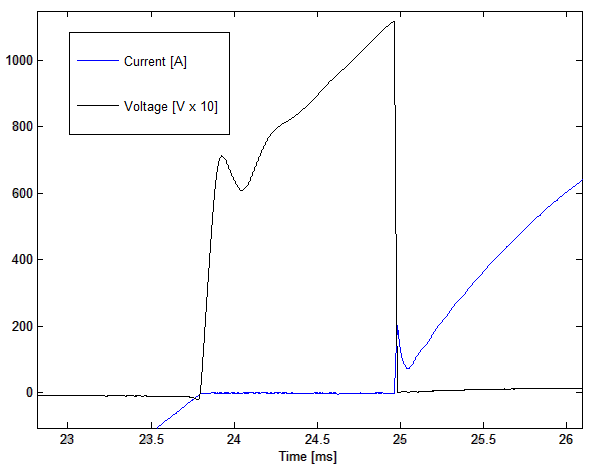
\includegraphics[scale=0.7]{Bilder/Results/DRplot2.PNG}
\caption{Current and voltage waveforms near CZ for a dielectric re-ignition.} \label{fig:CurrentAndVoltageDRWaveform}
\end{figure}

\subsubsection{Interruption results for geometry \textbf{a}}

\subsubsection*{630 A interruption tests}

In figure \ref{fig:results630AgeoA}, the total interruption success rate for the 630 A test for geometry \textbf{a} is presented. Each data point consists of 10 tests. For five of the tests, the first CZ occurred inside the funnel part of the nozzle, while the remaining five tests occurred outside of the nozzle. Key values for the total interruption success rate are presented in table \ref{tab:compgeoAandB} in section \ref{sec:compAandB}.

%As seen from figure \ref{fig:results630AgeoA} the 100\% interruption success rate occurred at an upstream over-pressure of 0.3 bar, while none successful interruptions where obtained at 0.15 bar upstream over-pressure. The 50\% interruption success rate can be obtained from the figure, and corresponds to an over-pressure of approximately 0.19 bar.

The results when comparing the interruption success rate between tests that occurred inside the funnel and outside the nozzle for the first CZ are presented in figure \ref{fig:results630AgeoAcomp}. In this figure each data point consists of five tests which occurred either "inside funnel" (purple line) or "outside nozzle" (red line). Both tests series have the same 100\% interruption success rate at an over-pressure of 0.3 bar and a 0\% interruption success rate at 0.15 bar over-pressure. The 50\% interruption success rate for the two series corresponds to approximately 0.18 bar over-pressure for "outside nozzle" and 0.22 bar over-presser for "inside funnel". In total the interruption success rate between "inside funnel" and "outside nozzle" is almost equal, even though, there is a difference between the 50\% interruption rates of the two series. Variance like this must be expected when each data point only consists of five tests.

\begin{figure}[H]
\centering
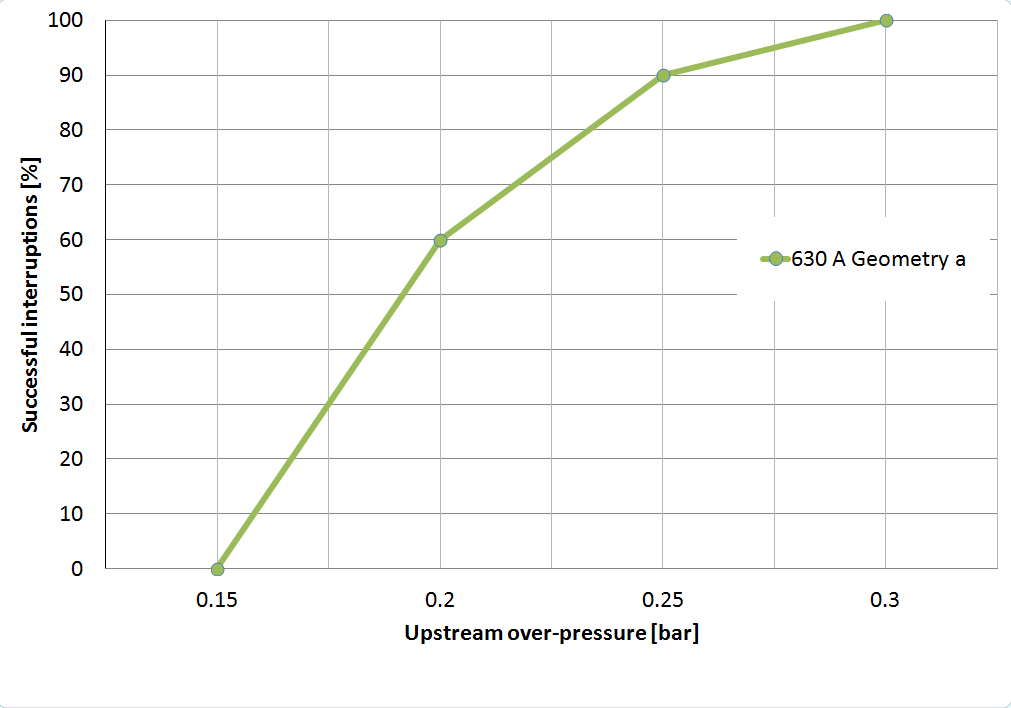
\includegraphics[scale=0.45]{Bilder/Results/geoA630amp_riktig.PNG}
\caption{Interruption test results for geometry \textbf{a} at 630 A when tests occurring "inside funnel" and "outside nozzle", and the results from the first and second CZ is added together.} \label{fig:results630AgeoA}
\end{figure}

\begin{figure}[H]
\centering
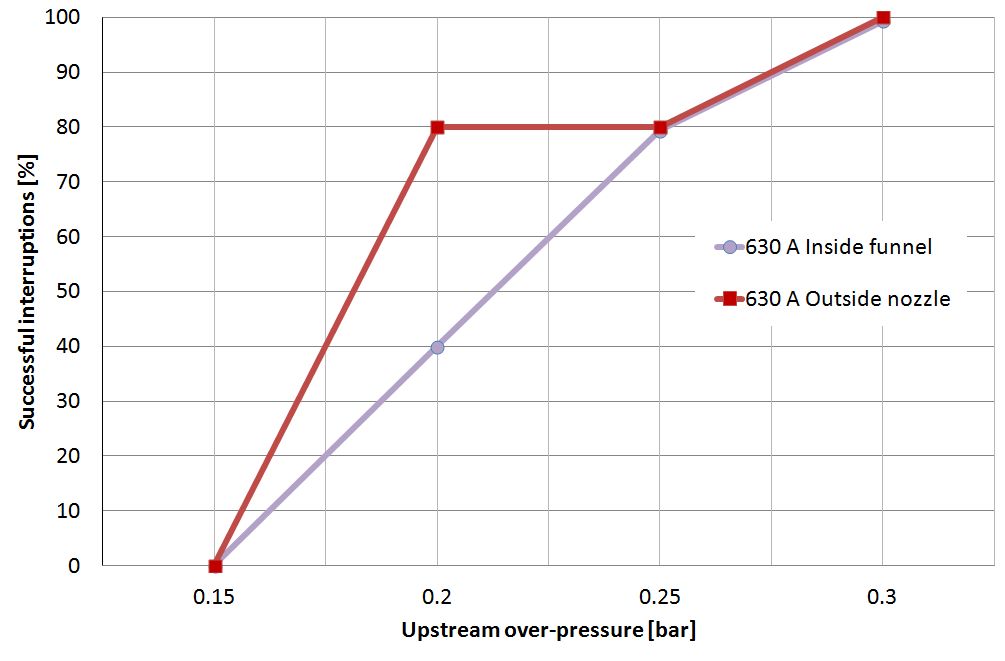
\includegraphics[scale=0.45]{Bilder/Results/geoA630ampcomp.PNG}
\caption{Interruption test results for geometry \textbf{a} at 630 A when only the first CZ is included and tests that occurred inside the funnel is separated from tests that occurred outside the nozzle.} \label{fig:results630AgeoAcomp}
\end{figure}

\subsubsection*{880 A interruption tests}
Due to wear of the nozzle when testing at 630 A for geometry \textbf{a} some alterations of the test procedure presented in section \ref{sec:procedure} were done for the 880 A test for geometry \textbf{a} to prevent running out of replacement nozzles. Instead of using five tests from "inside funnel" and five tests from "outside nozzle" for each data point in the 880 A interruption test, ten test with any x position were used as long as the first CZ occurred in the region where the pin's position was between 11 mm and 60 mm away from the tulip contact. From the interruption results presented for geometry \textbf{a} at 630 A and geometry \textbf{b} at 630 A and 880 A it can be seen that this simplification of the test procedure probably did not have a significant impact on the total interruption success rate, since the interruption success rate between "inside funnel" and "outside nozzle" are almost equal for all the other three conducted interruption cases for the funnel shaped nozzle designs. This reduced the total number of conducted tests, since many extra tests was performed in order to hit the desired region of the nozzle at the interruption tests for geometry \textbf{a} at 630 A, and geometry \textbf{b} at 630 A and 880 A. With the simplified test procedure the total interruption success rate where obtained and can be seen in figure \ref{fig:results880AgeoA}, and key values from it are presented in table \ref{tab:compgeoAandB} in section \ref{sec:compAandB}.


\begin{figure}[H]
\centering
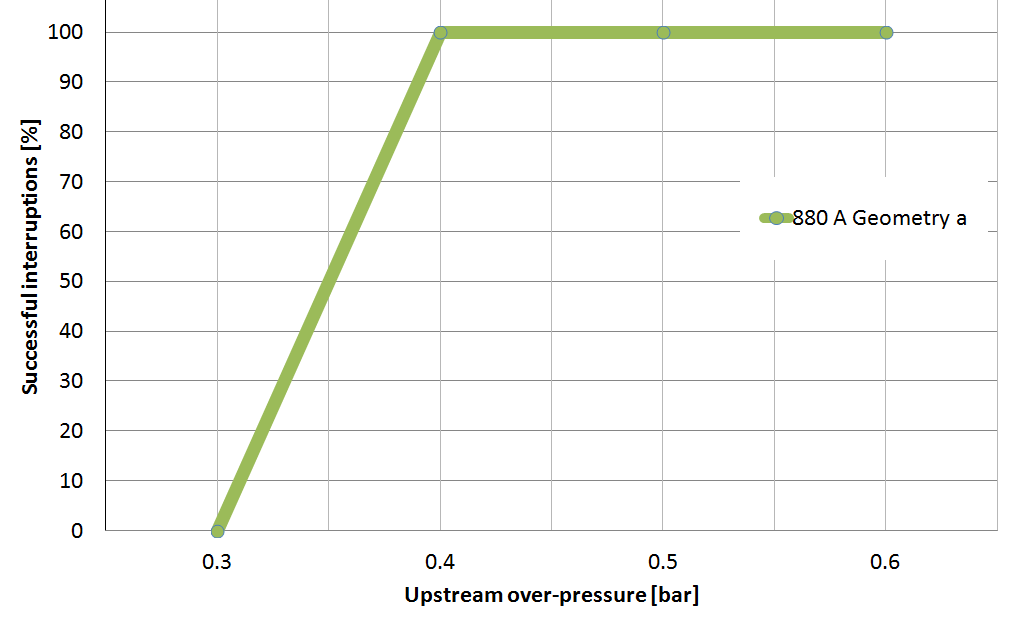
\includegraphics[scale=0.45]{Bilder/Results/geoA880Anew.PNG}
\caption{Interruption test results for geometry \textbf{a} at 880 A when tests occurring "inside funnel" and "outside nozzle", and the results from the first and second CZ is added together.} \label{fig:results880AgeoA}
\end{figure}

\subsubsection{Interruption results for geometry \textbf{b}} \label{sec:intTestGeoB}

\subsubsection*{630 A interruption tests}

In figure \ref{fig:results630AgeoB}, the total interruption success rate for the 630 A test for geometry \textbf{b} is presented. Each data point consists of 10 tests. For five of the tests, the first CZ occurred inside the funnel part of the nozzle, while the remaining five tests occurred outside of the nozzle. The lowest tested over-pressure was 0.15 bar with an interruption success rate of 10\%, more key values for the total interruption success rate are presented in table \ref{tab:compgeoAandB} in section \ref{sec:compAandB}. 

%As seen from figure \ref{fig:results630AgeoB} the 100\% interruption success rate occurred at an upstream over-pressure of 0.30 bar, while 10\% of the interruptions where successful at 0.15 bar upstream over-pressure, which were the lowest tested pressure. The 50\% interruption success rate can be obtained from the figure, and corresponds to an over-pressure of 0.175 bar.

The results when comparing the interruption success rate between tests that occurred inside the funnel and outside the nozzle for the first CZ is presented in figure \ref{fig:results630AgeoBcomp}. In this figure each data point consists of five tests which occurred either "inside funnel" (purple line) or "outside nozzle" (red line). The "outside nozzle" interruption test has a 100\% interruption success rate at an over-pressure of 0.25 bar and a 20\% interruption success rate at 0.15 bar over-pressure, which was the lowest pressure level tested. The test results for "inside funnel" experienced one re-ignition at the first CZ for 0.2 bar, 0.25 bar and 0.3 bar over-pressure, resulting in a 80\% interruption success rate for all these three pressure levels. However, it should be noted that the current was successfully interrupted at the second CZ at 0.3 bar and 0.2 bar upstream over-pressure when the pin was inside of the funnel at the first CZ. Therefore, the interruption success rate between the "inside funnel" and "outside nozzle" is almost equal if both CZs are taken into account. At the lowest tested pressure of 0.15 bar over-pressure, none successful interruptions where obtained. The 50\% interruption success rate for the two series were almost the same, and corresponds to an estimated value of 0.175 bar over-pressure "outside nozzle" and 0.18 bar over-pressure for "inside funnel". 


\begin{figure}[H]
\centering
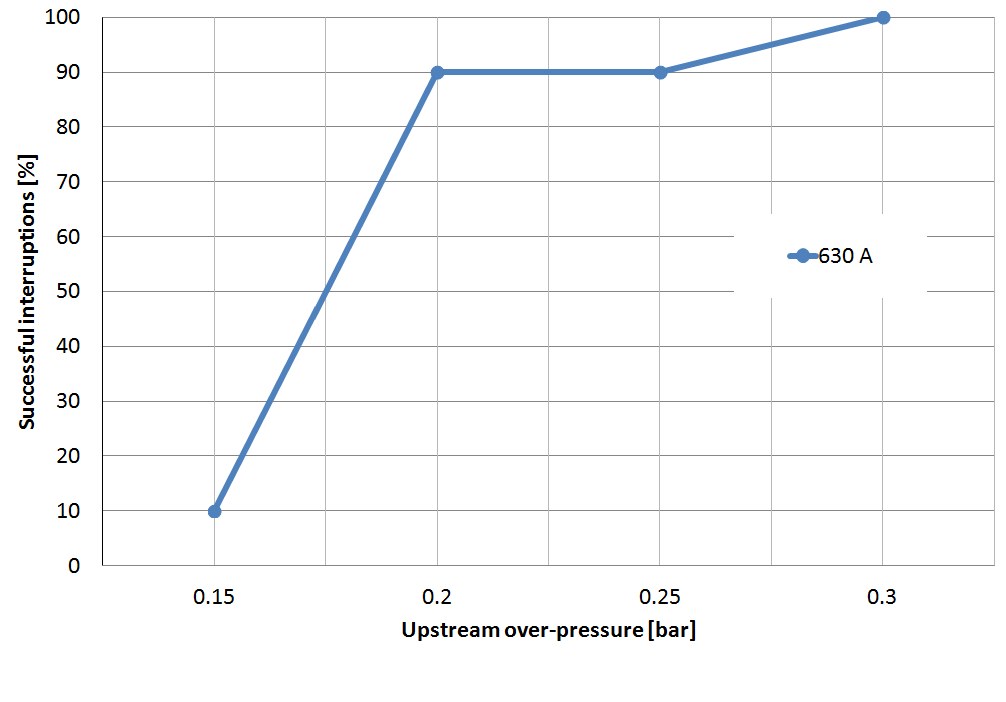
\includegraphics[scale=0.45]{Bilder/Results/geoB630amp.PNG}
\caption{Interruption test results for geometry \textbf{b} at 630 A when tests occurring "inside funnel" and "outside nozzle", and the results from the first and second CZ is added together.} \label{fig:results630AgeoB}
\end{figure}

\begin{figure}[H]
\centering
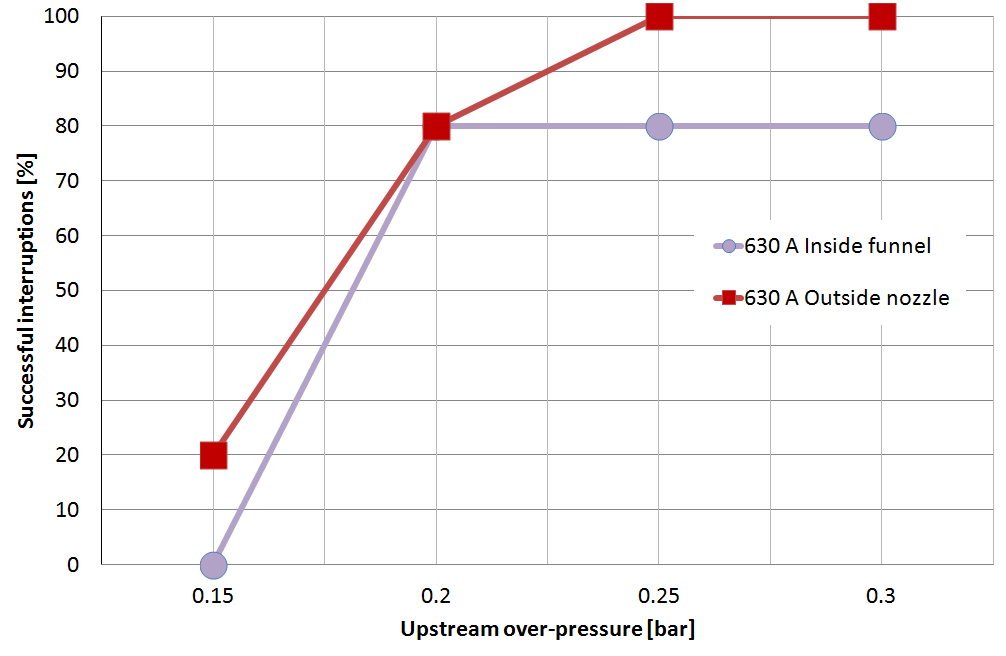
\includegraphics[scale=0.45]{Bilder/Results/geoB630ampcomp.PNG}
\caption{Interruption test results for geometry \textbf{b} at 630 A when only the first CZ is included and tests that occurred inside of the funnel is separated from tests that occurred outside of the nozzle.} \label{fig:results630AgeoBcomp}
\end{figure}

\subsubsection*{880 A interruption tests}

In figure \ref{fig:results880AgeoB}, the total interruption success rate for the 880 A interruption test for geometry \textbf{b} is presented. Each data point consists of 10 tests. For five of the tests, the first CZ occurred inside the funnel part of the nozzle, while the remaining five tests occurred outside the nozzle. Key values for the total interruption success rate are presented in table \ref{tab:compgeoAandB} in section \ref{sec:compAandB}. 

%As seen from figure \ref{fig:results880AgeoB} the 100\% interruption success rate occurred at an upstream over-pressure of 0.4 bar, while none successful interruptions where obtained at 0.25 bar upstream over-pressure. The 50\% interruption success rate can be obtained from the figure, and corresponds to an over-pressure of approximately 0.28 bar.

A compraison between the results from the interruption success rate between tests that occurred inside the funnel and outside of the nozzle for the first CZ is presented in figure \ref{fig:results880AgeoBcomp}. In this figure each data point consists of five tests which occurred either "inside funnel" (purple line) or "outside nozzle" (red line). The 100\% interruption success rate for tests inside the nozzle is at 0.4 bar over-pressure, while the 100\% interruption success rate for tests outside the nozzle is at 0.3 bar over-pressure. However, the "outside nozzle" test failed two times at higher pressures for the first CZ. One time at 0.35 bar and one time at 0.4 bar upstream over-pressure. Since each data point only consists of five points, variance like this is expected and it can be assumed that the true 100\% interruption success rate for the "outside nozzle" test is somewhat higher than 0.3 bar over-pressure. Both test series obtained none successful interruptions at 0.25 bar over-pressure. The 50\% interruption success rate for the two series corresponds to an estimated value of 0.275 bar over-pressure "outside nozzle" and 0.29 bar over-pressure for "inside funnel". As can be seen from figure \ref{fig:results880AgeoBcomp} there is only a marginal difference between the interruption results when the first CZ occurs inside of the funnel or outside of the nozzle. The difference between the two interruption tests is probably because of the limited tests at each data points.

\begin{figure}[H]
\centering
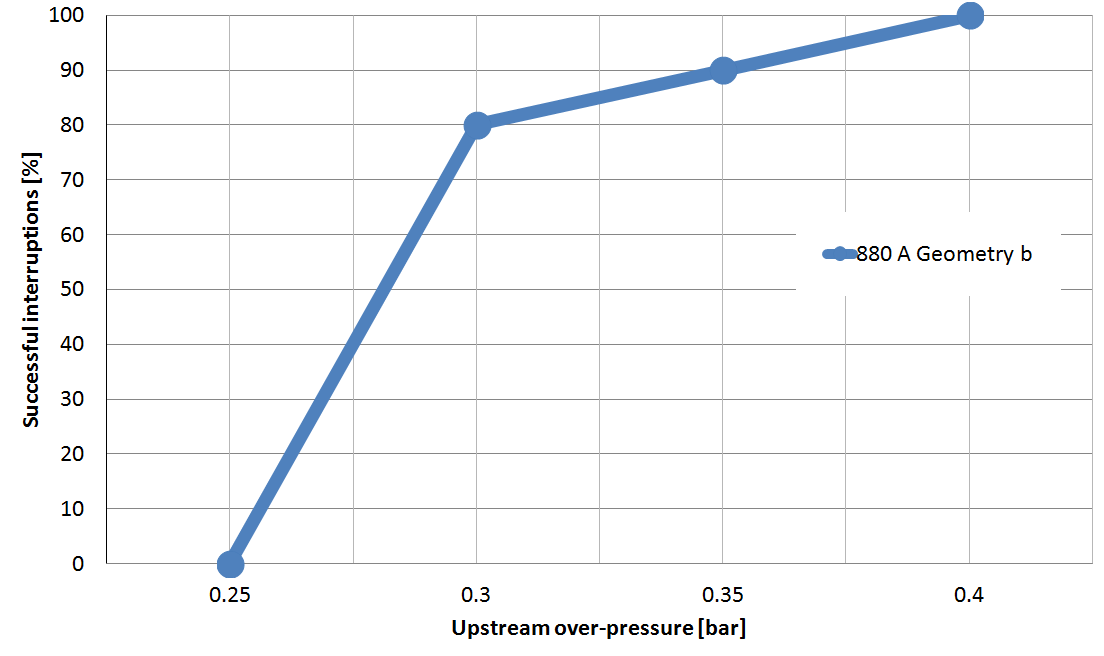
\includegraphics[scale=0.45]{Bilder/Results/geoB880amp.PNG}
\caption{Interruption test results for geometry \textbf{b} at 880 A when tests occurring "inside funnel" and "outside nozzle", and the results form the first and second CZ is added together.} \label{fig:results880AgeoB}
\end{figure}

\begin{figure}[H]
\centering
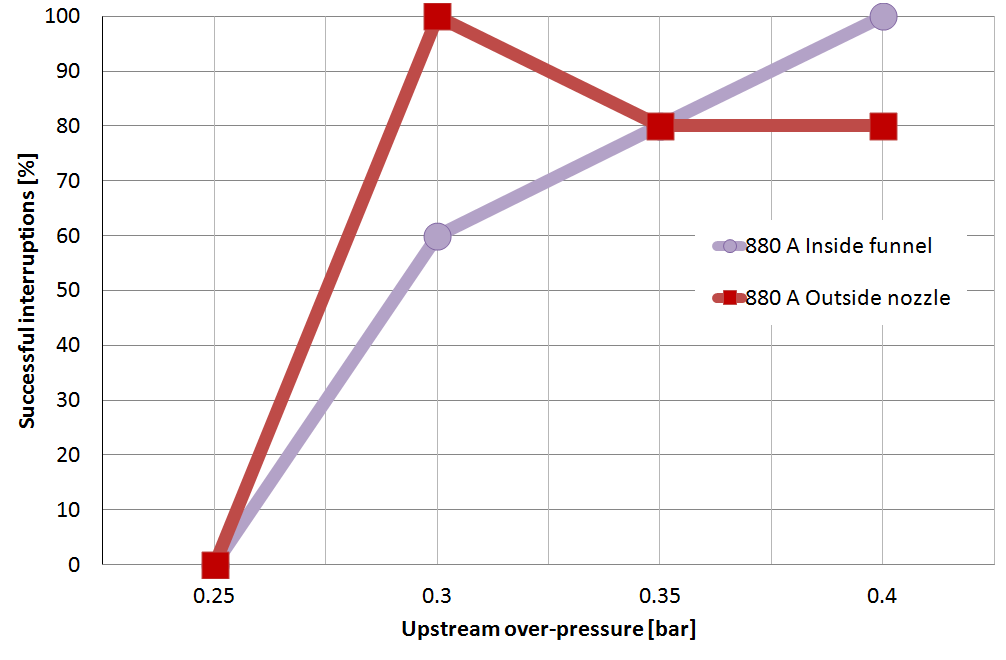
\includegraphics[scale=0.45]{Bilder/Results/geoB880ampcomp.PNG}
\caption{Interruption test results for geometry \textbf{b} at 880 A when only the first CZ is included and tests that occurred inside the funnel is separated from tests that occurred outside the nozzle.} \label{fig:results880AgeoBcomp}
\end{figure}

\subsubsection{Comparison and discussion of the test results for geometry \textbf{a} and \textbf{b}} \label{sec:compAandB}

In table \ref{tab:compgeoAandB} and figure \ref{fig:compgeoAandBAllcurrents} the results for the total interruption success rate for geometry \textbf{a} and geometry \textbf{b} are compared. As shown in the figure geometry \textbf{b} performed better than geometry \textbf{a} for the 880 A interruption test with a 50\% interruption success rate estimated to 0.28 bar over-pressure, while geometry \textbf{a} had a 50\% interruption success rate of 0.35 bar over-pressure. However, the 100\% interruption success rate was equal for both interruption tests at 0.4 bar over-pressure. For the 630 A interruption case geometry \textbf{b} had a better 50\% interruption success rate than geometry \textbf{a}. Both geometries interrupted the current successfully all the tests at 0.3 bar over-pressure, and interrupted 90\% of the tests at 0.25 bar over-pressure, resulting in almost an equal performance at the 630 A interruption test.

\begin{table}[h]
\center
\caption{Comparison of the interruption success rates for geometry \textbf{a} and \textbf{b}.}
\begin{tabular}{|l|c|c|c|c|c|c|}
\hline
\multirow{3}{*}{Geometry:} & \multicolumn{6}{|c|}{Interruption success rate}                                                           \\ \cline{2-7} 
                          & \multicolumn{3}{|c}{630 A interruption test}        & \multicolumn{3}{|c|}{880 A interruption test}       \\ \cline{2-7} 
                          & 0\% {[}bar{]} & 50\% {[}bar{]} & 100\% {[}bar{]} & 0\% {[}bar{]} & 50\% {[}bar{]} & 100\% {[}bar{]} \\ \hline
\textbf{a}                & 0.15           & 0.19            & 0.3              & 0.3            & 0.35            & 0.4              \\ \hline
\textbf{b}                & N/A            & 0.175           & 0.3              & 0.25           & 0.28            & 0.4              \\ \hline
\end{tabular}
\label{tab:compgeoAandB}
\end{table}

\begin{figure}[H]
\centering
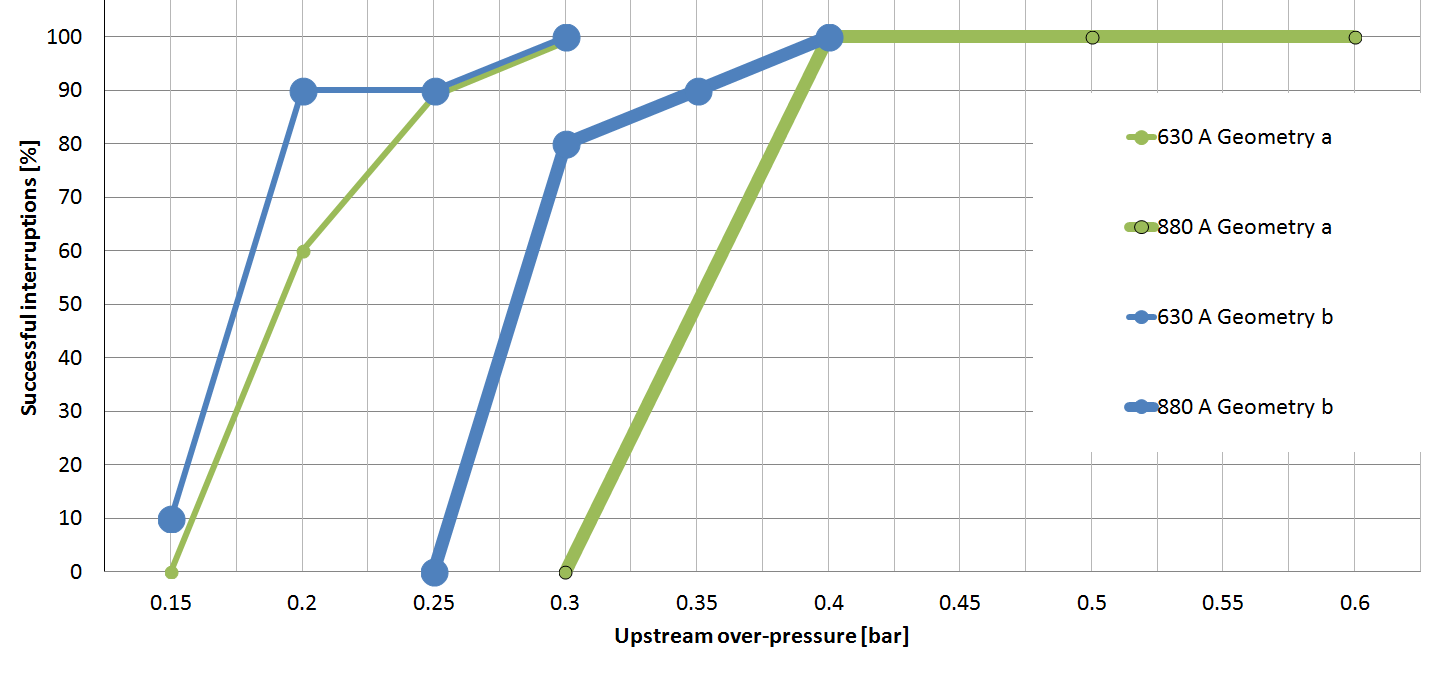
\includegraphics[scale=0.5, angle =90 ]{Bilder/Results/compGeoAandBNew2.PNG}
\caption{Comparison of the total interruption success rate for geometry \textbf{a} and \textbf{b} at 630 A and 880 A.} \label{fig:compgeoAandBAllcurrents}
\end{figure}

Previously conducted studies have shown that a short and narrow nozzle is preferred opposed to a long and wide one. The good performance of geometry \textbf{a} and \textbf{b} at 630 A was therefore as expected. As explained in section \ref{sec:testSwitchandContact} the nozzle for geometry \textbf{a} and \textbf{b} consists of two parts; a cylindrical part, with almost the same diameter as the contact pin, and one part shaped as a funnel at the end of the nozzle. Both parts are designed to obtain certain preferable air flow features during interruption as discussed in the paragraphs below.

During testing it became clear that the cylindrical part of the nozzle had an effect on the interruption success rate, since the interruption success rate decreased when the nozzle were starting to show signs of wear. Most of the wear on the nozzle were located in the cylindrical part, since this part was the most exposed to the stress from the arc. This wear resulted in an increase of the nozzle diameter, \textit{D}, which seems to be the cause of the decreasing interruption success rate.

One possible explanation for this wear caused decrease in interruption success rate for geometry \textbf{a} and \textbf{b}, as well as the good performance compared to wider nozzle designs, is how the air is replaced inside of the cylindrical part of the nozzle. In figure \ref{fig:twoNozzleDesignsNarrowandWideRep} a simplified example is presented. The figure shows a sketch over two nozzle designs during CZ, one wide nozzle (upper) and one narrow (lower). The blue area represents cold air, while the red area represents hot air. The tulip contact is marked with (1), and the nozzle is the grey area, marked with (2). The tulip contacts in the wide and narrow nozzle have the same contact area, and the pin is outside the nozzle at CZ. In the example it is assumed that the cold air from the pressure tank replaces the hot air heated by the arc by pushing it out of the nozzle, rather than mixing with it. In a more realistic scenario a combination of replacement and mixing of the air will occur. If the same upstream over-pressure is used for both nozzle designs, the same volume of hot air will be replaced. However, a wide nozzle have a bigger nozzle area than a narrow one, and this results in a longer distance for the arc to re-ignite between the tulip contact and the hot air zone in the narrow nozzle, making a re-ignition of the arc less likely.

\begin{figure}[H]
\centering
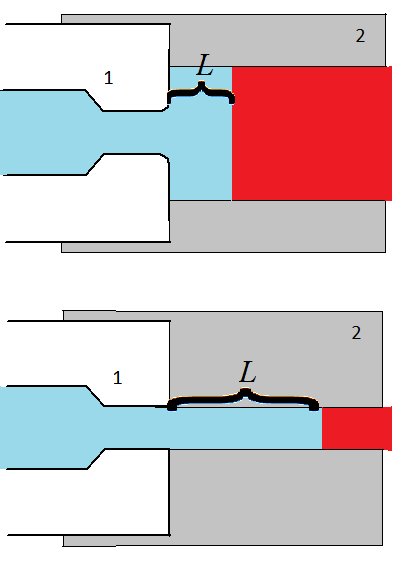
\includegraphics[scale=0.42]{Bilder/Results/nozzle_cooling_1.png}
\caption{Two nozzle designs, one wide (upper), and one narrow (lower). Illustration of how the re-ignition distance for the arc will increase when the same volume of hot air (red area) is replaced by cold air (blue area) inside of the two nozzle designs (not to scale).} \label{fig:twoNozzleDesignsNarrowandWideRep}
\end{figure}

If the simplified model explained above is extended to include a more realistic air flow scenario it will look like presented in figure \ref{fig:twoNozzleDesignsNarrowandWideRep_MIX}. The viscosity of the air flow is now included in the sketch. As can be seen in the figure two pockets of still, or rotating air can be seen between the tulip contact and nozzle wall, marked by orange triangular areas in the figure. In these regions the air will not be as efficiently replaced as in the rest of the nozzle, resulting in a higher concentration of ions and charged particles, as well as hotter air in than the cold area. The degree of air mixing will depend on how turbulent the flow is, which will increase with increasing pressure. As the figure shows, the distance the arc has to re-ignite in cold air will be even smaller than as presented in figure \ref{fig:twoNozzleDesignsNarrowandWideRep}. Even though the theory presented above is highly simplified, it might partially explain why a narrow nozzle is preferable to a wide nozzle. 
 

\begin{figure}[H]
\centering
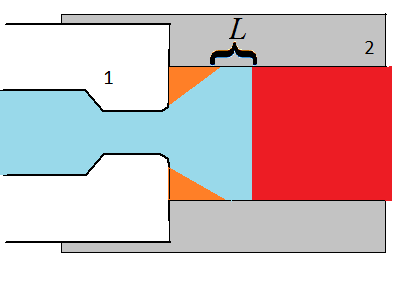
\includegraphics[scale=0.42]{Bilder/Results/nozzle_cooling_2_only_a.png}
\caption{The wide nozzle design from figure \ref{fig:twoNozzleDesignsNarrowandWideRep} when the viscosity of air is included (not to scale).} \label{fig:twoNozzleDesignsNarrowandWideRep_MIX}
\end{figure}

Another possible explanation for the good interruption success rate experienced for geometry \textbf{a} and \textbf{b} is that the narrow cylindrical nozzle section acted as an pressure chamber giving the test switch a small self blast function, as explained in section \ref{sec:puffer}. The diameter of the contact pin is almost equal the diameter of the nozzle, and the pin might partially clog the nozzle while inside the cylindrical part of it. This will make the cylindrical nozzle section into a pressure chamber.  When air gets heated by an arc, a pressure build-up will occur, since the air expands in a restricted volume. Due to this pressure build-up a short air blast might occur when the pin moves outside of the cylindrical part of the nozzle. If the air blast occurs in the right time, so that it cools the arc when it approaches CZ, the chance for re-ignition might be smaller, due to a more efficient removal of hot air. Thereby, resulting in a lower upstream over-pressure needed to successfully interrupt the current. 

In appendix \ref{app:SelfBlast}, a picture sequence of an air blast occurring during testing is presented for an 880 A interruption test for geometry \textbf{a}. The pre-set upstream over-pressure used was 0.3 bar. The first frame of the sequence show the moment right before the pin enters the funnel shaped part of the nozzle. Frame 2-14 shows the air blast, in the picture sequence every second frame was removed, so that the sequence would fit in one figure. The sequence was filmed with a frame rate of approximately 10 000 fps which resulted in a 2.5 ms time span for the air blast. After this time it is only the air flow generated by the pre-set pressure in the pressure tank that cools the arc.

Although this self blast effect is present in the picture sequence, its impact on the arc quenching abilities of the test switch is probably small. The duration of it is short, and for it to have any effect it is assumed that the CZ must occur right after it starts. For geometry \textbf{a} and \textbf{b} this will be when the pin is inside of the funnel part of the nozzle, but as presented in figure \ref{fig:results630AgeoAcomp}, \ref{fig:results630AgeoBcomp}, and \ref{fig:results880AgeoBcomp} no significant difference in the interruption success rate was found between "inside funnel" and "outside nozzle". Therefore, the effect of the observed air blast is assumed to not have had any significant impact on the interruption results performed in this experiment. To further understand and evaluate the impact of this self blast effect, more tests with a different nozzle design should be conducted. It is suspected that the effect of the air blast will depend on the RMS value of the current, as well as the volume of the pressure chamber. If the narrow cylindrical part of the nozzle is replaced with a bellow form, which have the same diameter at each end as the cylindrical part of geometry \textbf{a} and \textbf{b}, the effect of the volume in the pressure chamber can be more thoroughly analysed. It is possible that it exists an optimal volume and shape of the pressure chamber for a given current to maximise the pressure build-up in it, and thereby increasing the self blast effect so that it may will have a larger impact on the total interruption success rate.

During testing of geometry \textbf{a} and \textbf{b} two other phenomena were observed, which are assumed to have had an impact on the arc quenching abilities. In figure \ref{fig:funnelDisp} a comparison of the air flow in a short funnel shaped nozzle (upper) and a long cylindrical shaped nozzle (lower) is shown. The short funnel shaped nozzle is geometry \textbf{b} from this report and has an air flow formed as a drop with a tail, while the long cylindrical nozzle, which is geometry \textbf{c} from this report, has a more triangular formed air flow. It is possible that the air flow for geometry \textbf{b} is an advantage, since it might stabilise the arc, as well as cooling it more efficiently. This is because in the long cylindrical nozzle designs it has often been observed that the arc winds itself, causing unnecessary elongation of the arc. This elongation results in an increase of the arcing voltage as described in section \ref{sec:staticArcVoltage}, which will result in a higher energy dissipation and might set higher demands to the cooling mechanisms. Furthermore it seems like the drop formed air flow gives a more uniform and concentrated cooling along the whole length of the arc. The pictures are taken under fairly high current magnitudes far from CZ. This is because the air at CZ is not hot enough to be seen on the NIR camera, however, it is reasonable to assume that the air flow seen in the pictures would be obtained close to CZ, as well as at high currents. The two air flows shown in the figure below was taken under almost equal interruption conditions, and with the same camera settings. The current had an RMS value of 630 A, and had almost the same magnitude in the pictures. The arc had approximately the same length and an upstream over-pressure of 0.3 bar was used. The same air flow observed in geometry \textbf{b}, was observed for geometry \textbf{a} for all filmed interruption tests.

\begin{figure}[H]
\centering
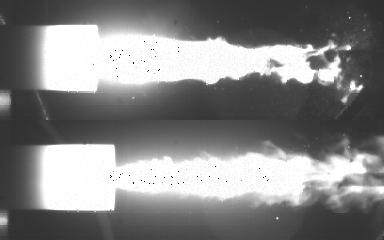
\includegraphics[scale=0.75]{Bilder/Results/compFunnelNormal.png}
\caption{Shape of the air flow during interruption testing for geometry \textbf{b} (upper) and geometry \textbf{c} (lower).} \label{fig:funnelDisp}
\end{figure}

The other phenomenon observed for the funnel shaped nozzle, which have not been observed in other interruption tests when using cylindrical shaped nozzles is a considerable milder peak in arcing voltage right before CZ, as shown in figure \ref{fig:mildFunnelArcVlotage}. It is possible that the milder arcing voltage observed for geometry \textbf{a} and \textbf{b} is linked with the different air flow discussed above, however, this link is yet to be confirmed.

\begin{figure}[H]
\centering
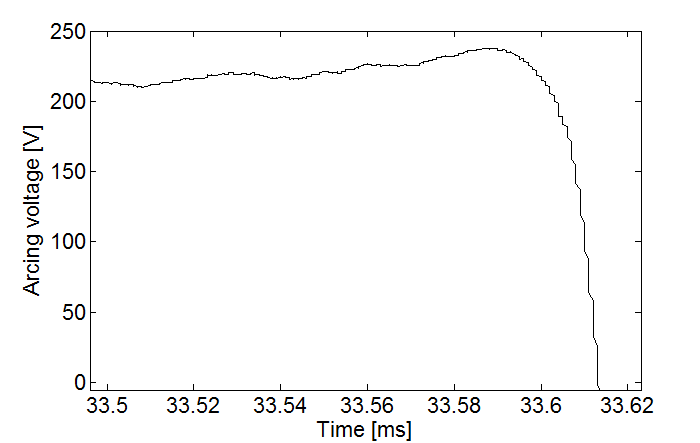
\includegraphics[scale=0.5]{Bilder/Results/funnelArcDrop.PNG}
\caption{Arcing voltage for geometry \textbf{b} the last 100 $\mu$s before CZ during a successful 630 A interruption test.} \label{fig:mildFunnelArcVlotage}
\end{figure}

Figure \ref{fig:mildFunnelArcVlotage} shows a 630 A interruption test for geometry \textbf{b}, with an upstream over-pressure of 0.3 bar. The arc was successfully interrupted at the second CZ, which occurred when the pin contact was 73 mm from the female contact. This arcing voltage shape, was observed for both geometry \textbf{a} and \textbf{b}, and occurred in nearly all of the interruption tests performed for every current level. In figure \ref{fig:75mmSuccessful} from section \ref{sec:arcingVoltageSuccessFulandUnsuccessfulResults} in this report, four successful interruptions for geometry \textbf{c} can be seen, with the same interruption conditions as the one presented in the figure above. If the two figures are compared it is clear that the arcing voltage is much higher during this time span for geometry \textbf{c}. For geometry \textbf{c} the arcing voltage starts at approximately 300 V, and steadily increases up to approximately 400 V. For the tests presented for geometry \textbf{b} in figure \ref{fig:mildFunnelArcVlotage}, the arcing voltage starts at 200 V, and rises to a peak of only 235 V. The result is a considerable lower dissipated energy for geometry \textbf{a} and \textbf{b}, if compared to a long cylindrical geometry, like geometry \textbf{c}, since the current magnitude it equal and unaffected of the arcing voltage. As argued in section \ref{sec:TherMalReConsid}, a low amount of dissipated energy close to CZ will most likely result in an easier interruption, as seen for geometry \textbf{a} and \textbf{b}, when compared to other previously tested cylindrical nozzle geometries.

In the paragraph above some theories and observed differences between the funnel shaped nozzles and previously tested cylindrical shaped nozzles are presented. It is however, not clear if it is the narrow cylindrical part or the funnel shape at the end of the nozzle which had the biggest impact on the good interruption success rate for geometry \textbf{a} and \textbf{b}. Therefore, further experiments with a nozzle design equal to geometry \textbf{a} and \textbf{b}, but without the funnel part of the nozzle should be conducted. Then the impact of the narrow cylindrical part of the nozzle on the interruption success rate can be found, and used to evaluate the effect of the funnel shaped part of the nozzle. 

The 880 A interruption test for geometry \textbf{a} and \textbf{b} also performed well and as expected when compared to previously tested geometries. Both the interruption theories presented above for the 630 A interruption test, are still considered as possible explanations for the good interruption success rate at 880 A. The 880 A tests showed similar air flows as in figure \ref{fig:funnelDisp}, and the mild arcing voltage presented in figure \ref{fig:mildFunnelArcVlotage} was also present.

The variation between geometry \textbf{a} and \textbf{b} at 880 A, where geometry \textbf{b} had a better interruption rate at most pressure levels was also as expected. This can be explained by the volume flow of air that is larger though geometry \textbf{b} at a given upstream over-pressure. The volume flow $(Q)$ is defined by equation \eqref{eq:volumeFlow}, which states that the volume flow depends on the velocity of the air flow $(v)$, as well as the cross-section area $(A)$ it is flowing through. The velocity of the air flow can be obtained from Bernoulli's equation. If the air flow is simplified to be incompressible and inviscid, the velocity of the air flow will only depend on the over-pressure in the pressure tank. The velocity found with Bernoulli's equation is the maximum speed of the air flow, which will occur in the narrowest part of the geometry. For geometry \textbf{a} and \textbf{b}, this is inside of the tulip contact when the pin is outside of the nozzle at the moment of interruption.

If the air flow is simplified to be regarded as incompressible, it can be assumed that the volume flow of air must be conserved though the tulip contact and the nozzle. Given this assumption the velocity of the air flow inside of the nozzle can be calculated as shown in equation \eqref{nozzle_speed} below.

\begin{equation} \label{nozzle_speed}
\begin{split}
Q=v_{nozzle} A_{nozzle}=v_{tulip} A_{contact} \\
v_{nozzle}=v_{tulip} \left( \frac{d}{D} \right) ^2 \ \ \ \ \ \ \ \ \
\end{split}
\end{equation} 

As shown in table \ref{tab:contGeoPara} from section \ref{sec:testSwitchandContact}, $D/d$ is equal for both geometry \textbf{a} and \textbf{b}, resulting in the same velocity of the air flow at a given pressure for the two geometries. Therefore, the only difference between the two geometries is the volume flow of air, that is larger for geometry \textbf{b}, which is an advantage when interruption currents. However, it should be noted that the assumption of an incompressible and inviscid air flow is probably not true, since turbulence, wall effects, and variation in density and temperature is likely to be present. Despite these effects, it is likely that the parameter that has the biggest impact on the current interruption abilities between the two geometries is the volume flow passing through it.

Furthermore, empirical data collected from this, and previously conducted tests has provided a sketch illustrating the relationship between the upstream over-pressure and the area of the contacts needed to obtain an 50\% interruption success rate, shown in figure \ref{fig:sketch50Intrate}. As described from this empirical model seen in the figure below, a rather small increase in over-pressure is needed to obtain an equal interruption rate for geometry \textbf{a} and geometry \textbf{b} for 630 A, but for 880 A a considerable increase in pressure is expected. Given this model, the variance between the two geometries at the 880 A interruption tests, and the equal interruption rate at 630 A was as expected.

\begin{figure}[H]
\centering
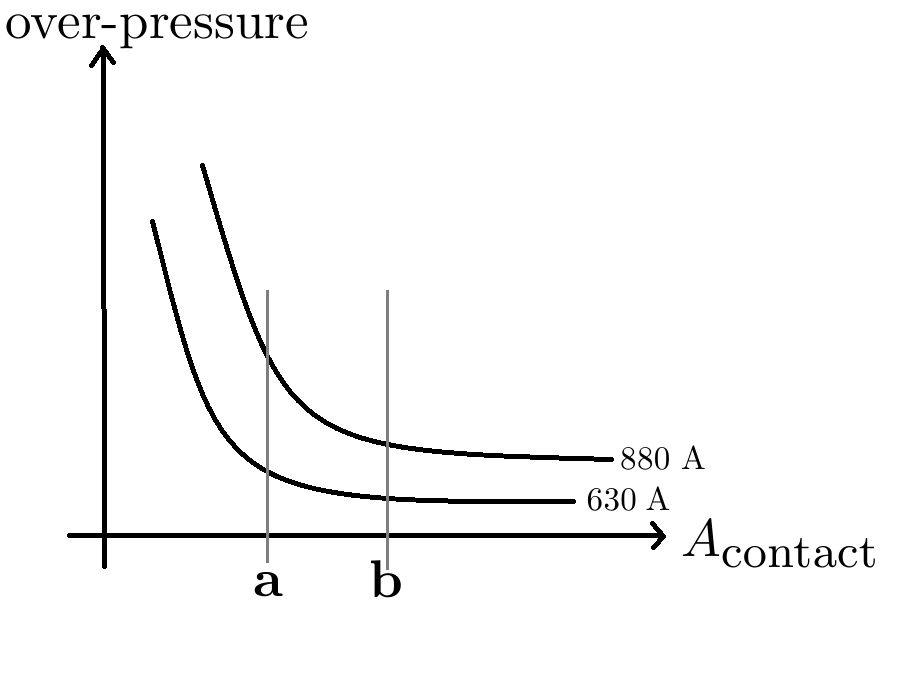
\includegraphics[scale=0.45]{Bilder/Results/pressureVSAcontact2.png}
\caption{Relationship between contact area and upstream over-pressure used to obtain 50\% interruption success rate for two different currents (schematically).} \label{fig:sketch50Intrate}
\end{figure}

When choosing a contact geometry for a commercial switchgear design several parameters must be addressed, so that the total costs of the switchgear is minimised, while good functionality and lifespan is obtained. In the experimental set-up used in this report, a 6 litre tank is used to provide an almost constant pressure throughout the whole interruption process. In a commercial switchgear based on the puffer design, the puffer volume is limited and the pressure will vary with time, as described in section \ref{sec:puffer}. An increase in volume flow is strongly linked with an increase in contact area, like between geometry \textbf{a} and \textbf{b}. To obtain a sufficient pressure in the puffer volume throughout the interruption process by increasing the contact area, a stronger spring to drive the piston can be used. But a stronger spring requires a more powerful motor to load it after use, which uses more space and adds to the expenses of the switchgear. Furthermore, a bigger contact area will decrease the time the piston will use to empty the puffer volume, so that the puffer might not cover enough CZ crossings before it is empty of pressurised air. To adjust for this the volume of the puffer can be increased, which will add to the size of the switchgear. To the contrary a too small contact might not give a sufficient air flow, even at fairly high pressures, as explained by figure \ref{fig:sketch50Intrate}. Another problem which can arise if the contact area is too small and sharp is dielectric flash overs when the switch is open due to voltage transients, or welding under closing operation. Copper-wolfram, which the contact members are made of, is also an expensive metal, and by using a smaller contact geometry the total costs of the switch might be lowered. This means that a geometry that needs a high upstream over-pressure to successfully interrupt a current is not necessarily unsuited for a switchgear design, as long as the needed pressure is obtainable. Therefore, the choice of contact size can be considered as a trade-off between available space, motor power and total costs.

\subsubsection{Interruption results for geometry \textbf{c}} \label{sec:intTestGeoC}

\subsubsection*{630 A interruption tests}
In figure \ref{fig:results630AgeoC}, the total interruption success rate for the 630 A test for geometry \textbf{c} is presented. Each data point consists of 5 interruption tests, except for the tests performed at 0.3 bar upstream over-pressure where 10 interruption test was conducted. For all the tests the first CZ occurred outside of the nozzle. The extra five tests performed at 0.3 bar was conducted because the initial five tests at 0.3 bar had a 100\% interruption success rate, but since all the tests at 0.25 bar over-pressure failed it was suspected that the results at 0.3 bar were inaccurate. Five new tests at 0.3 bar were conducted and the interruption success rate decreased. After this adjustment, the normal test procedure was followed and new tests where conducted at a higher pressure level.

After the test procedure was adjusted as described above the 100\% interruption success rate occurred at an upstream over-pressure of 0.4 bar. Other key values from the interruption tests can be seen in table \ref{tab:compgeoCandD}.

\begin{figure}[H]
\centering
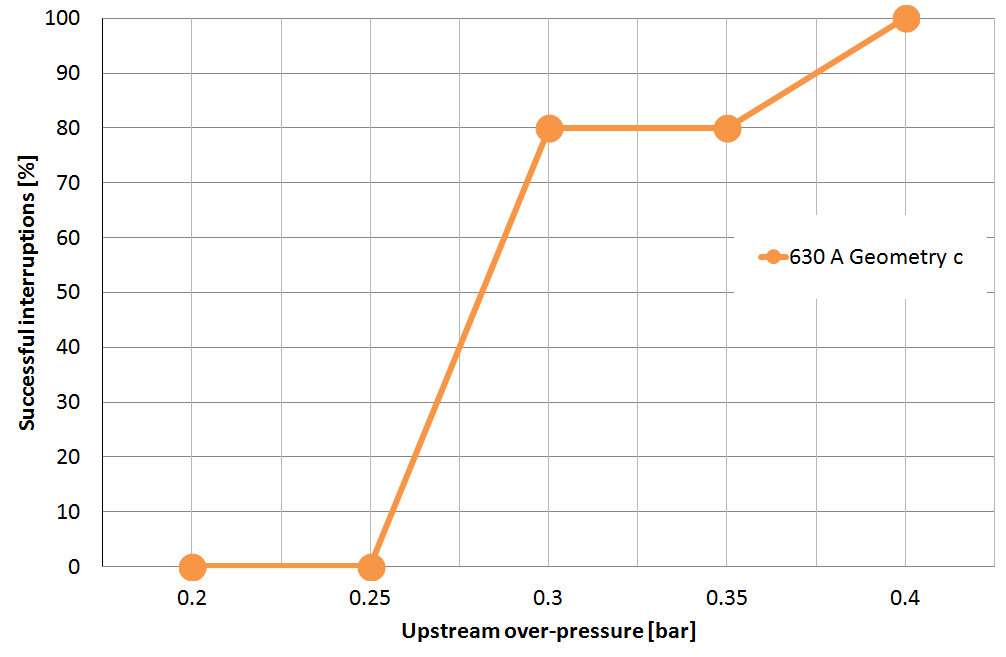
\includegraphics[scale=0.45]{Bilder/Results/geoC630amp.PNG}
\caption{Interruption test results for geometry \textbf{c} at 630 A when tests occurring "outside nozzle", and the results from the first and second CZ are added together.} \label{fig:results630AgeoC}
\end{figure}

\subsubsection*{880 A interruption tests}
In figure \ref{fig:results880AgeoC}, the total interruption success rate for the 880 A test for geometry \textbf{b} is presented. Each data point consists of 5 interruption tests and for all the tests the first CZ occurred outside of the nozzle. Key values from the interruption tests can be seen in table \ref{tab:compgeoCandD}. 

%As seen from figure \ref{fig:results880AgeoC} the 100\% interruption success rate occurred at a upstream over-pressure of 0.5 bar, while none interruptions where obtained at 0.35 bar upstream over-pressure. The 50\% interruption success rate can be obtained from the figure, and corresponds to an over-pressure of 0.425 bar.

\begin{figure}[H]
\centering
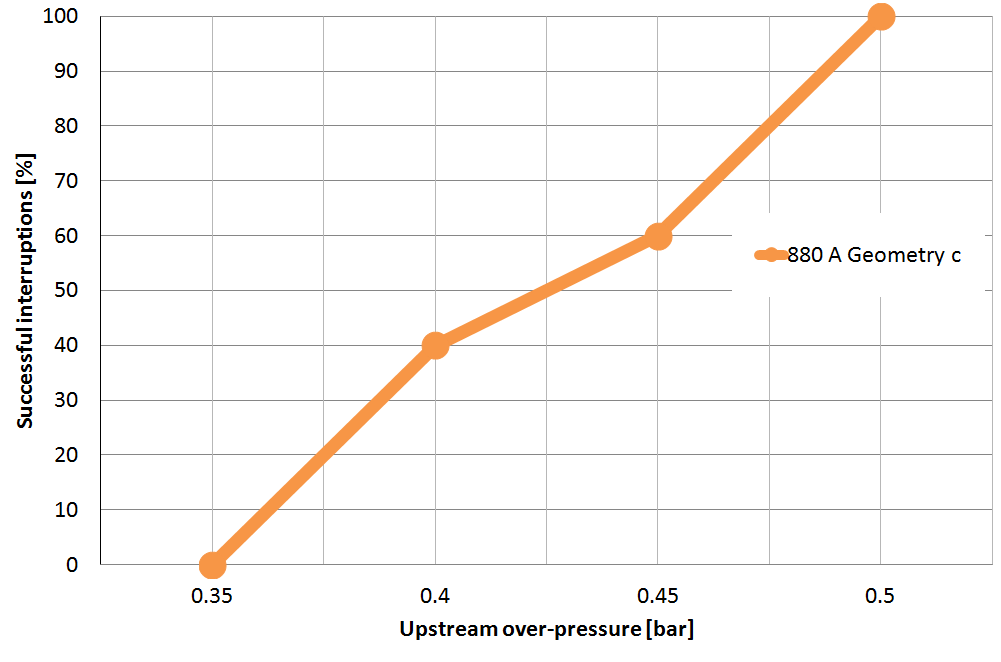
\includegraphics[scale=0.45]{Bilder/Results/geoC880amp.PNG}
\caption{Interruption test results for geometry \textbf{c} at 880 A when tests occurring "inside funnel" and "outside nozzle", and the results from the first and second CZ are added together.} \label{fig:results880AgeoC}
\end{figure}

\subsubsection{Comparison and discussion of the test results for geometry \textbf{c} and \textbf{d}}

As stated in section \ref{sec:testSwitchandContact}, geometry \textbf{c} is going to be compared to a previously tested geometry, denoted \textbf{d}. Geometry \textbf{d} was tested by Nina Sasaki Aanensen and the results will be published in the article: "Air flow investigation for a medium voltage load break switch" \cite{bib:AFIMVLBA} (In that article geometry \textbf{d} was denoted as geometry \textbf{a}). In this article only the first CZ was included in the presented results and each data point consists of ten interruption tests. To be comparable to geometry \textbf{c} the interruption results for geometry \textbf{d} has been extended, so that the second CZ is included in the interruption results for geometry \textbf{d} in this report. In figure \ref{fig:compgeoCandDAllcurrents} a comparison of the total interruption success rate for geometry \textbf{c} to the previously tested geometry \textbf{d} can be seen.

%However, it seems beneficial for the readability of the report to present the results from the previously tested geometry \textbf{d} and geometry \textbf{c} in the same figure. Therefore, a comparison of the total interruption success rate for geometry \textbf{c} to the previously tested geometry \textbf{d} are shown in figure \ref{fig:compgeoCandDAllcurrents}.

Figure \ref{fig:compgeoCandDAllcurrents} shows that geometry \textbf{d} performed somewhat better than geometry \textbf{c} for the 630 A interruption tests. Geometry \textbf{d} interrupted all the tests at 0.3 bar over-pressure, while geometry \textbf{c} had a 100\% interruption success rate at 0.4 bar over-pressure. Geometry \textbf{c} had none successful interruptions at 0.25 bar over-pressure, while geometry \textbf{d} had a 0\% interruption success rate at 0.2 bar over-pressure. The 50\% interruption success rate for geometry \textbf{c} was estimated to 0.28 bar over-pressure and geometry \textbf{d} had a 50\% interruption success rate at approximately 0.26 bar over-pressure.

For the 880 A current interruption test, geometry \textbf{c} was considerably better than geometry \textbf{d}. Geometry \textbf{c} interrupted all the tests at 0.5 bar over-pressure, which was the same pressure level where geometry \textbf{d} only successfully interrupted 40\% of the tests, this was also the lowest tested pressure for geometry \textbf{d}. Geometry \textbf{d} had a 100\% interruption success rate at 0.6 bar over-pressure, and a 50\% interruption success rate at about 0.52 bar over-pressure. Where geometry \textbf{c} failed all the interruptions at 0.35 bar over-pressure and had a 50\% interruption success rate estimated to 0.425 bar over-pressure.

In table \ref{tab:compgeoCandD} a summary of the performance of geometry \textbf{c} compared to geometry \textbf{d} can be seen.

\begin{table}[h]
\center
\caption{Comparison of the interruption success rates for geometry \textbf{c} and geometry \textbf{d}.}
\begin{tabular}{|l|c|c|c|c|c|c|}
\hline
\multirow{3}{*}{Geometry:} & \multicolumn{6}{|c|}{Interruption success rate}                                                           \\ \cline{2-7} 
                          & \multicolumn{3}{|c}{630 A interruption test}        & \multicolumn{3}{|c|}{880 A interruption test}       \\ \cline{2-7} 
                          & 0\% {[}bar{]} & 50\% {[}bar{]} & 100\% {[}bar{]} & 0\% {[}bar{]} & 50\% {[}bar{]} & 100\% {[}bar{]} \\ \hline
\textbf{c}                & 0.25           & 0.28            & 0.4              & 0.35            & 0.425            & 0.5              \\ \hline
\textbf{d}                & 0.2            & 0.26           & 0.3              & N/A           & 0.52            & 0.6              \\ \hline
\end{tabular}
\label{tab:compgeoCandD}
\end{table}

\begin{figure}[H]
\centering
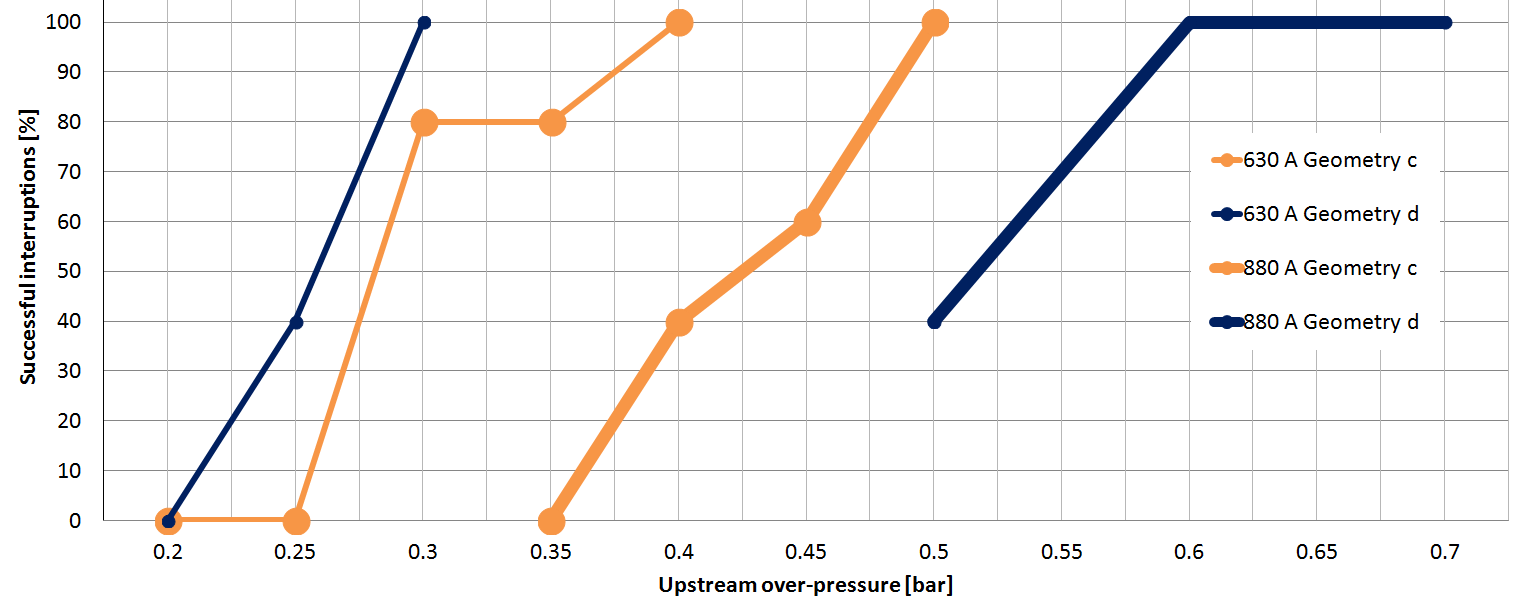
\includegraphics[scale=0.5, angle =90 ]{Bilder/Results/compGeoCandDNew.PNG}
\caption{Comparison of the total interruption success rate for geometry \textbf{c} and geometry \textbf{d} at 630 A and 880 A.} \label{fig:compgeoCandDAllcurrents}
\end{figure}

For the 880 A test, the results are like expected. As explained by figure \ref{fig:sketch50Intrate} it was assumed that a considerably lower pressure was needed to interrupt the current when the contact diameter increases, as from geometry \textbf{c} to \textbf{d}. The same trend was observed between geometry \textbf{a} and \textbf{b} at the 880 A interruption test.

In the 630 A interruption test, geometry \textbf{d} performed marginally better than geometry \textbf{c}. Given the empirical model from figure \ref{fig:sketch50Intrate}, which is based on previously conducted experiments, it is reasonable to assume that these two geometries performed almost equal at 630 A. The small difference in the results between them can be due to the limited amount of tests conducted at each pressure level. In section \ref{sec:impactOfTestNumber} the impact on the total interruption success rate when increasing the number of tests at each pressure level is more thoroughly investigated. It should be noted that a somewhat better performance of geometry \textbf{d} compared to other larger contact geometries at 630 A have been observed in previously conducted tests. This will be explained further in the article: "Air flow investigation for a medium voltage load break switch" \cite{bib:AFIMVLBA}.

%This is not as expected considering that the volume flow of air is larger though geometry \textbf{c} at a given upstream over-pressure. The volume flow $(Q)$ is defined by equation \eqref{eq:volumeFlow}, which states that the volume flow depends on the velocity of the air flow $(v)$, as well as the cross-section area $(A)$ it is flowing through. The velocity of the air flow can be obtained from Bernoulli's equation. If the air flow is simplified to be incompressible and inviscid, the velocity of the air flow will only depend on the over-pressure in the pressure tank. The velocity found with Bernoulli's equation is the maximum speed of the air flow, which will occur in the narrowest part of the geometry. For geometry \textbf{c} and \textbf{d}, this is inside of the tulip contact, since the pin is outside of the nozzle at the moment of interruption for all of the tests.

%If the air flow is simplified to be regarded as incompressible, it can be assumed that the volume flow of air must be conserved though the tulip contact and the nozzle. Given this assumption the velocity of the air flow inside of the nozzle can be calculated as shown in equation \eqref{nozzle_speed} below.

%\begin{equation} \label{nozzle_speed}
%\begin{split}
%Q=v_{nozzle} A_{nozzle}=v_{tulip} A_{contact} \\
%v_{nozzle}=v_{tulip} \left( \frac{d}{D} \right) ^2 \ \ \ \ \ \ \ \ \
%\end{split}
%\end{equation} 

%As shown in table \ref{tab:contGeoParaC} from section \ref{sec:testSwitchandContact}, $D/d$ is equal for both geometry \textbf{c} and \textbf{d}, resulting in the same velocity of the air flow at a given pressure for the two geometries. Therefore, the only difference between the two geometries is the volume flow of air, that is larger for geometry \textbf{c}, which is an advantage when interruption currents. However, it should be noted that the assumption of an incompressible and inviscid air flow is probably not true, since turbulence, wall effects, and variation in density and temperature is likely to be present. But despite these effects, it is likely that the parameter that has the biggest impact on the current interruption abilities between the two geometries is the volume flow passing through it.

%Given the empirical model from figure \ref{fig:sketch50Intrate}, which is based on previously conducted experiments and that the only difference between geometry \textbf{c} and \textbf{d} are the volume flow, it is reasonable to assume that these geometries performed almost equal at 630 A, and that the small difference in the results between them is due to the limited amount of tests conducted at each pressure level. In section \ref{sec:impactOfTestNumber} the impact on the total interruption success rate when increasing the number of tests at each pressure level is more thoroughly investigated.

\subsubsection{Uncertainties related to the number of tests in a data point} \label{sec:impactOfTestNumber}
Due to an unknown latency in the release mechanism of the test switch it was hard to adjust the pin's x-position so that it occurred in the desired region at the moment of CZ. Therefore, an excessive amount of tests had to be performed at some pressure levels. Some of these extra tests have been included in table \ref{tab:successrate1} and \ref{tab:successrate2} as "Success rate based on all performed tests". These tests include more than just the ten first tests, as described by the test procedure in section \ref{sec:procedure}. This can be used to check if ten tests at each pressure level is good enough to describe the actual interruption success rate, or if more tests should be conducted in future experiments. It will also describe the reliability of the results obtained in this report.

In table \ref{tab:successrate1} all tests that occurred inside of the funnel or outside of the nozzle is included as a base for the "Success rate based on all performed tests". For the results shown in table \ref{tab:successrate2} all the tests that occurred outside of the nozzle is included for the "Success rate based on all performed tests", except those that occurred in the boundary region between outside and inside of the nozzle. The results presented in both tables are interpreted as described by figure \ref{fig:flowchart}, and all the tests are collected using a current of 630 A for the interruption test. 

When increasing the number of conducted tests at a pressure level the total interruption success rate changes from when applying only ten tests, except for the 0.3 bar over-pressure test for geometry \textbf{a} where all the test were successfully interrupted for all performed tests. For geometry \textbf{a} at 0.25 bar there is a difference of: 77.8\%-90\%=12.2\%, between the success rate for all the performed tests and the first ten tests. This difference is 5\% for geometry \textbf{c} at 0.3 bar over-pressure. Therefore, the results presented in section \ref{sec:interruptionTests} of this report should not be regarded as absolute limits, since there are uncertainties connected with the obtained numbers. It is suspected that these uncertainties are mostly caused by the limited number of tests performed at each pressure level, but other factors like contact wear and nozzle deformation might also be partially responsible. The interruption test results are mainly used to compare geometries to each other. For this purpose the variation above is acceptable, as long as the variation is taken into account for when comparing the results. However, ten tests are probably the lowest number of tests that should be used for each pressure level. In some interruption cases only five tests have been used at each pressure level, like for geometry \textbf{c} in this report (except for 0.3 bar over-pressure, where the test procedure was altered). This small number of tests makes room for interpretation errors in the results, as well as a weaker foundation for strong conclusions in the experimental work. Furthermore, large uncertainties related to the interruption results might make them more difficult to use for mathematical purposes, like if simulating the interruption chance for a contact geometry at a given pressure. It should also be noted that it seems like the 0\% and 100\% interruption success rate have less variation than the interruption success rates in between. This is probably because these are at close to the limiting values, and therefore makes lesser room for variation.

\begin{table}[H]
\center
\caption{Interruption success rate for geometry \textbf{a} at 630 A.}
\begin{tabular}{|c|c|c|c|}
\hline 
Upstream & Number of tests & Success rate based & Success rate based \\ over-pressure [bar] &  performed in total &  on all performed tests [\%] &  on test procedure [\%] \\ 
\hline 
0.25 & 18 & 77.8 & 90 \\ 
\hline 
0.3 & 18 & 100 & 100 \\ 
\hline 
\end{tabular} 
\label{tab:successrate1}
\end{table}

\begin{table}[H]
\center
\caption{Interruption success rate for geometry \textbf{c} at 630 A.}
\begin{tabular}{|c|c|c|c|}
\hline 
Upstream & Number of tests & Success rate based & Success rate based \\ over-pressure [bar] &  performed in total &  on all performed tests [\%] &  on test procedure [\%] \\ 
\hline 
0.3 & 24 & 75 & 80 \\ 
\hline  
\end{tabular} 
\label{tab:successrate2}
\end{table}


\newpage
\subsection{Arcing voltage between successful and unsuccessful interruptions} \label{sec:arcingVoltageSuccessFulandUnsuccessfulResults}
For geometry \textbf{c} the arcing voltage was recorded and saved during the 630 A interruption tests at an over-pressure of 0.3 bar to see if a difference in arcing voltage could be observed between successful and unsuccessful interruptions. Two test series where conducted, one where the second CZ crossing occurred when the pin was positioned at x=75 mm, and one when the pin's position was inside the nozzle, at x=18 mm. The data presented in this section has been processed in matlab, where the arcing voltage has been smoothed to remove measuring noise and aligned so that the successful or unsuccessful current interruptions have the CZ at the same x-axis position. All the plots consist of data from the last 100 $\mu$s before the CZ, since this is, as argued in section \ref{sec:TherMalReConsid}, the most crucial time span to determine if a thermal re-ignition is to occur or be avoided.

For the test series with the second CZ crossing occurring at x=75 mm, nine interruption tests were performed in total. Five tests experienced a thermal re-ignition, and four tests successfully interrupted the current at the second CZ. As described in section \ref{sec:staticArcVoltage} the length of the arc influences the arcing voltage, therefore interruption attempts that was not in the area of interest (x=75 $\pm$ 3 mm) were discarded. Even though many tests where conducted, it was not obtained five successful interruption with the right pin position, which was the intended test procedure. This resulted in that only four successful interruption tests are included in the data collection for this arcing voltage test.

Figure \ref{fig:75mmUnSuccessful} shows the arcing voltage for the five interruption tests where a thermal re-ignition occurred at the second CZ, which was placed at approximately x=75 mm. The four successful current interruption tests with this length of the arc are displayed in figure \ref{fig:75mmSuccessful}. In appendix \ref{app:pictureSeq75mm}, picture sequences of the arc from the moment right before and after CZ for the nine arcing voltage tests presented in figure \ref{fig:75mmUnSuccessful} and \ref{fig:75mmSuccessful} can be seen.

\begin{figure}[H]
\centering
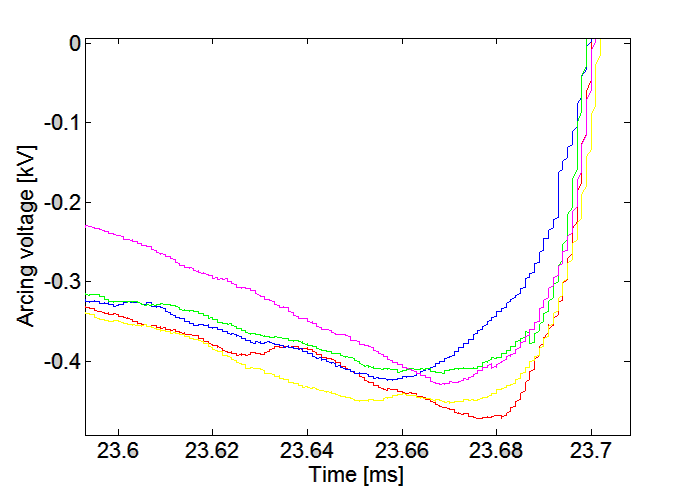
\includegraphics[scale=0.6, angle =0 ]{Bilder/Results/ArcingVoltage_75_reIgnition.PNG}
\caption{The arcing voltage for five interruption tests at 0.3 bar over-pressure and a current of 630 A. All the five tests experienced a thermal re-ignition at the second CZ, which occurred at approximately  x=75 mm.} \label{fig:75mmUnSuccessful}
\end{figure}

\begin{figure}[H]
\centering
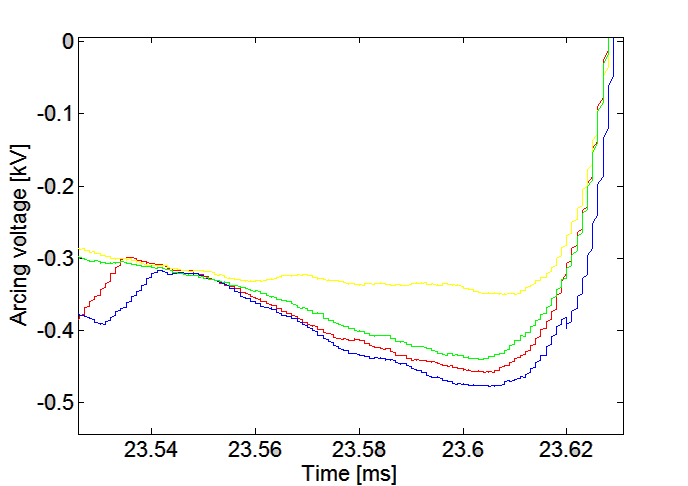
\includegraphics[scale=0.6, angle =0 ]{Bilder/Results/ArcingVoltage_75_none_reIgnition.PNG}
\caption{The arcing voltage for four interruption tests at 0.3 bar over-pressure and a current of 630 A. All the four tests was interrupted successfully at the second CZ, which occurred at approximately  x=75 mm.} \label{fig:75mmSuccessful}
\end{figure}

Based on the results presented in figure \ref{fig:75mmUnSuccessful} and \ref{fig:75mmSuccessful}, the average arcing voltage (blue line) for the five unsuccessful and the four successful current interruptions were calculated and presented in figure \ref{fig:75mmUnSuccessful_ave} and \ref{fig:75mmSuccessful_ave}. The two interruption tests from each of the two data collections which had the largest (green line) and smallest (red line) arcing voltage from the average arcing voltage are plotted together with it.

In figure \ref{fig:75mm_both_ave} the two average arcing voltages from figure \ref{fig:75mmUnSuccessful_ave} and \ref{fig:75mmSuccessful_ave} are plotted together. The green line is the average arcing voltage where the thermal re-ignitions occurred, while the magenta line is the average arcing voltage for the successful interruptions.

\begin{figure}[H]
\centering
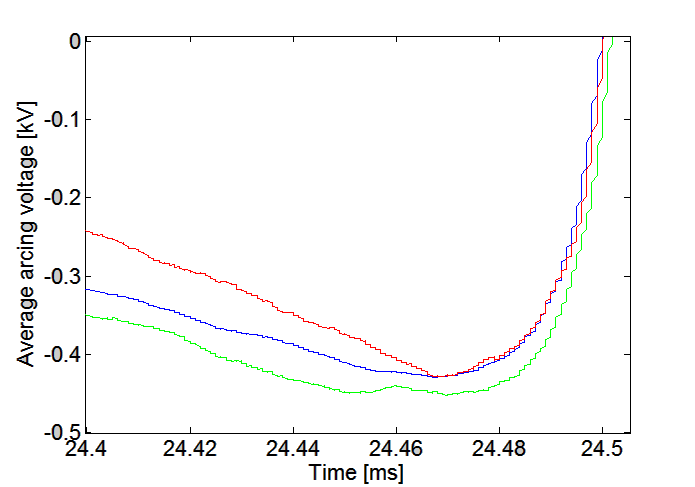
\includegraphics[scale=0.6, angle =0 ]{Bilder/Results/ArcingVoltage_75_reIgnition_average.PNG}
\caption{The average arcing voltage (blue line) for the five interruption tests at 0.3 bar over-pressure and a current of 630 A, together with the lowest (red line) and highest (blue line) arcing voltages obtained during testing. All the five tests experienced a thermal re-ignition at the second CZ, which occurred at approximately  x=75 mm.} \label{fig:75mmUnSuccessful_ave}
\end{figure}

\begin{figure}[H]
\centering
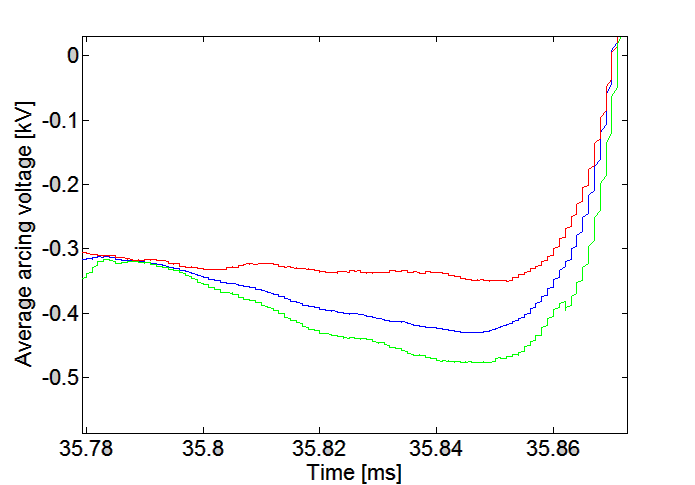
\includegraphics[scale=0.6, angle =0 ]{Bilder/Results/ArcingVoltage_75_none_reIgnition_average.PNG}
\caption{The average arcing voltage (blue line) for the four interruption tests at 0.3 bar over-pressure and a current of 630 A, together with the lowest (red line) and highest (blue line) arcing voltages obtained during testing. All the four tests where interrupted successfully at the second CZ, which occurred at approximately  x=75 mm.} \label{fig:75mmSuccessful_ave}
\end{figure}

\begin{figure}[H]
\centering
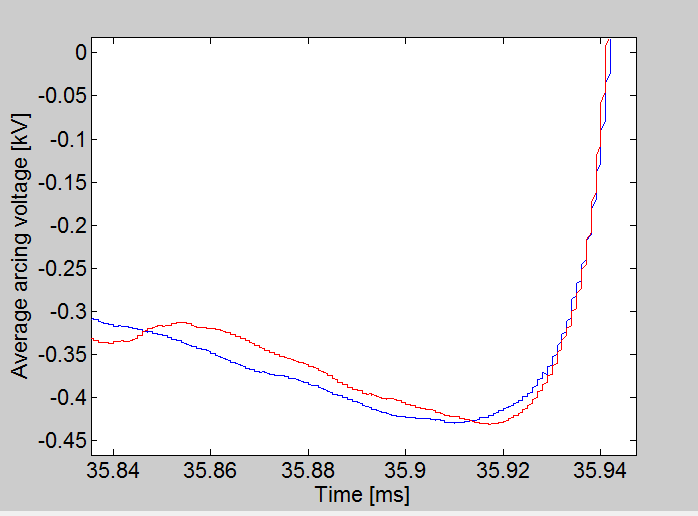
\includegraphics[scale=0.6, angle =0 ]{Bilder/Results/ArcingVoltage_75_both_average.PNG}
\caption{The average arcing voltage for both the successful (magenta line) and unsuccessful (green line) interruption tests.} \label{fig:75mm_both_ave}
\end{figure}

For the test series with the first CZ occurring at a pin position of x=18 mm, ten interruption tests were performed in total. Five tests had a thermal re-ignition, and the other five tests successfully interrupted the current at the first CZ. As previously stated in section \ref{sec:staticArcVoltage} the length of the arc influences the arcing voltage, therefore interruption attempts that was not in the area of interest (x=18 $\pm$ 3 mm) were discarded.

In figure \ref{fig:18mmUnSuccessful} the arcing voltage for five of the interruption tests are shown, all the five tests experienced a thermal re-ignition at the first CZ, which occurred at approximately x=18 mm. The five interruption tests which successfully interrupted the current are displayed in figure \ref{fig:18mmSuccessful}.

\begin{figure}[H]
\centering
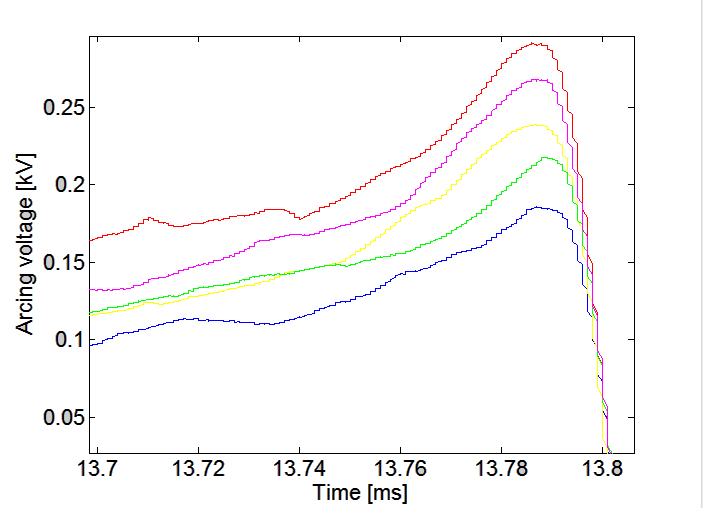
\includegraphics[scale=0.6, angle =0 ]{Bilder/Results/ArcingVoltage_18_reIgnition.PNG}
\caption{The arcing voltage for five interruption tests at 0.3 bar over-pressure and a current of 630 A. All the five tests experienced a thermal re-ignition at the second CZ, which occurred at approximately  x=18 mm.} \label{fig:18mmUnSuccessful}
\end{figure}

\begin{figure}[H]
\centering
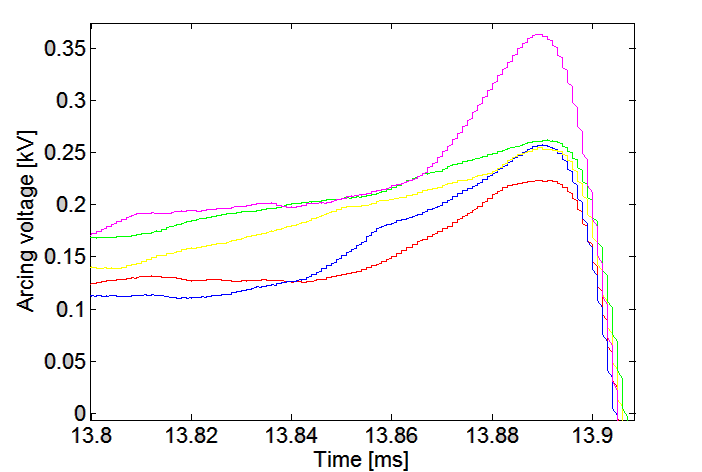
\includegraphics[scale=0.6, angle =0 ]{Bilder/Results/ArcingVoltage_18_none_reIgnition.PNG}
\caption{The arcing voltage for five interruption tests at 0.3 bar over-pressure and a current of 630 A. All the five tests where interrupted successfully at the second CZ, which occurred at approximately  x=18 mm.} \label{fig:18mmSuccessful}
\end{figure}

Based on the results presented in figure \ref{fig:18mmUnSuccessful} and \ref{fig:18mmSuccessful}, the average arcing voltage (blue line) for the the five unsuccessful interruptions and the five successful interruptions were calculated and presented in figure \ref{fig:18mmUnSuccessful_ave} and \ref{fig:18mmSuccessful_ave}. The two interruption tests from each of the two data collections which had the largest (green line) and smallest (red line) arcing voltage from the average arcing voltage are plotted together with it.


In figure \ref{fig:18mm_both_ave} the two average arcing voltages from figure \ref{fig:18mmUnSuccessful_ave} and \ref{fig:18mmSuccessful_ave} are plotted together. The green line is the average arcing voltage where the thermal re-ignitions occurred, while the magenta line is the average arcing voltage for the successful current interruptions.

\begin{figure}[H]
\centering
\includegraphics[scale=0.6, angle =0 ]{Bilder/Results/ArcingVoltage_18_reIgnition_average.PNG}
\caption{The average arcing voltage (blue line) for the five interruption tests at 0.3 bar over-pressure and a current of 630 A, together with the lowest (red line) and highest (blue line) arcing voltages obtained during testing. All the five tests experienced a thermal re-ignition at the first CZ, which occurred at approximately  x=18 mm.} \label{fig:18mmUnSuccessful_ave}
\end{figure}

\begin{figure}[H]
\centering
\includegraphics[scale=0.6, angle =0 ]{Bilder/Results/ArcingVoltage_18_none_reIgnition_average.PNG}
\caption{The average arcing voltage (blue line) for the five interruption tests at 0.3 bar over-pressure and a current of 630 A, together with the lowest (red line) and highest (blue line) arcing voltages obtained during testing. All the five tests where interrupted successfully at the first CZ, which occurred at approximately  x=18 mm.} \label{fig:18mmSuccessful_ave}
\end{figure}

\begin{figure}[H]
\centering
\includegraphics[scale=0.6, angle =0 ]{Bilder/Results/ArcingVoltage_18_both_average.PNG}
\caption{The average arcing voltage for both the successful (magenta line) and unsuccessful (green line) interruption tests.} \label{fig:18mm_both_ave}
\end{figure}

This arcing voltage experiment was conducted to see if a difference in arcing voltage could be observed between a successful and an unsuccessful current interruption. If such a measurable difference in the arcing voltages before CZ exists for the two interruption results, it might be possible to use this information to develop a simulation tool which can predict the outcome of the interruption based on this difference. In the paragraphs below, two possible theories to what may cause a difference in the arcing voltage between the two interruption outcomes are presented.

In cases where a successful interruption is obtained it is possible that the air flow cools the arc more efficiently than when a thermal re-ignition occur. A more efficient cooling of the arc may cause a temperature decrease in the plasma channel, where the current is flowing. As described by figure \ref{fig:condAir} in section \ref{sec:eleCondArc}, the conductivity of air is highly dependent on its temperature, therefore, it is possible that a more efficient cooling will result in a lower conductivity of the air. Since the current is unaffected by the arcing voltage and equal for all conducted tests, a decrease in conductivity will cause an increase in arcing voltage. Therefore, it is possible that a small difference in how the air flow cools the arc when the arc is successfully quenched, compared to when a thermal re-ignition occurs, causes an increase in the arcing voltage for a successful current interruption.

Another theory of how the arcing voltage will be different between the two interruption results is that it will be lower for a successful current interruption compared to an unsuccessful one. This is because a low arcing voltage will result in less dissipated energy. A smaller energy dissipation, especially close to CZ might result in a smaller amount of hot air and charge carriers that needs to be transported away to avoid a thermal re-ignition, which might be the difference between a successful and unsuccessful interruption of the current.

However, none of the two theories presented above could be confirmed with the two test series conducted in this arcing voltage experiment. If the average arcing voltage results from the tests conducted with the second CZ occurring at the position of x=75 mm are consulted, which are presented in figure \ref{fig:75mmUnSuccessful} and \ref{fig:75mmSuccessful}, it can be seen that the variance between each of the arcing voltages in the two figures is much larger than the difference between the two average arcing voltages presented in figure \ref{fig:75mm_both_ave}. This also applies to the test series with the first CZ occurring at x=18 mm, which are presented in figure \ref{fig:18mmUnSuccessful} and \ref{fig:18mmSuccessful}. If the picture sequence presented in appendix \ref{app:pictureSeq75mm} is consulted, no clear difference in the arc can be seen in the frames before CZ for the successful and unsuccessful current interruptions. If a difference in arcing voltage between a successful and an unsuccessful current interruption exists, more than five tests for each interruption case need to be conducted, since this might decrease the variance between them, and reveal a more distinct difference between the arcing voltages for the two interruption outcomes. However, the test set-up used to perform the arcing voltage tests in this report is not well suited for this task, since timing the CZ to occur at the right x-position, was challenging and many tests were discarded due to a wrong length of the arc at the moment of CZ.

Because no clear difference in the arcing voltage between a successful and unsuccessful current interruption could be confirmed by the two test series the arcing voltage might not be the best parameter to use in a simulation model which goal is to predict the interruption outcome. If the temperature in the arc could be measured directly, and not via the arcing voltage, it might be possible to find a difference in temperature which is related to the outcome of the interruption. This could be used to possibly link the temperature with how the air flow cools the arc. In section \ref{sec:HeatTransport} the heat distribution in an arc is presented, and as pointed out in this section the arc is cooled down by removing the stored heat in the "energy buffer zone" around the arc, not by cooling the arc directly with the air flow. When the amount of heat stored in this energy buffer zone is small, the temperature of the arc's core will decrease more rapidly than if a large amount of energy is stored there. Therefore, it is possible that the difference between a successful and an unsuccessful current interruption can be seen by a larger derivative of the temperature the last microseconds before CZ for a successful current interruption.


\newpage
%\subsection{Results and discussion based on picture sequences collected with the high-speed camera}
\subsection{Drop in arcing voltage} \label{sec:results_drop_arcing_voltage}

In figure \ref{fig:arcingVoltageDrop} the arcing voltage during an interruption test for geometry \textbf{b} at 880 A is presented. The arc experienced a thermal re-ignition at all three CZ crossings shown in the figure and a upstream over-pressure of 0.25 bar was used. The red square in figure \ref{fig:arcingVoltageDrop} shows a part of the graph where a steep drop in the arcing voltage occurred, this area is magnified in figure \ref{fig:arcingVoltageDrop_zoomed}. Both figures have been processed in matlab to filter out measuring noise. The filter used for noise cancelling was tuned so that it did not impact the steep drop in arcing voltage shown in the figure. It is not uncommon for steep drops in the arcing voltage to occur, and they often occur following a CZ. In appendix \ref{app:DROP_ImageSequences} another example of a voltage drop like the one presented here is shown. 

From figure \ref{fig:arcingVoltageDrop_zoomed}, it can be seen that the steep drop in arcing voltage occurred after approximately 1.3 ms after the third CZ. The voltage dropped from a peak of 425 V to 200 V using 60 $\mu$s, resulting in a voltage drop of 3.75 V$/  \mu$s. Frame 1 to 7 in the picture sequence from figure \ref{fig:arcingVoltage_drop_301_blue} shows the thermal re-ignition during the CZ, while frame 8 to 18 shows the arc for the time span upto and including the voltage drop. Frame 16 and 17 shows the arc during the steep drop in arcing voltage. 

From the picture sequence shown in figure \ref{fig:arcingVoltage_drop_301_blue}, it is quite clear what the causes the steep drop in arcing voltage. The arc do not burn in a straight line between the electrodes, but winds itself around. This winding is probably mostly caused by the hot air surrounding the arc, which rises and pulls the arc with it. After the CZ in frame 4, it can be seen that hot air near the pin contact have risen, and in frame 6 the arc re-ignites in this hot air channel, forming a curve. As the current increases and heating the arc further, the curve is elongated, while the distance between the start of the curve, and the pin contact decreases to the point where the curve short circuit between its starting point and the pin contact, causing the steep drop in arcing voltage shown in figure \ref{fig:arcingVoltageDrop_zoomed}. This winding and short circuit of the arc is also observed for the arcing voltage shown in appendix \ref{app:DROP_ImageSequences}.

 

\begin{figure}[H]
\centering
\includegraphics[scale=0.6, angle =0 ]{Bilder/Results/overviewArcingVoltageDrop.PNG}
\caption{Overview over the arcing voltage during an interruption tests spanning over three CZ. A steep drop in arcing voltage (marked by a red square) occurred after the third CZ.} \label{fig:arcingVoltageDrop}
\end{figure}

\begin{figure}[H]
\centering
\includegraphics[scale=0.6, angle =0 ]{Bilder/Results/zoomArcingVoltageDrop.PNG}
\caption{The area marked with the red square in figure \ref{fig:arcingVoltageDrop} magnified, showing the steep drop in arcing voltage.} \label{fig:arcingVoltageDrop_zoomed}
\end{figure}

\begin{figure}[H]
\centering
\includegraphics[scale=0.67, angle =0 ]{Bilder/Results/301_23_TR_TR_drop.png}
\caption{Picture sequence after a thermal re-ignition in the third CZ. The pictures shows the arc corresponding to the blue line in figure \ref{fig:arcingVoltageDrop_zoomed}, where a sudden voltage drop occurred approximately 1.5 ms after the CZ. The numbers in the corner of each picture indicates in what order the images where taken. The whole picture sequence spans over approximately 2 ms.} \label{fig:arcingVoltage_drop_301_blue}
\end{figure}

\newpage
\subsection{Current drop during dielectric re-ignition} \label{sec:dielectricReIgnitionResults}

For geometry \textbf{a} and \textbf{b} a few dielectric re-ignitions occurred, mostly when the pin was positioned inside of the cylindrical part of the nozzle. In figure \ref{fig:DR_disc_calc_areas} the voltage (black line) and current (blue line) during one of these dielectric re-ignitions are illustrated. The dielectric re-ignition shown in the figure occurred during a 880 A interruption test for geometry \textbf{b}, using an upstream over-pressure of 0.25 bar. The figure has been processed in matlab to filter out measuring noise.

Figure \ref{fig:DR_disc_calc_areas} has two squares marking two areas of the current. The red square marks an area where the current rises to a peak of about 160 A, and then falls to 40 A, during a time span of 70 $\mu$s. The decline of the current is best illustrated by an exponential decay which is described by equation \eqref{eq:expDecay}. The recovery voltage's peak reaches approximately 7.1 kV before the re-ignition occur. Some noise in the current measurement were not successfully removed from the figure, this is marked by the green square in figure \ref{fig:DR_disc_calc_areas}.

\begin{equation} \label{eq:expDecay}
I(t)=160e^{-0.0198t} \mathrm{A} \ \ \ \ \ \ \ \ \ \ t \in [0,70] \mu \mathrm{s}
\end{equation}

A picture sequence of the arc during the dielectric re-ignition displayed in figure \ref{fig:DR_disc_calc_areas} are shown in figure \ref{fig:DR_TR_305_1} and \ref{fig:DR_TR_305_2}. The picture sequence is split into two figures and some uninteresting frames are removed to shorten the sequence so that each of the figures fits a page. The numbers in each frame tells which order the frames follows within the picture sequence. In figure \ref{fig:DR_zoom_and_areas} the red square from figure \ref{fig:DR_disc_calc_areas} is magnified and vertical lines marking four time zones is included in the figure. Each time zone corresponds to different frames in the picture sequence presented below and the current in the arc the moment the picture where taken. Time zone "a" includes approximately frame one to six, where frame one illustrates that the arc have just re-ignited after the dielectric re-ignition and the current has started flowing. In time zone "b" the current is rising, which can be seen in the pictures as an increase in the intensity of the arc upto and including frame ten. Then the current has passed its peak at 160 A and decreases to approximately 40 A in frame 17, this time span represent time zone "c". In frame 18 the current starts to rise again, and it will quickly obtain its normal sinusoid shape, set by the supply side of the switch. In figure \ref{fig:DR_zoom_and_areas} this is represented by time zone "d".


\begin{figure}[H]
\centering
\includegraphics[scale=0.55]{Bilder/Results/DRplot_calc_areas.png}
\caption{Dielectric re-ignition during a 880 A interruption test for geometry \textbf{b}. The red square marks the area of interesst. The green square marks an area of the current suspected to be wrong due to measuring noise.} \label{fig:DR_disc_calc_areas}
\end{figure}

\begin{figure}[H]
\centering
\includegraphics[scale=0.55]{Bilder/Results/DRplot2_zoom.PNG}
\caption{The same dielectric re-ignition as shown in figure \ref{fig:DR_disc_calc_areas} but with the red area magnified. The vertical lines marks four time zones a, b, c, and d, which corresponds to different frames (a=[1,6], b=[7,10], c=[11,17], d=[18,22]) in the picture sequence from figure \ref{fig:DR_TR_305_1} and \ref{fig:DR_TR_305_2}.}
\label{fig:DR_zoom_and_areas}
\end{figure}

\begin{figure}[H]
\centering
\includegraphics[scale=0.7, angle =0 ]{Bilder/Results/305_75_DR_TR.png}
\caption{Picture sequence for the dielectric re-ignition shown in figure \ref{fig:DR_disc_calc_areas}. The numbers in the corner of each picture indicates in what order the images where taken.} \label{fig:DR_TR_305_1}
\end{figure}

\begin{figure}[H]
\centering
\includegraphics[scale=0.7, angle =0 ]{Bilder/Results/305_75_DR_TR_2.png}
\caption{Continuation of the picture sequence in figure \ref{fig:DR_TR_305_1} for the dielectric re-ignition shown in figure \ref{fig:DR_disc_calc_areas}. The numbers in the corner of each picture indicates in what order the images where taken.} \label{fig:DR_TR_305_2}
\end{figure}

%\begin{figure}[H]
%\centering
%\includegraphics[scale=0.40]{Bilder/Results/ATPdraw_lab_2.png}
%\caption{NA.} \label{fig:DR_ATP_OVER}
%\end{figure}

With the use of a circuit simulation tool called ATPdraw a current interruption in the test was simulated using the circuit from figure \ref{fig:testCurcuit} for a current of 880 A obtained with the circuit parameters from table \ref{tab:testParameters}. This simulation was conducted to find a possible cause for the current drop marked with the red square in figure \ref{fig:DR_disc_calc_areas}. The simulation performed in ATPdraw do not take the arcing voltage into consideration, and it is set to zero during the arcing time. This removes the effect of the arc from the system, and only the switching transient is analysed. Figure \ref{fig:DR_ATP_OVER} shows the simulation results for the voltage (black line) and current (blue line) during a dielectric re-ignition, with approximately the same time span between CZ and the re-ignition, as the one presented above. In figure \ref{fig:DR_ATP_ZOOM} the current during the re-ignition is magnified. As seen from the figure the same form of the current drop as seen in the measured results can be seen in the simulation results, however, the simulation results predict a considerable smaller current, which have a peak of about 45 A. With the use of ATPdraw it was possible to confirm that the drop in current is caused by the discharge of the capacitor (C), which occurs when the arc re-ignites. Simulations with different circuit parameters were conducted, but the magnitude of the measured drop in current was not possible to recreate, while still obtain the same recovery voltage and RMS value of the current.

The transaction between zero current and a high current, set by the voltage over the capacitor, which occurs when the arc re-ignites, happens over a very short time span ($<$1$\mu$s). Since the sampling rate of the hall effect current transducer used to measure the current is 100 kHz \cite{bib:HallEffect}, it is likely that the transaction occurs to fast to be accurately measured. This can also be seen in the picture sequence, since it seems unlikely that the measured current lowest value is 40 A, because in frame 17 in the picture sequence shows that the arc has almost extinguished at the lowest current magnitude after re-ignition.

Since the hall effect current transducer is not suited for a so fast change in current as experienced during a re-ignition, and the intensity of the arc shown in the picture sequence do not correspond well with the magnitude of the measured current, it is possible that the current is measured with a high error rate during the re-ignition of the arc. However, since both the measured and the simulated current shows a current drop it is likely that it is present, but that its magnitude is unknown. It is possible that a more accurate measurement of the current, especially close to CZ, can be obtained by the use of a Rogowski coil. A Rogowski coil is a kind of a transducer which is converting current to voltage. Through Faraday's law the induced voltage in the coil is proportional with the derivative of the current. The magnitude of the current can then be found via integration of its derivative, either with an integration circuit or with post processing of the measuring results. The integration circuit used, must be chosen so that it can handle the steep derivative of the current which occurs during a re-ignition of the arc. A Rogowski coil with an active integrator circuit can measure currents upto 5 MHz with sufficiently accuracy to measure switching impulse currents \cite{bib:SwitchingImpulseCurrent}, and might be applied in the test circuit for future current measurement during interruption testing, so that the current drop observed in figure \ref{fig:DR_disc_calc_areas} can be better analysed.

\begin{figure}[H]
\centering
\includegraphics[scale=0.65]{Bilder/Results/ATPdraw_Over_CurrentandVoltage_2_label.png}
\caption{Simulated recovery voltage and current during a dielectric re-ignition.} \label{fig:DR_ATP_OVER}
\end{figure}

\begin{figure}[H]
\centering
\includegraphics[scale=0.65]{Bilder/Results/ATPdraw_ZOOM_CurrentandVoltage_2_label.png}
\caption{Simulated recovery voltage and current during a dielectric re-ignition, when the current right after CZ is magnified.} \label{fig:DR_ATP_ZOOM}
\end{figure}
\newpage
%\subsection{Addressing uncertainties}
%\subsubsection{Data collection}

%\subsubsection{Voltage measurement} jeg tror jeg dropper dette kappittelet, skjønner ikke helt hva jeg skal få ut av det....


\cleardoublepage

\begin{comment}
\section{Discussion}
\subsection{The probability of interruption} 


\subsection{Arcing voltage considerations}

\subsection{Drop in arcing voltage} \label{sec:disc_drop_arcing_voltage}
Den deriverte er lik for begge eksemplene!

\subsection{Drop in current during dielectric re-ignition} \label{sec:disc_drop_current_DR}
\subsection{Durability of the arcing contacts} \label{fig:durability}


\newpage
\subsection{Suggestion for further work}
\subsubsection{A nozzle that minimises arc impact on air flow}


\subsubsection{Cone-shaped nozzle}

\cleardoublepage
\end{comment}


\section{Conclusion}
\subsection{Interruption tests}
noe

bla

\subsection{Arcing voltage between successful and unsuccessful interruptions}
Neither a visual or measurable difference in the arcing voltage can be seen.

\subsection{Drop in arcing voltage}
bla

bla
\subsection{Current drop during dielectric re-ignition}
bla

bla

\cleardoublepage

\begin{thebibliography}{10}
\bibitem{bib:SF6PI} L.G. Christophorou, J. K. Olthoff, and R.J. Van Brunt, "Sulfur hexafluoride and the electric power industry", \textit{IEEE Electrical Insulation Magazine, vol. 13, No. 5, pp. 20-24}, Oct. 1997.

\bibitem{bib:comSub} amesimpex.com, \url{http://www.amesimpex.com/images/unitised_sub_002.jpg}, 26.9.2013

\bibitem{bib:HVEbreak} M. Runde, "Current interruption in power grids", Trondheim: Norwegian University of Science and Technology, 2013

\bibitem{bib:GFALEAPI} E. Attar, P. Skryten, T. R. Bjortuft, P. Stoller, N. Ranjan, O. Granhaug, M. Schwinne and B. Wuethrich "Gas flow analysis in low energy arc puffer interrupters", \textit{22$^{nd}$ International Conference on Electricity Distribution CIRED, NO. 0410}, June 2013.

\bibitem{bib:CBAC} W. Rieder, "Circuit breakers, physical and engineering problems, III-Arc-medium considerations", \textit{IEEE spectrum, pp. 80-84}, Sept. 1970.

\bibitem{bib:IPSF6AQM} W. Hertz, H. Motschmann and H. Wittel, "Investigations of the properties of SF$_6$ as an arc quenching medium", \textit{Proceedings of The IEEE, vol. 59, NO. 4, pp. 485-492}, April 1971.

\bibitem{bib:TDCIGBB} W. Hermann, "Theoretical description of the current interruption in HV gas blast breakers", \textit{IEEE Transactions on Power Apparatus and System, vol. PAS-96, NO. 5, pp. 1546-1555}, Sept./ Oct. 1977.

\bibitem{bib:CIHVN} G. Frind and B. W. Swanson "Current Interruption in High-Voltage Networks", Baden: BBC Brown, Boveri \& Company Limited, 1977

\bibitem{bib:THFD} R. W. Johnson, "The handbook of fluid dynamics", Heidelberg: Springer-Verlag GmbH \& Co. KG, 1998.

\bibitem{bib:TET4160HVIM} E. Ildstad, "High voltage insulation materials", Trondheim: Norwegian University of Science and Technology, 2012, August 2012.

\bibitem{bib:KlimaKur2020} "KLIMAKUR2020", Oslo: Klima- og forurensningsdirektoratet, 2010

\bibitem{bib:consSF6} esrl.noaa.gov, \url{http://www.esrl.noaa.gov/gmd/webdata/iadv/ccgg/graphs/pdfs/ccgg.MLO.sf6.1.none.discrete.all.pdf}, 17.10.2013

\bibitem{bib:regSF6Miljo} regjeringen.no, \url{http://www.regjeringen.no/nb/dep/md/dok/regpubl/stmeld/2011-2012/meld-st-21-2011-2012/5/5.html?id=682932}, 21.10.2013

\bibitem{bib:StatSF6} K. L. Hansen, "Emissions from consumption of HFCs, PFCs and SF$_6$ in Norway", \textit{Statistics Norway/Department of Economic Statistics/Environmental Statistics}, 2007.

\bibitem{bib:AFIMVLBA} N. S. Aanensen, E. Jonsson, and M. Runde "Air flow investigation for a medium voltage load break switch", to be published.

\bibitem{bib:CIAMVLBS} E. Jonsson, N. S. Aanensen and M. Runde, "Current interruption in air for a medium voltage load break switch", \textit{IEEE Trans. Power Delivery}, in press.

\bibitem{bib:HallEffect} lem.com, \url{http://www.lem.com/docs/products/lt\%202000-s\%20sp42\%20e.pdf}, 14.5.2014

\bibitem{bib:SwitchingImpulseCurrent} W. Limcharoen and P. Yutthagowith, "Rogowski Coil with an Active Integrator for Measurement of Switching Impulse Current", \textit{10th International Conference on Electrical Engineering/Electronics, Computer, Telecommunications and Information Technology, pp. 1-4}, May 2013.

\end{thebibliography}

\cleardoublepage
\appendix
\vspace*{\fill}
\begingroup
\begin{center}
\huge Appendix
\end{center}
\endgroup
\vspace*{\fill}

\cleardoublepage

\section{Appendix: Picture sequece of the air blast} \label{app:SelfBlast}
\setcounter{figure}{0}
\makeatletter 
\renewcommand{\thefigure}{A.\@arabic\c@figure}
\makeatother

\setcounter{table}{0}
\makeatletter 
\renewcommand{\thetable}{A.\@arabic\c@table}
\makeatother
%tests
\begin{figure}[H]
\centering
\includegraphics[scale=0.475, angle =0 ]{Bilder/Results/selfBlast.jpg}
\caption{Picture sequence when the pin contact exits the cylindrical part of the nozzle, causing an air blast. The numbers in the corner of each picture indicates in what order the images where taken. In order to fit the sequence in one figure every second frame were removed from the sequence.} \label{fig:selfBlast_seq}
\end{figure}



\cleardoublepage

\section{Appendix: Picture sequences for arcing voltage tests} \label{app:pictureSeq75mm} %\label{app:ImageSequences}
\setcounter{figure}{0}
\setcounter{table}{0}
\makeatletter 
\renewcommand{\thefigure}{B.\@arabic\c@figure}
\makeatother

\makeatletter 
\renewcommand{\thetable}{B.\@arabic\c@table}
\makeatother

%\subsection*{The 75 mm arcing voltage test} 
\subsection{Thermal re-ignitions for the 75 mm arcing voltage test}
\begin{figure}[H]
\centering
\includegraphics[scale=0.7, angle =0 ]{Bilder/Results/073_75_TR_TR.png}
\caption{Picture sequence for a interruption attemt with a thermal re-ignition at the second CZ, which occurred at approximately x=75 mm. The pictures shows the arc corresponding to the red line in figure \ref{fig:75mmUnSuccessful}. The numbers in the corner of each picture indicates in what order the images where taken.} \label{fig:arcingVoltage_test_73_red_TR}
\end{figure}

\begin{figure}[H]
\centering
\includegraphics[scale=0.7, angle =0 ]{Bilder/Results/100_75_TR_TR.png}
\caption{Picture sequence for a interruption attemt with a thermal re-ignition at the second CZ, which occurred at approximately x=75 mm. The pictures shows the arc corresponding to the blue line in figure \ref{fig:75mmUnSuccessful}. The numbers in the corner of each picture indicates in what order the images where taken.} \label{fig:arcingVoltage_test_73_blue_TR}
\end{figure}

\begin{figure}[H]
\centering
\includegraphics[scale=0.7, angle =0 ]{Bilder/Results/116_75_TR_TR.png}
\caption{Picture sequence for a interruption attemt with a thermal re-ignition at the second CZ, which occurred at approximately x=75 mm. The pictures shows the arc corresponding to the yellow line in figure \ref{fig:75mmUnSuccessful}. The numbers in the corner of each picture indicates in what order the images where taken.} \label{fig:arcingVoltage_test_116_yellow_TR}
\end{figure}

\begin{figure}[H]
\centering
\includegraphics[scale=0.7, angle =0 ]{Bilder/Results/120_75_TR_TR.png}
\caption{Picture sequence for a interruption attemt with a thermal re-ignition at the second CZ, which occurred at approximately x=75 mm. The pictures shows the arc corresponding to the green line in figure \ref{fig:75mmUnSuccessful}. The numbers in the corner of each picture indicates in what order the images where taken.} \label{fig:arcingVoltage_test_116_green_TR}
\end{figure}

\begin{figure}[H]
\centering
\includegraphics[scale=0.7, angle =0 ]{Bilder/Results/143_75_TR_TR.png}
\caption{Picture sequence for a interruption attemt with a thermal re-ignition at the second CZ, which occurred at approximately x=75 mm. The pictures shows the arc corresponding to the magenta line in figure \ref{fig:75mmUnSuccessful}. The numbers in the corner of each picture indicates in what order the images where taken.} \label{fig:arcingVoltage_test_116_magenta_TR}
\end{figure}

\subsection{Successful interruptions for the 75 mm arcing voltage test}
\begin{figure}[H]
\centering
\includegraphics[scale=0.7, angle =0 ]{Bilder/Results/124_75_TR_OK.png}
\caption{Picture sequence for a successful interruption at the second CZ, which occurred at approximately x=75 mm. The pictures shows the arc corresponding to the red line in figure \ref{fig:75mmSuccessful}. The numbers in the corner of each picture indicates in what order the images where taken.} \label{fig:arcingVoltage_test_124_red_OK}
\end{figure}

\begin{figure}[H]
\centering
\includegraphics[scale=0.7, angle =0 ]{Bilder/Results/114_75_TR_OK.png}
\caption{Picture sequence for a successful interruption at the second CZ, which occurred at approximately x=75 mm. The pictures shows the arc corresponding to the blue line in figure \ref{fig:75mmSuccessful}. The numbers in the corner of each picture indicates in what order the images where taken.} \label{fig:arcingVoltage_test_114_blue_OK}
\end{figure}

\begin{figure}[H]
\centering
\includegraphics[scale=0.7, angle =0 ]{Bilder/Results/98_75_TR_OK.png}
\caption{Picture sequence for a successful interruption at the second CZ, which occurred at approximately x=75 mm. The pictures shows the arc corresponding to the yellow line in figure \ref{fig:75mmSuccessful}. The numbers in the corner of each picture indicates in what order the images where taken.} \label{fig:arcingVoltage_test_114_yellow_OK}
\end{figure}

\begin{figure}[H]
\centering
\includegraphics[scale=0.7, angle =0 ]{Bilder/Results/126_75_TR_OK.png}
\caption{Picture sequence for a successful interruption at the second CZ, which occurred at approximately x=75 mm. The pictures shows the arc corresponding to the green line in figure \ref{fig:75mmSuccessful}. The numbers in the corner of each picture indicates in what order the images where taken.} \label{fig:arcingVoltage_test_114_green_OK}
\end{figure}

\cleardoublepage

\section{Appendix: Drop in arcing voltage example} \label{app:DROP_ImageSequences}
\setcounter{figure}{0}
\setcounter{table}{0}
\makeatletter 
\renewcommand{\thefigure}{C.\@arabic\c@figure}
\makeatother

\makeatletter 
\renewcommand{\thetable}{C.\@arabic\c@table}
\makeatother

In figure \ref{fig:arcingVoltageDrop_2} the arcing voltage for a interruption test for geometry \textbf{c} at 630 A is presented. The arc had a thermal re-ignition in all three CZ shown in the figure when a upstream over-pressure of 0.3 bar was used. The red square in figure \ref{fig:arcingVoltageDrop_2} shows a part of the graph where a steep drop in the arcing voltage occurred. The area is magnified in figure \ref{fig:arcingVoltageDrop_zoomed_2}. Both figures have been processed in matlab to filter out measuring noise. The filter used for noise cancelling was tuned so that it did not impact the steep drop in arcing voltage shown in the figures.

From figure \ref{fig:arcingVoltageDrop_zoomed_2}, it can be obtained that the steep drop in arcing voltage occurred after approximately 1.0 ms after the third CZ. The voltage dropped from a peak of 480 V to 320 V using 50 $\mu$s, resulting in a voltage drop of 3.2 V$/  \mu$s. Picture 1 to 4 in figure \ref{fig:arcingVoltage_drop_301_blue_2} shows the thermal re-ignition during the CZ, while picture 5 to 16 shows the arc for the time span upto and including the voltage drop. Picture 14 and 15 shows the arc during the steep drop in arcing voltage.

\begin{figure}[H]
\centering
\includegraphics[scale=0.6, angle =0 ]{Bilder/Results/overviewArcingVoltageDrop_2.PNG}
\caption{Overview over the arcing voltage during an interruption tests spanning over three CZ. A sudden drop in arcing voltage (marked by a red square) occurred after the third CZ.} \label{fig:arcingVoltageDrop_2}
\end{figure}

\begin{figure}[H]
\centering
\includegraphics[scale=0.6, angle =0 ]{Bilder/Results/zoomArcingVoltageDrop_2.PNG}
\caption{The area marked with the red square in figure \ref{fig:arcingVoltageDrop} magnified, showing the sudden drop in voltage.} \label{fig:arcingVoltageDrop_zoomed_2}
\end{figure}

\begin{figure}[H]
\centering
\includegraphics[scale=0.67, angle =0 ]{Bilder/Results/301_23_TR_TR_drop_2.png}
\caption{Picture sequence after a thermal re-ignition in the third CZ. The pictures shows the arc corresponding to the blue line in figure \ref{fig:arcingVoltageDrop_zoomed}, where a sudden voltage drop occured approximatly 1.0 ms after the CZ. The numbers in the corner of each picture indicates in what order the images where taken.} \label{fig:arcingVoltage_drop_301_blue_2}
\end{figure}

%\section{Appendix: Matlab code for sortVoltage.m} %husk å oppdatere denne!!
%\lstinputlisting[language=Matlab]{sortVoltage.m}

\end{document}
